\documentclass[12pt]{article}
\usepackage{fullpage}
\usepackage{amssymb}
\usepackage{graphics} 
\usepackage{amsmath}
\usepackage[color=yellow]{todonotes}
\usepackage{url}
\usepackage{xcolor}
\usepackage{longtable}
\usepackage[hidelinks]{hyperref}
\usepackage{bbm}

\usepackage{natbib}

\newenvironment {proof}{{\noindent\bf Proof }}{\hfill $\Box$ \medskip}

\newtheorem{theorem}{Theorem}[section]
\newtheorem{lemma}[theorem]{Lemma}
\newtheorem{condition}[theorem]{Condition}
\newtheorem{proposition}[theorem]{Proposition}
\newtheorem{remark}[theorem]{Remark}
\newtheorem{hypothesis}[theorem]{Hypothesis}
\newtheorem{corollary}[theorem]{Corollary}
\newtheorem{example}[theorem]{Example}
\newtheorem{definition}[theorem]{Definition}
\newtheorem{notation}[theorem]{Notation}

\renewcommand{\theequation}{\arabic{section}.\arabic{equation}}
\def \non{{\nonumber}}
\def \hat{\widehat}
\def \tilde{\widetilde}
\def \bar{\overline}
\newcommand{\IP}{\mathbb P}
\newcommand{\IQ}{\mathbb Q}
\newcommand{\IE}{\mathbb E}
\newcommand{\IR}{\mathbb R}
\newcommand{\IZ}{\mathbb Z}
\newcommand{\IN}{\mathbb N}
\newcommand{\IT}{\mathbb T}
\newcommand{\IC}{\mathbb C}
\newcommand{\ind}{\mathbf{1}}
\newcommand{\bigO}{\mathcal{O}}
\newcommand{\grad}{\nabla}
\newcommand{\dif}{\mathrm{d}\,}

%%%%%%% notation
\newcommand{\DG}{\mathcal{B}}  % generator of the dispersal process
\newcommand{\DD}{\mathcal{D}}  % the second-order part of the generator of dispersal
\newcommand{\meanq}{\vec b}    % mean of dispersal, times theta
\newcommand{\covq}{C}     % covariance matrix of dispersal, times theta
\newcommand{\kernel}{\rho}  % interaction kernels
\newcommand{\smooth}[1]{\kernel_{#1} \! * \!}  % convolution by the interaction kernel
\newcommand{\wavespeed}{\mathfrak{c}}    % speed (vector) of a wave
\newcommand{\Lgen}{\mathcal{L}}    % generator of a lineage
\newcommand{\Pgen}{\mathcal{P}}    % generator of the population process
\newcommand{\lp}{\xi}              % process with levels
\newcommand{\labelspace}{\mathcal{I}} % space of labels
\newcommand{\concat}{\oplus}   % concatenation of labels
\newcommand{\measures}{\mathcal{M}_F(\IR^d)} % finite measures on Rd


\newcommand{\plr}[1]{\todo[inline]{Peter: #1}}
\newcommand{\comment}[1]{{\color{blue} \it #1}}

\begin{document}

\title{\large{\bf
Looking forwards and backwards through locally regulated populations
}}

% OTHER IDEAS:
% A class of nonlinear superprocesses
% Uncovering genealogical structures of locally regulated populations with lookdown constructions on nonlinear superprocesses
                                                       
\author{ \begin{small}
\begin{tabular}{ll}                              
Alison M. Etheridge 
 & Thomas G. Kurtz \\   
Department of Statistics & Departments of Mathematics and Statistics\\       
Oxford University & University of Wisconsin - Madison \\                   
24-29 St Giles & 480 Lincoln Drive\\                                                         
Oxford OX1 3LB & Madison, WI  53706-1388\\
UK & USA \\                        
etheridg@stats.ox.ac.uk & kurtz@math.wisc.edu     \\
\url{http://www.stats.ox.ac.uk/~etheridg/} & 
\url{http://www.math.wisc.edu/~kurtz/}  \\       \\
\\
Ian Letter&  Peter L. Ralph 
\\   
Department of Statistics & Department of Mathematics \\
Oxford University &University of Oregon\\                   
24-29 St Giles & Fenton Hall\\
Oxford OX1 3LB & Eugene, OR 97403-1222\\
UK & USA \\
restucci@stats.ox.ac.uk  & plr@oregon.edu \\
\url{https://www.stats.ox.ac.uk/~restucci/}&
\url{https://math.uoregon.edu/profile/plr} \\
\\
Terence Tsui 
 &  \\   
Department of Statistics & \\
Oxford University & \\                   
24-29 St Giles& \\
Oxford OX1 3LB & \\
UK & \\
terence.tsui@sjc.ox.ac.uk &      \\
\url{https://www.maths.ox.ac.uk/people/terence.tsui}&  \\
\end{tabular}
\end{small}}

\date{\today}
\maketitle


\begin{abstract}

We do something...

\vspace{.1in}


\noindent {\bf Key words:}  population model, nonlinear superprocess, 
lookdown construction, porous medium equation, 
reaction-diffusion equation, travelling waves, genealogies,


\vspace{.1in}



\noindent {\bf MSC 20}10 {\bf Subject Classification:}  Primary:  
%60J25, 92D10, 92D15, 92D25 92D40  
\\Secondary:   %60F05, 60G09, 60G55, 60G57, 60H15, 60J68
 
\end{abstract}
\tableofcontents
\newpage

\comment{TODO: talk about $N \to \infty$ rather than $\theta \to \infty$.}

%%%%%%%%%%%%%%%%%%%%%%%
\section{Introduction}

\comment{I think the introduction covers a good set of things in a good order, it's just a bit long.}

As one takes a journey, long or short, the landscape changes:
forests thicken or thin or change their composition,
springtime grasslands host intergrading mosaics of different types of flowers.
The aim of this paper is to understand the implications of a broad class of mechanistic spatial models
that might describe how such populations live, die, and reproduce:
How does population density change across space and time?
And, how might we learn about the underlying dynamics from genealogical or genetic data?
We work with individual-based models of a single species in continuous space,
where birth, death and establishment may all depend on spatial location
as well as on local population density, allowing for stable populations through density-dependent feedback.

There is now a huge literature devoted to spatial branching processes,
including branching random walk, 
branching Brownian motion, and the Dawson-Watanabe superprocesses.  
In addition to possessing a rich and beautiful mathematical structure, 
the superprocesses are remarkable for demonstrating a certain `universality', 
arising, as they do, as scaling limits of a vast array of different 
spatial population models \cite[e.g.,][]{chetwynd-diggle/etheridge:2018,
cox/perkins:2005,
cox/durrett/perkins:1999,
cox/durrett/perkins:2000,
holmes:2008,
vanderhofstad/sakai:2010,
vanderhofstad/slade:2003,
vanderhofstad/holmes/perkins:2017}.

These models make mathematical sense in very general spaces, but
in biological applications, typically, 
individuals are assumed to be scattered across one or two-dimensional
Euclidean space. In that setting, it is well known that, 
in the long term, the population will either 
die out, or it will develop clumps of arbitrary density and extent. 
To counter this, it is common to
impose some local regulation by either increasing death rates, or 
reducing birth rates, in proportion to the local population density,
so that the population has a tendency to grow in sparsely populated regions
and shrink where it is overcrowded. This leads to spatial analogues of  
logistic branching processes.

Although it can be more mathematically convenient to work with branching
Brownian motions, in many settings it is biologically more natural to 
develop models based on branching random walk.  
Individuals produce a random number of offspring,
that are thrown off according to some (usually symmetric) 
distribution centred on the location of the parent.   
This is particularly appropriate for modelling plant populations, in which
this dispersal of offspring around the parent is the only source of
spatial motion.


Most models do not distinguish between juveniles and adults, so,
for example, the number of adults produced by a single parent is determined
by the degree of crowding at the location of the parent. The novelty
of the models that we introduce here is that, although we shall only
follow the adult population, in formulating the dynamics of the
models we shall distinguish
between production of juveniles, which will depend upon the location of 
the adult, and their successful establishment, which will depend on the
location in which a juvenile lands. The result is that not only the absolute 
number, but also the spatial distribution
around their parent, 
of those offspring that survive to adulthood
will depend upon the local population 
density. 


We shall consider different classes of scaling limits for our model; the first class consisting of
(generalised) super-processes limits, and the second class where the limits are deterministic. In the
superprocess setting, for our approach to work we measure the local population
density at a point by integrating against a smooth test function, for example 
a Gaussian density centred on that point.  
When the limit is deterministic,
we can simultaneously reduce the parameter in that Gaussian density so that,
in the limit, the local population density is simply the population density 
at that point. Nonetheless, we retain a signal of our two stage approach
to modelling reproduction, and  
in this way we recover a nonlinear partial differential equation. 
This approach requires some technical conditions that we will verify in two important examples,
the porous medium equation with a logistic growth term of the form 
$$\partial_t \varphi = \Delta (\varphi^2)+\varphi(1-\varphi),$$
and a wide class of semi-linear partial differential equations of the form 
$$\partial_t \varphi = \Delta\varphi+ \varphi \left(G(\varphi)-H(\varphi)\right),$$
which include the Fisher-KPP equation and the Allen-Cahn equation.

The porous medium equation (PME)
is a degenerate nonlinear diffusion equation that
has been the subject of intensive study. We refer to~\cite{vazquez:2007} for 
a comprehensive reference. The equation has also been studied with various
forms of noise, see~\cite{barbu/daprato/roeckner:2016}, although not the 
form of noise that will arise from the population dynamics below. 
Deriving nonlinear diffusion equations as limits of weakly interacting 
diffusions goes back at least to~\cite{mckean:1967}, and this 
programme has been
carried out for the PME and its generalisations. 
The degeneracy of the PME
results in some extra analytic
challenges,~\cite{jourdain:2000}.
Recent work in this 
direction has been spurred on by applications
in mathematical finance, %where the porous medium arises 
in particular, in the study of weak limits of systems
of diffusions interacting through their 
rank,~\cite{dembo/shkolnikov/varadhan/zeitouni:2016, jourdain/reygner:2013}
and references therein.
Our approach is different.
We start from individual
based population models, thus providing a microscopic mechanism that leads to 
nonlinear diffusion.
Other microscopic mechanisms have been proposed in the special case of the
PME, see 
e.g.~\cite{feng/iscoe/seppalainen:1997, oelschlaeger:1990}; ours
is specifically motivated by biological considerations.




Another novelty of our models stems from the use of lookdown construction to retain the dynamics of lines of descent in our population while passing to a scaling limit. The lookdown construction is first introduced in \cite{donnelly/kurtz:1996} to provide a mechanism to trace lineages while passing through a scaling limit for the Moran model. In more recent works, see~\cite{kurtz/rodrigues:2011, etheridge/kurtz:2018}, lookdown constructions are further applied into models of branching populations with spatial structures. In \S \ref{Sec: Lookdown Constructions}, we follow closely the techniques presented in these papers to impose lookdown constructions for our models which allow us to retain information about ancestry of individuals in the population as we pass to a large population limit. This in turn allows us to write down an explicit expression for the generator of the position of ancestral lineages with respect to the travelling wave fronts for populations modelled by a huge class of semi-linear partial differential equations, see Theorem \ref{teo:ancestral lineages}.
This attempt is novel and we have provided the first ever rigorous proof to similar results on ancestral lineages. This result allows us to compare ancestral lineages of individuals sampled from the front of a population evolving according to the PME with logistic growth to those under the Fisher-KPP and Allen-Cahn equations. For example, as a result of the nonlinear diffusion, 
for suitable initial conditions, the solution to the one-dimensional 
porous medium equation with logistic growth converges to a travelling
wave with a sharp cut-off; i.e., in contrast to the classical 
Fisher KPP equation, the solution at time $t$
vanishes beyond $x=x_0+ct$ for some constant wavespeed
$c>0$, \cite{kamin/rosenau:2004}.

\comment{Need a transition or otherwise to merge this with the above.}
The history of a natural population is often only accessible indirectly 
through patterns of genetic diversity that have been laid down. From 
genetic data, one can try to infer the genealogical trees that relate 
individuals in a sample from the population. It is therefore of interest
to establish the distribution of genealogical trees relating individuals
sampled from a population evolving according to any proposed mathematical
model.

In general this is an extremely difficult question. However, in special
circumstances, some progress can be made. One of the settings that
has received a great deal of attention in recent years is that in which 
a population is expanding into new territory as a travelling wave. 
Typically one considers a stationary wavefront moving across $\IR^1$, and
most work has focussed on the classical Fisher-KPP equation with a 
stochastic term, i.e.
$$dw=\big(\Delta w +sw(1-w)\Big)dt +\sqrt{\frac{\alpha(w)}{N}}W(dt,dx),$$
where $W$ is space-time white noise, and $N$ is a measure of the 
local population density. The coefficient
$\alpha(w)$ is generally taken to be either
$w$, corresponding to a superprocess limit, or $w(1-w)$ giving a 
spatial analogue of a Wright-Fisher diffusion. The first is 
appropriate for modelling the range of an expanding population,
the second for the spread of a selectively advantageous 
mutation through an established (selectively neutral) population. 
Because of the logistic control of the growth rate,
individuals in the wavefront can have much greater reproductive success
than those in the `bulk' of the expanding population. 
Tracing backwards in time, individuals sampled
from behind the wave are `caught' by the wave, upon which they become
trapped in the wavefront. If the population density is very high, then over
suitable timescales, the genealogical trees will be dominated by 
periods of extremely rapid coalescence corresponding to a significant 
proportion of the individuals in the front being descended from a particularly
reproductively successful ancestor. For a surprisingly wide range of models, 
it is believed that, for very large $N$ and on suitable timescales, 
genealogies converge to a 
Bolthausen-Sznitman coalescent, e.g.~\cite{brunet/derrida/mueller/munier:2007}. 
On the other hand, if one replaces the logistic growth term of the classical
Fisher-KPP equation with a nonlinearity that reflects cooperative
behaviour in the population, such as
$$wF(w)=w(1-w)(Cw-1),$$
then, for sufficiently large $C$ (strong cooperation),
the nature of the deterministic
wave changes from `pulled' to `pushed', \cite{birzu/hallatschek/korolev:2017}.
In that setting, the genealogies will also be quite different
from the Fisher-KPP case. For example, \cite{etheridge/penington:2020}
shows that for a discrete space model corresponding to this 
nonlinearity with $C>4$, after suitable scaling, the genealogy of a
sample converges not to a Bolthausen-Sznitman coalescent, but to
a Kingman coalescent. 
\todo[inline]{Is that condition $C>4$ correct? the paper with Sarah is done for the equation $\partial_t u = \Delta u + u(1-u)(2u-1+\alpha)$ and valid for $\alpha \in (0,1)$. Factorising we would get that equation would be $\partial_t u = \Delta u + (1-\alpha) u(1-u)(\frac{2}{1-\alpha}u-1)$. Supposing the $(1-\alpha)$ in front does not affect the result (which I suppose wouldn't) we get that $C= \frac{2}{1-\alpha}$ and so $\alpha \in (0,1)$ if and only if $C>2$ ...}
The reason, roughly, is that ancestral lineages
settle to a stationary distribution relative to the position of the 
wavefront which puts very little weight close to the `tip' of the wave, so
that when ancestral lineages meet,
it is typically in a location where population density is
high, where no single ancestor produces a disproportionately large number of 
descendants in a short space of time. 

As a first step towards understanding what we should expect in models with
nonlinear diffusion, we consider the position of an ancestral lineage
relative to the wavefront in the deterministic models, and compare that 
to what we see for a classical Fisher-KPP equation. 
In~\S\ref{sec: wright-malecot}, we then indicate how to extend these ideas to 
extract information about relatedness between two individuals in the 
superprocess limit, at least when population intensity is very high, and
we present some evidence to support the conjecture that genealogies 
for populations expanding according to 
our superprocess models with nonlinear diffusion
can be very different from those under 
the classical Fisher-KPP equation. 

% % % % % % % % % % % % % %
\subsection{Structure of the paper}

In the paper we study scaling limits of spatial populations,
obtaining convergence of both the population process
(i.e., the population density as a function of time,
although strictly speaking it is a measure that may not have a density)
as well as of lineages traced back through such a population.
We retain linages through the rescaling process
by means of a lookdown construction.
First, in section~\ref{sec: Model and main results},
we describe the model and the main theorems
(Theorems~\ref{thm:nonlocal_convergence}, \ref{thm:local_convergence}, and~\ref{thm:lineages}).
Next, in Section~\ref{sec:applications}, we discuss a few striking consequences of these results,
namely, X Y and Z \comment{TODO}.
In section \ref{sec:heuristics}, we provide heuristic explanations
of why the theorems ought to be true,
and some key ideas behind them.
In Section \ref{sec:lookdown} we define and discuss the lookdown process that retains the levels.
This is followed by the technical proofs in section \ref{sec:proofs}.



%%%%%%%%%%%%%%%%%%%%%%%%%%%%%%%%
\section*{Notes to ourselves}

\plr{For recording/discussing notation decisions.}

$X$ is the original, unscaled process,
and $\eta(t) = X(t\theta)/N$.

When the process has a density, it is $\varphi(t, x) = d \eta_t(dx)/dx$.

$$\lim \frac{\theta}{N} =: \alpha$$

Were not using $\lambda$, but only $N$.

%%%%%%%%%%%%%%%%%%%%%%%%%%%%%%%%
\section{Model and main results}
    \label{sec: Model and main results}

The model we work with is a fairly general model
of individuals living in continuous space.
We start with a population of
$\bigO(N)$ individuals per unit area distributed in $\mathbb{R}^d$.
For applications, $d=1$ or $d=2$, but our results apply more generally.
The population will be distributed over a bounded region,
so the total number of individuals will also be $\bigO(N)$.
The population changes in continuous time, and
we describe the state of the population at time $t$ with a counting measure $X(t)$,
which assigns one unit of mass to the location of each individual.

Population dynamics are controlled by three quantities,
birth ($\gamma$), establishment ($r$), and death ($\mu$),
each of which can depend on spatial location and local population density
in a way we specify later.
Each individual gives birth at rate $\gamma$ to a single offspring,
and the offspring
then disperses according to a kernel $q(\cdot)$ away from the location of the parent.
We assume that $q$ is the density of a multivariate Gaussian,
allowing a nonzero mean and anisotropic variance.
Both the mean and covariance can change across space,
but do not depend on population density.
The offspring does not necessarily survive to be counted in the population:
it ``establishes'' with probability $r$,
or else it dies immediately.
Independently, each individual dies with rate $\mu$.

We aim to obtain universal behavior by taking the density, $N$, to infinity,
and also scaling time by a factor of $\theta$,
so that defining $\eta(t) = X(\theta t) / N$,
the process $\{\eta(t)\}_{t \ge 0}$
will converge to a suitable measure-valued process
as $N$ and $\theta$ tend to infinity,
with the nature of the limit depending on how they tend to infinity together.
Demographic rates in our model
will be determined by local population density relative to $N$,
so that population dynamics depend more naturally on $\eta$ (rather than $X$).
However, to avoid confusion arising from the time scaling,
we describe the model in terms of $X$ next.
See Figure~\ref{fig:model_setup} for a conceptual depiction.

\begin{figure}
    \begin{center}
        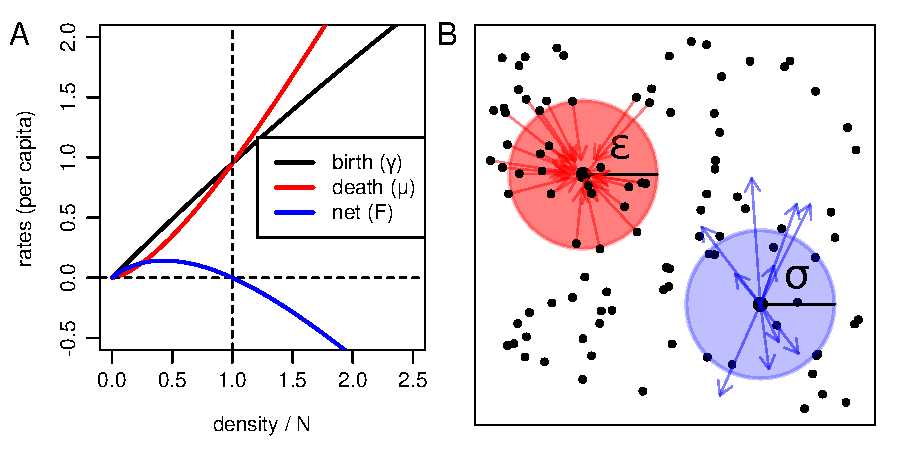
\includegraphics{figures/conceptual_figure}
    \end{center}
    \caption{
        \comment{Perhaps we should have two panels, one with the PME example (currently panel A) and the other with FKPP;
        right now panel B is not very helpful I think, so maybe should be omitted or added to so it better describes the whole process
        (including dispersal and establishment).}
        Conceptual figure of the model.
        \textbf{(A)} Example plot of $\gamma$, $\mu$, and $F$
        (calculated here with $r=1$) against scaled local population density.
        In this example, both birth and death rates increase with population density,
        but death increases faster,
        and equilibrium occurs where they cross
        (and hence where $F=0$).
        \textbf{(B)} Cartoon of interaction ($\epsilon$) and dispersal ($\sigma$) distances.
        \label{fig:model_setup}
    }
\end{figure}

Birth, establishment, and death can depend on the location of the individual
and the local population density.
Since we would like the population density to scale with $N$,
these are functions of $X/N$, i.e.,
the counting measure with mass $1/N$ placed at the location of each individual.
To measure local population density, we convolve the population measure with
an ``interaction kernel'' -- which, for simplicity, we take to be Gaussian,
which we write as
$$
    p_{\epsilon^2}(x) := \frac{1}{(2 \pi \epsilon^2)^{d/2}} e^{-\|x\|^2 / 2 \epsilon^2} ,
$$
for an ``interaction distance'' $\epsilon$.
First consider birth rates, defined by
a nonnegative function $\gamma(x, m) : \IR^d \times \IR_{\ge 0} \to \IR_{\ge 0}$
of location $x$ and local population density $m$,
and an interaction distance $\epsilon_\gamma > 0$.
Local population density enters through the convolution of $X$ with $p_{\epsilon_\gamma^2}$,
which we write as $\smooth{\gamma} X$.
Then, the birth rate of an individual at location $x$ when the state of the population is $X$
is $\gamma(x, \smooth{\gamma} X(x) / N)$.
Similarly, the establishment probability of an offspring at location $x$ is
is $r(x, \smooth{r} X(x) / N)$,
where $r(x, m) : \IR^d \times \IR_{\ge 0} \to [0, 1]$
and again $\smooth{r} X$ is the convolution of $p_{\epsilon_r^2}$ with $X$.
Rather than defining a function $\mu(x, m)$ for the death rate,
it turns out to be more convenient to parameterize in terms of the net reproductive rate,
which we denote by $F(x, m)$,
scaled by $1/\theta$
so that the population density changes over a time scale of $\theta$.
(This corresponds to a ``near-critical branching'' assumption.)
Informally, we would like that
$$
    F = \theta (r \gamma - \mu) ,
$$
and to arrange this we define
the death rate of an individual at $x$ to be
\begin{align} \label{eqn:mu_defn}
    \mu
    =
    \max\left\{0, 
        r(x, \smooth{r} X(x) / N) \gamma(x, \smooth{\gamma} X(x) / N)
        - \frac{1}{\theta} F(x, \smooth{F} X(x) / N)
    \right\} ,
\end{align}
where again $F(x, m) : \IR^d \times \IR_{\ge 0} \to \IR_{\ge 0}$
and $\kernel_F = p_{\epsilon_F^2}$.

In summary, each of the three demographic parameters depend on local density measured
with a Gaussian kernel with possibly different scales:
for birth over a scale of $\epsilon_\gamma$,
for establishment over a scale of $\epsilon_r$,
and for net reproductive rate over a scale of $\epsilon_F$.
Note that death rates depend in principle on population densities at three different scales,
so that we could write $\mu = \mu(x, \smooth{\gamma} X(x) / N, \smooth{r} X(x) / N, \smooth{F} X(x) / N)$.
It might seem like
we have introduced unnecessary complexity
with these three different spatial scales on which interactions occur.
However,
it will turn out to be useful in the proofs to have $\epsilon_r < \epsilon_\gamma$,
although in the limit they can be taken equal to each other
(and $\epsilon_F$ is unconstrained),
so informally we think of local density as being determined on a scale of $\epsilon$.

\begin{remark}
Although this model allows fairly general birth and death mechanisms,
there are a number of limitations.
Perhaps most obviously, to simplify the notation
individuals give birth to only one offspring at a time,
although this restriction could be easily lifted
\citep[as in][]{etheridge/kurtz:2018}.
Furthermore, individuals do not move during their lifetime,
and the age of an individual does not affect their fecundity or death rates.
Finally, there is no notion of mating,
so availability of mates will not restrict the spread of a population,
and the lineages we follow will be uniparental.
For these reasons, the model is most obviously applicable to bacterial populations or selfing plants,
although we do not anticipate that incorporation of these complications
will change the general picture.
\end{remark}

We next summarize the dynamics of the rescaled model $\eta(t) = X(\theta t)/N$,
and state some assumptions on the parameters.
The process takes values in the space of finite measures on $\IR^d$,
which we write as $\measures$.

\begin{definition}[Model parameterization and assumptions]
\label{def:model_setup}
Suppose $\gamma(x, m)$, $r(x, m)$, and $F(x, m)$
are bounded, uniformly continuous functions
from $\IR^d \times \IR_{\ge 0}$ to $\IR_{\ge 0}$.
Furthermore, suppose $r$ takes values in $[0, 1]$
and has uniformly bounded second derivatives,
and that $(x, m) \mapsto m^2 \gamma(x, m)$ is uniformly bounded.
Fix nonnegative values $\epsilon_r$, $\epsilon_\gamma$, and $\epsilon_F$,
with $\epsilon_r < \epsilon_\gamma$.
Suppose $F: \IR^d \times \IR_{\ge 0} \to \IR$ is bounded and uniformly continuous
and define
\begin{align} \label{eqn:mu_defn}
    \mu(x, \eta)
    =
    r(x, \smooth{r} \eta(x))
    \gamma(\smooth{\gamma} \eta(x))
    - \frac{1}{\theta}
    F(x, \smooth{F} \eta(x)) .
\end{align}
\end{definition}

Expressions like $\gamma(x, \smooth{\gamma} \eta(x))$ will appear often in the paper.
To make formula more readable, we overload notation to define
$$
    \gamma(x, \eta) := \gamma(x, \smooth{\gamma} \eta(x)) ,
$$
and similarly write $\mu(x, \eta)$  for $\mu(x, \smooth{\mu} \eta(x))$ and $r(x, \eta)$ for $r(x, \smooth{r} \eta(x))$.
When convenient, we may also suppress the arguments completely,
writing simply $\gamma$, $\mu$, and $r$ for these quantities.

For each $N > 0$ and $\theta \ge 1/(\epsilon_\gamma - \epsilon_r)$,
the process $\left(\eta^N(t)\right)_{t \ge 0}$
is the continuous-time measure-valued Markov process described above
with birth rates, establishment probabilities, and death rates
determined as follows.
When the state of the process is $\eta \in \measures$,
offspring of mass $1/N$ are produced at location $x$
with rate $\theta \gamma(x, \eta) N \eta_s(dx)$
and adults die at location $x$ with rate $\theta \mu(x, \eta) N \eta_s(dx)$,
(i.e., at rates $\theta \gamma$ and $\theta \mu$ per capita respectively).
Each offspring disperses to a location offset from the parent's location
by an independent Gaussian with mean $\meanq(x) / \theta$
and covariance matrix $\covq(x) / \theta$;
an offspring at $x$ establishes instantaneously
with probability $r(x, \eta)$, or else dies.

We have just effectively defined the process, but to be completely clear,
we will now give a formal definition as a solution to a martingale problem.

\begin{definition}[Martingale Problem Characterisation]
    \label{defn:mgale_construction},
We define $(\eta^N_t)_{t \geq 0}$ to be the solution to the Martingale Problem,
with initial condition $\eta^N_0 \in \measures$,
such that for all smooth functions $f \in C^{2}_{0}(\mathbb{R}^d)$,
writing $\langle f, \eta \rangle = \int_{\IR^d} f(x) \eta(dx)$
and $q_\theta(x, dy)$ as the Gaussian kernel
with mean $x + \meanq(x)/\theta$ and covariance $\covq(x) / \theta$,
\begin{equation}
    \label{eq: Pre-limit Martingale Characterisation}
\begin{aligned}
M^N_t(f)
&:=  \langle f, \eta^N_t \rangle
        -\langle f, \eta^N_0 \rangle
 \\ &\qquad {}
 -  \int_{0}^{t}\bigg\{
        \int\left( \int \theta
             \left(
                f(z)r(z, \eta^N_{s})
                - f(x)r(x, \eta^N_{s})
            \right)
        q_\theta(x,dz) \right)
\\ & \qquad \qquad \qquad \qquad {}
        \times \gamma(x, \eta^N_{s}) \eta^N_{s}(dx)
\\ & \qquad \qquad {}
    + \int f(x) F(x, \eta^N_{s}) \eta^N_{s}(dx)
    \bigg\} ds
\end{aligned}    
\end{equation}
is a martingale with quadratic variation
\begin{equation}
\begin{aligned} \relax
[ M^N_t(f)] =& 
\frac{\theta}{N} \int_{0}^{t}\bigg\{
    \langle \gamma(x, \eta^N_{s})
        \int f^2(y)r(y, \eta^N_{s}) q_\theta(x,dy) 
    , \eta^N_{s}(dx) \rangle \\
& \qquad \qquad {}
    + \langle \mu(x, \eta^N_{s}) f^2(x) 
    , \eta^N_{s}(dx)\rangle
    \bigg\}ds. 
\end{aligned}    
\end{equation}
\end{definition}

Note that
since individuals are produced at rate $N \gamma \eta$ but have mass $1/N$ each,
these factors of $N$ cancel in~\eqref{eq: Pre-limit Martingale Characterisation}.
Since we are taking a diffusion limit,
we will have use for the following notation:

\begin{definition}[Dispersal generator]
    \label{def:dispersal_generator}
    Recall that we have defined the dispersal kernel,
    $q_\theta(x, dy)$,
    to be the density of a multivariate Normal
    with mean $\meanq(x)/\theta$ and covariance matrix $\covq(x)/\theta$
    (although sometimes we omit the dependence of $\meanq$ and $\covq$ on $x$).
    This implies that if we define, for $f : \IR^d \to \IR$,
    \begin{align}
    \DG f(x)
        =
        \sum_{ij} \covq(x)_{ij} \partial_{x_i} \partial_{x_j} f(x)
        + \sum_i \meanq(x)_i \partial_{x_i} f(x)
    \end{align}
    then
    \begin{align}
        \theta \int \left(
            f(y) - f(x)
        \right) q_\theta(x, dy)
    \to \DG f(x) 
        \qquad \text{as } N \to \infty .
    \end{align}
    We will also denote the adjoint of $\DG$ by
    $$
    \DG^* f(x)
        =
        \sum_{ij} \partial_{x_i} \partial_{x_j} (\covq(x)_{ij} f(x))
        - \sum_i \partial_{x_i} (f(x) \meanq(x)_i) .
    $$
\end{definition}

\paragraph{Remark:}
An equivalent way to describe the model would be to say that
when the state of the population is $\eta$,
an individual at $x$ gives birth at rate
$$
    \theta \gamma(x, \smooth{\gamma} \eta(x))
    \int r(x, \smooth{r} \eta(y)) q(x, dy) ,
$$
and that offspring disperse according to the kernel
$$
    q_\theta^\mathfrak{m}(x, dy)
    :=
    \frac{
        r(y, \smooth{r} \eta(y)) q_\theta(x, dy)
    }{
        \int r(x, \smooth{r} \eta(z)) q_\theta(x, dz)
    } .
$$
Clearly, the random walk driven by this dispersal kernel
should be biased towards regions of higher establishment probability.
For comparison to future results,
it is interesting to write down the limiting generator:
\begin{align*}
    \lim_{N \to \infty}
    \theta \int (f(y) - f(x)) q_\theta^\mathfrak{m}(x, dy)
    &=
    \frac{
        \DG\left[ f(\cdot) r(\cdot, \smooth{r} \eta(\cdot)) \right](x)
        - 
        f(\cdot) \DG\left[ r(\cdot, \smooth{r} \eta(\cdot)) \right](x)
    }{
        r(x, \smooth{r} \eta^{\theta}(x))
    } .
\end{align*}
In the simplest case of unbiased, isotropic dispersal,
$\meanq = 0$ and $\covq = I$, so $\DG = \Delta$,
and this is equal to
\begin{align*}
    \Delta f(x) + 2 \grad f(x) \cdot \grad \log r(\cdot, \smooth{r} \eta(\cdot))(x) .
\end{align*}
However, we will see that following a lineage back through the population
has a different behavior yet again.


% % % % % % % % % % % % % % %
\subsection{Main results on population processes}

Our main results depend on two dichotomies:
Is the limiting process deterministic or a (generalized) superprocess?
And, are interactions local in the limit or not?
Below we have results for deterministic limits with local and nonlocal interactions,
and for superprocess limits with nonlocal interactions.
See Figure \ref{fig:super_vs_det_2d} for illustrative simulations.
We suspect that limits are possible the remaining (local, superprocess) case
in only $d=1$, but do not discuss the case further.


\begin{figure}
    \begin{center}
        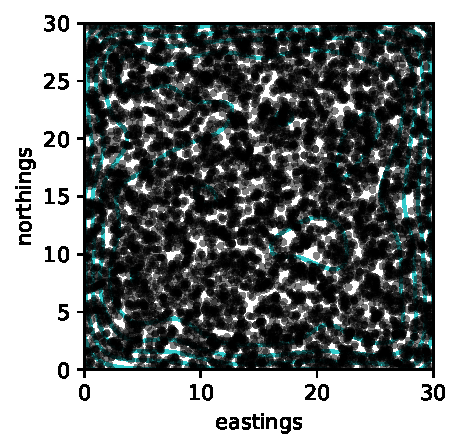
\includegraphics{figures/ex1a/fkpp_123.locations}
        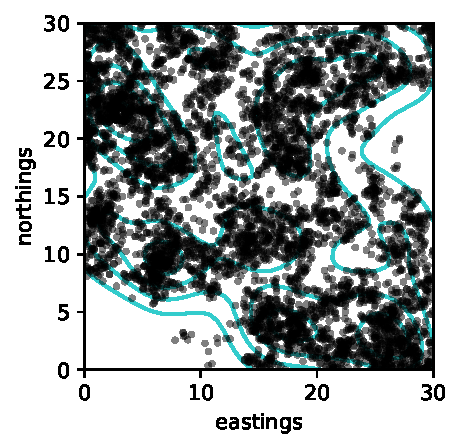
\includegraphics{figures/ex1b/fkpp_123.locations}
    \end{center}
    \caption{
        Snapshots of two simulations, with small $\theta$ (left) and large $\theta$ (right).
        Simulations are run with a FKPP-like parameterization:
        birth and establishment are constant, while death increases linearly with density,
        at slope $1/\theta$.
        Left: $\theta=1$. Right: $\theta=100$.
        Other parameters were the same:
        dispersal and interactions distance were set to 1,
        and the equilibrium density is 10 individuals per unit area.
        \label{fig:super_vs_det_2d}
    }
\end{figure}

\begin{theorem} \label{thm:nonlocal_convergence}
    Let $(\eta^N_t)_{t \geq 0}$
    be as defined in Definition \ref{def:model_setup}
    and assume that as $N \to \infty$, $N \to \infty$
    in such a way that $\theta/N \to \alpha$.
    (However, interaction distances $\epsilon_r$, $\epsilon_\gamma$, and $\epsilon_F$
    remain constant.)

    The sequence of stochastic processes
    $(\eta^N_t)_{t \geq 0}$
    converges along subsequences in distribution as $N \to \infty$
    to a measure-valued process $(\eta_t)_{t \geq 0}$
    which satisfies that, for every $f:\mathbb{R}^d \rightarrow \mathbb{R}$,
    \begin{align} \label{eqn:mgale_problem}
        M_t
        &:=
        \langle f(x), \eta_t(dx) \rangle
        -
        \langle f(x), \eta_0(dx) \rangle
        \\ & \qquad
        -
        \int_0^t \big\langle
            \gamma(x, \smooth{\gamma} \eta_{s}(x))
            \mathcal{B}\left(
                f(\cdot) r(\cdot, \smooth{r} \eta_{s}(\cdot))
            \right)(x)
            +
            f(x)
            F(x, \smooth{F} \eta_{s}(x)),
            \eta_{s}(dx)
        \big\rangle ds,
    \end{align}
    is a martingale.
    The quadratic variation of $M_t$, denoted $\langle M \rangle_t$, is given by 
    \begin{align} \label{eqn:mgale_variation}
        \langle M \rangle_t
        =
        \alpha
        \int_0^t
        \big\langle
            \left(\gamma\left( x,  \eta_{s} \right)
            r\left(x, \eta_{s} \right)+\mu\left(x, \eta_{s} \right)\right)
            f^2(x),
            \eta_{s} (dx)
        \big\rangle ds. 
    \end{align}
    In other words, the limit is a measure-valued process with non-local interactions.
    Furthermore, if $\alpha = 0$ the limit is deterministic.
\end{theorem}

Recall when interpreting~\eqref{eqn:mgale_problem}
that for instance $r(x, \eta_s) = r(x, \smooth{r} \eta_s(x))$,
and so $\DG(fr)(x) = \DG(f(\cdot) r(\cdot, \smooth{r} \eta_s(\cdot)))(x)$.

Theorem \ref{thm:nonlocal_convergence} provided convergence along subsequences;
i.e., for any sequence of values of $\theta$
there is a subsequence that converges.
However, if the limiting process is unique then the convergence is unqualified.
In the deterministic case, we have convergence to a nonlocal PDE.

\begin{corollary}[Superprocess limits] \label{cor:superprocess_uniqueness}
    In the context of Theorem~\ref{thm:nonlocal_convergence},
    if the martingale problem
    defined by equations \eqref{eqn:mgale_problem} and \eqref{eqn:mgale_variation}
    has a unique solution,
    then $(\eta^N(t))_{t \ge 0}$ converges to that solution
    as $N \to \infty$.
    \comment{
        Is this what we want to say here? Could be said better.
        TODO: see what Dawson \& Li say about uniqueness
        so we have at least some conditions under which this happens.
    }
\end{corollary}

Our results will show that in deterministic limits ``$\eta_t$ solves a PDE'',
but since $\eta_t$ is a measure for which we don't always know there exists a density,
we need to formalize the weak sense in which it solves the PDE.
The notation in the following definition
is written to suggest the case in which $\eta_t(dx)$ has a density $\varphi_t(x)$.

\begin{definition}[Weak solutions]
    \label{defn:weak_solutions}
    We say that $(\eta_t)_{t \ge 0}$, with $\eta_t \in \measures$
    is a \emph{weak solution} to the PDE
    $$
        \dot \varphi = r \DG^*(\gamma \varphi) + \varphi F
    $$
    if for all $f \in C_0^\infty(\IR^d)$,
    $$
        \frac{d}{dt} \langle f, \eta_t \rangle
        =
        \langle
            \gamma \DG(rf) + f F,
            \eta_t
        \rangle .
    $$
    \comment{Write this out with $(x)$'s?}
\end{definition}


\begin{corollary}[Deterministic limits]
    \label{cor:nonlocal_pde_limits}
    Under the assumptions of Theorem~\ref{thm:nonlocal_convergence},
    if the limit is deterministic (i.e., $\theta / N \to \alpha = 0$),
    then any limit $\eta_t$ is a weak solution to the nonlocal partial differential equation
    \begin{equation} \label{eqn:nonlocal_pde}
        \partial_t \varphi_t(x)
        =
        r\left(x, \smooth{r} \varphi_t(x) \right)
        \DG^* \left[
            \varphi_t(\cdot)
            \gamma\big( x, \smooth{\gamma} \varphi_t(\cdot) \big)
        \right](x)
        +
        \varphi_t(x)
        F\left(x, \smooth{F} \varphi_t(x) \right)
        ,
    \end{equation}
    in the sense of Definition~\ref{defn:weak_solutions}.
    If equation \eqref{eqn:nonlocal_pde} has a unique solution,
    then $(\eta^N_t)_{t \ge 0}$ converges to that solution.
\end{corollary}

\comment{TODO: find some conditions under which we have convergence to a unique solution?}
\comment{TODO: Tom has conditions (coefficient are Lipschitz?) under which
    the solution to \eqref{eqn:nonlocal_pdf} has a density (Thm 2.1 in DDMOT);
    should we insert those here (as a Corollary or Proposition, maybe?)}

Informally, equation \eqref{eqn:nonlocal_pde} is the PDE
\begin{align} \label{eqn:pde}
    \dot \varphi = r \DG^* \left( \gamma \varphi \right) + \varphi F ,
\end{align}
where $\DG$ is an elliptic second order differential operator,
and the coefficients $r$, $\gamma$, and $F$
at $x$ depend nonlocally on $\varphi$
(i.e., through a smoothed version of $\varphi$).
To see why it is $\DG^*$ and not $\DG$ that appears in this equation,
consider the case where dispersal has a mean drift to the right,
so that the drift term in $\DG$ is $d/dx$.
Then, the population density at a location with positive slope
will tend to \emph{decrease}, i.e., proportional to $-d/dx$,
because the density at a location is determined by the offspring that disperse \emph{to}
that location, not away from it.
Furthermore, if dispersal tends to move offspring away from a region
(i.e., if divergence $\grad \cdot \meanq > 0$)
this will tend to decrease the local density.

Although the coefficients at $x$ in \eqref{eqn:nonlocal_pde} are nonlocal,
they depend only on the region nearby to $x$,
and so we would expect solutions of the nonlocal PDE to be close to the corresponding local PDE
as the interaction distances $\epsilon_r$, $\epsilon_\gamma$ and $\epsilon_F$
go to zero:
for instance, if $\eta_t$ has density $\varphi_t$
then $\gamma(x, \smooth{\gamma} \eta_t(x)) \to \gamma(x, \varphi_t(x))$ as $\epsilon_\gamma \to 0$.
The following propositions give two concrete situations in which that is true.

\begin{proposition}
    \label{prop:nonlocal_to_local}
    Suppose that $\eta^\epsilon_t$ is a weak solution to equation \eqref{eqn:nonlocal_pde}
    with $r(x, m) = 1$ for all $x$ and $m$
    and some $\epsilon_r + 1/\theta < \epsilon_\gamma = \epsilon_F = \epsilon$
    \comment{and assumptions on $\gamma$? and $F$?}.
    Then $\eta^\epsilon_t(dx)$ converges \comment{in what sense?} as $\epsilon \to 0$
    to $\varphi_t(x) dx$, which is a (strong) solution to
    \begin{align} \label{eqn:PDE}
        \partial_t \varphi(t, x)
        =
        \DG^* \left( \gamma(\cdot, \varphi(t, \cdot)) \varphi(t, \cdot)  \right)(x)
        + F(x, \varphi(t, x)) \varphi(t, x) .
    \end{align}
\end{proposition}

Theorem \ref{thm:nonlocal_convergence} combined with Proposition \ref{prop:nonlocal_to_local}
imply that we can take the $N \to \infty$ limit
followed by $\epsilon \to 0$
to obtain solutions to the PDE \eqref{eqn:PDE}.
However, it is of substantial interest to know whether
we can take those two limits simultaneously.
The general case seems difficult,
but we can prove such ``diagonal'' convergence in the following situation.

\begin{theorem}[Convergence to a PDE]
    \label{thm:local_convergence}
    Let $(\eta^N_t)_{t \geq 0}$
    be as defined in Definition \ref{def:model_setup}
    and assume that as $N \to \infty$, $\theta \to \infty$
    and $\epsilon_r + 1/\theta < \epsilon_\gamma = \epsilon_F = \epsilon \to 0$
    in such a way that $\theta/N \to 0$
    and
    \comment{TODO: some conditions on $\epsilon$ and $r$ and $\gamma$ and $F$}.
    Then the sequence of stochastic processes $(\eta^N_t)_{t \ge 0}$
    converges \comment{in some sense}
    to a measure-valued process with a density $\varphi(t, x)$
    that solves
    \begin{align}
        \partial_t \varphi(t, x)
        &=
        \text{whatever the final form is here} .
    \end{align}
\end{theorem}


% % % % % % % % % % % %
\subsection{Main results on lineages}

Now that we have established what we can say about how population density changes with time,
we turn to results on ancestral lineages,
i.e., how genealogical ancestry can be traced back across the landscape.
Informally,
a \emph{lineage} $(L_t)_{t \ge 0}$
begun at spatial location $L_0 = x$
can be obtained by picking a focal individual uniformly at $x$,
and then for each amount of time $t$ in the past,
setting $L_t$ to the spatial location of the individual from whom
the focal individual inherits at that time in the past.
Since in our model individuals have only one parent, this is unambiguous.
Although we did not explicitly retain such information,
it is clear that for finite $N$
one could construct the distribution of a lineage $(L_t)_{t=0}^T$
given the history of the population $(\eta^N_t)_{t = 0}^T$,
for each starting location to which $\eta^N_T$ assigns positive mass.
It is less clear, however, how to formally retain such information in the limit.
The \emph{lookdown construction} in Section~\ref{sec:lookdown}
provides just such a construction,
where lineages are retained in the $N \to \infty$ limit.
Roughly speaking,
this works by assigning to each particle a unique ``level''
that functions as a label and thus allows reconstruction of lineages,
but also (in some sense) orders individuals by eventual reproductive output,
allowing a formal limit.
See~\citet{etheridge/kurtz:2018} for an introduction to these ideas.

A lineage is, in general, a well-defined stochastic process,
but there are two important questions
that affect its tractability.
First, when is it a Markov process given the population process?
(In other words, given $(\eta_t)_{t=0}^T$ that records numbers of individuals
but not their ancestry.)
We expect the answer here to be that a lineage is Markov
only in the $N \to \infty$ limit
(see \citet{barton/depaulis/etheridge:2002} for discussion).
Second, does the process have a tractable description?
If the population process has a density,
then it turns out that a lineage is a diffusion driven by the density.
The remaining case is the superprocess limit ($\theta/N \to \alpha > 0$);
in this case, we expect that a lineage could still be described as a generalized diffusion,
but moving within a stochastic landscape that is singular in $d \ge 2$.
We focus on the more tractable situation where the population process is deterministic.
However, the results here apply to either the local or nonlocal case
(i.e., where the density solves a local or nonlocal PDE).


\begin{definition}[Generator of a lineage] \label{def:lineage_generator}
    Let $(\varphi_t(x))_{0 \le t \le T}$
    denote the density of a population that solves \eqref{eqn:nonlocal_pde},
    and let $y$ be a point with $\varphi_T(y) > 0$.
    We define $(L_s(y))_{s=0}^T$,
    the ancestral lineage in this population of an individual sampled at $y$ at time $T$,
    to be the position of the unique ancestor of $y$ alive at time $T - s$.
    We define
    $(Q_s)_{s \geq 0}$
    to be the time inhomogeneous semi-group satisfying
    \begin{align*}
        Q_s f(y) := \IE_y[ f(L_s) ] .
    \end{align*}
\end{definition}

Our main result identifies a lineage as a diffusion
by characterizing its generator.


\begin{theorem} \label{thm:lineages}
    For $\varphi: \IR^d \to \IR$, define
    \begin{align}
        \label{eqn:lineage_generator}
        \Lgen_\varphi f
        &=
        \frac{r}{\varphi}
        \left[
            \DG^*(\gamma \varphi f) 
            - f \DG^* (\gamma \varphi)
        \right] \\
        &= \label{eqn:lineage_generator2}
        r\gamma
        \left[
            \sum_{ij} \covq_{ij} \partial_{ij} f
            + \sum_j \vec{m}(s)_j \partial_j f
        \right] ,
    \end{align}
    where $\vec{m}$ is the vector
    $$
    \vec{m}(s)_j
    =
    2 \sum_i C_{ij} \partial_i \log(\gamma \varphi)
    + 2 \sum_i \partial_i C_{ij}
    - \meanq_j .
    $$
    Then $\Lgen_{\varphi_{T-s}}$ is the generator of the semigroup $Q_s$
    of Definition~\ref{def:lineage_generator}.
\end{theorem}

As usual,
to make the generator readable, we've written it in concise notation,
omitting the dependencies on location and population density,
which itself changes with time.
When interpreting this,
remember that everything depends on location and density at that location and time --
for instance, ``$r$'' is actually $r(x, \varphi(x))$.

\begin{corollary} \label{cor:lineages_simple}
    In addition to the assumptions of Theorem~\ref{thm:lineages},
    if the dispersal process is isotropic (i.e., $\covq = \sigma^2 I$),
    then
    \begin{equation}
        \Lgen_\varphi f
        =
        \sigma^2 r \gamma
        \left(
            \Delta f
            +
            \left(
                2 \grad \log(\gamma \varphi)
                - \meanq
            \right)
            \cdot \grad f
        \right) .
    \end{equation}
    In other words, 
    a lineage behaves as a diffusion
    that is driven by a Brownian motion 
    run at speed $\sigma^2$ multiplied by the local per-capita production of offspring ($r \gamma$)
    in a potential equal to the local birth output tilted by migration bias
    ($\varphi_s \gamma \exp(-\meanq \cdot x / 2 \sigma^2)$).
\end{corollary}


\begin{corollary} \label{cor:wavefront}
    In addition to the assumptions of Corollary~\ref{cor:lineages_simple},
    suppose that the population process is described by a traveling wave with speed $\wavespeed$,
    i.e., the population has density
    $\varphi(t, x) = w(x - t \wavespeed)$
    where $w$ solves
    \begin{align*}
        r \Delta (\gamma w) + w F + \wavespeed \cdot \grad w = 0 .
    \end{align*}
    Then the semigroup 
    of the motion of a linages in this population 
    $Q_s$ is time-homogeneous with generator
    \begin{align}
        \Lgen f
        &=
        \sigma^2 r \gamma
        \left(
            \Delta f
            +
            2 \grad \log (\gamma w)
            \cdot \grad f
        \right)
        + (\wavespeed - \meanq) \cdot \grad f .
    \end{align}
\end{corollary}


%%%%%%%%%%%%%%%%%%%%%%
\section{Examples and applications}
\label{sec:applications}

Next,
we cover some illustrative examples
and interesting applications.

% % % % % % % % % % % %
\subsection{A nonlinear diffusive population: the Porous Medium Equation}

Consider the porous medium equation (PME) with logistic growth,
\begin{equation}
    \label{eqn:pme}
    \partial_t v = \partial_x^2 (v^2) + v (1 - v) ,
\end{equation}
an example of a reaction-diffusion equation with a nonlinear diffusion term.
Such equations are widely used in a number of contexts in biology in which
it is clear that motility within a population varies with population density.
For example, density dependent dispersal is a common feature in spatial
models in ecology, eukaryotic cell biology, and avascular tumour growth;
see~\cite{sherratt:2010} and references therein for further discussion. 
In particular, it has been suggested as a model for
the expansion of a certain type of bacteria % of the type {\em Paenbacillus dendritiformis}
on a thin layer of agar in a petri dish 
\citep{cohen/golding/kozlovsky/benjacob/ron:1999}. 
We shall pay particular attention to the case in which the equation can be 
thought of as modelling the density of an expanding population. 

Comparing \eqref{eqn:pme} to \eqref{eqn:pde},
we see that to set up a limit in which the population density $\varphi$ follows the PME,
we need $r=1$,
$\gamma = \varphi$, and $F = 1 - \varphi$.
Consulting equation~\eqref{eqn:mu_defn},
this implies that $\mu = (1 + 1/\theta) \varphi - 1/\varphi$.
In other words,
establishment is certain
and birth rates increase linearly with population density,
but to compensate, death rates increase slightly faster (also linearly),
as shown in Figure~\ref{fig:pme_waves}.
Alert readers will notice that
for finite $\theta$ death rates may be negative,
and furthermore rates are not bounded;
in practice we choose a suitably small value for $\beta$ and define
\begin{align*}
    \gamma(x, m) &= (1 - \exp(- \beta m)) / \beta \\
    F(x, m) &= \exp(- \beta m) / \beta ,
\end{align*}
and set $\mu(x, m) = \max(0, \gamma - \theta F)$.
Birth and death rates are equal at density $m = 1$,
corresponding to an unscaled density of $N$ individuals per unit area.

\begin{figure}
    \begin{center}
        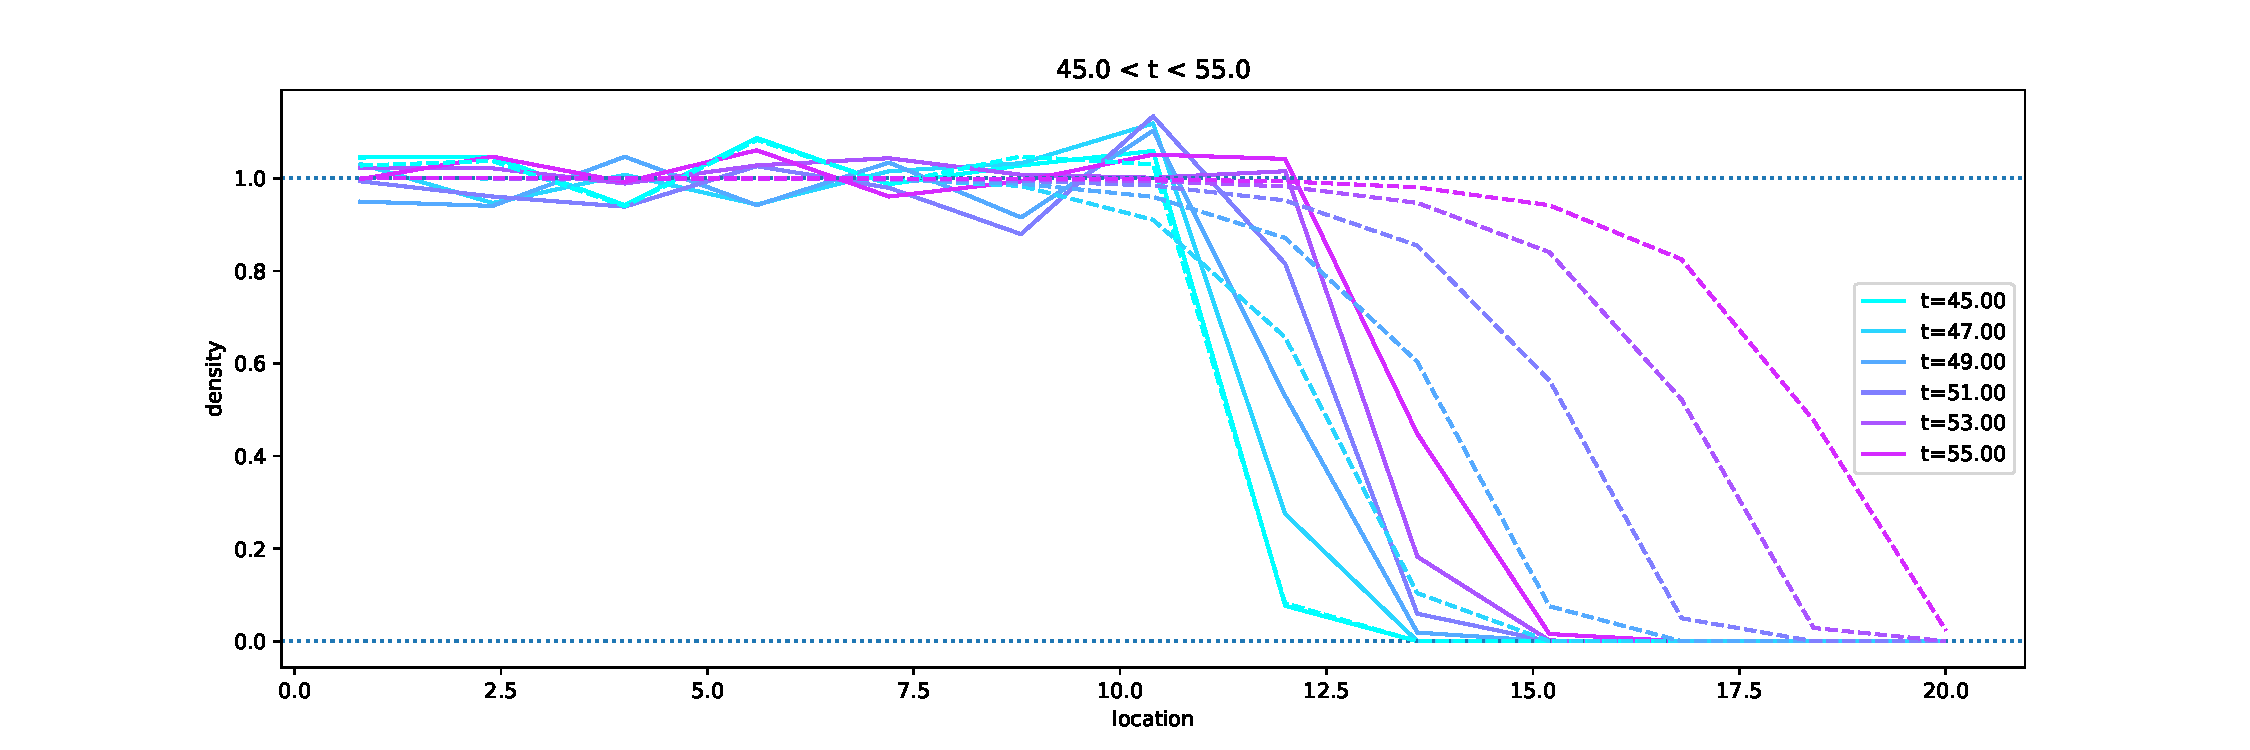
\includegraphics[width=0.45\textwidth]{figures/ex2a/pme_123.steps}
        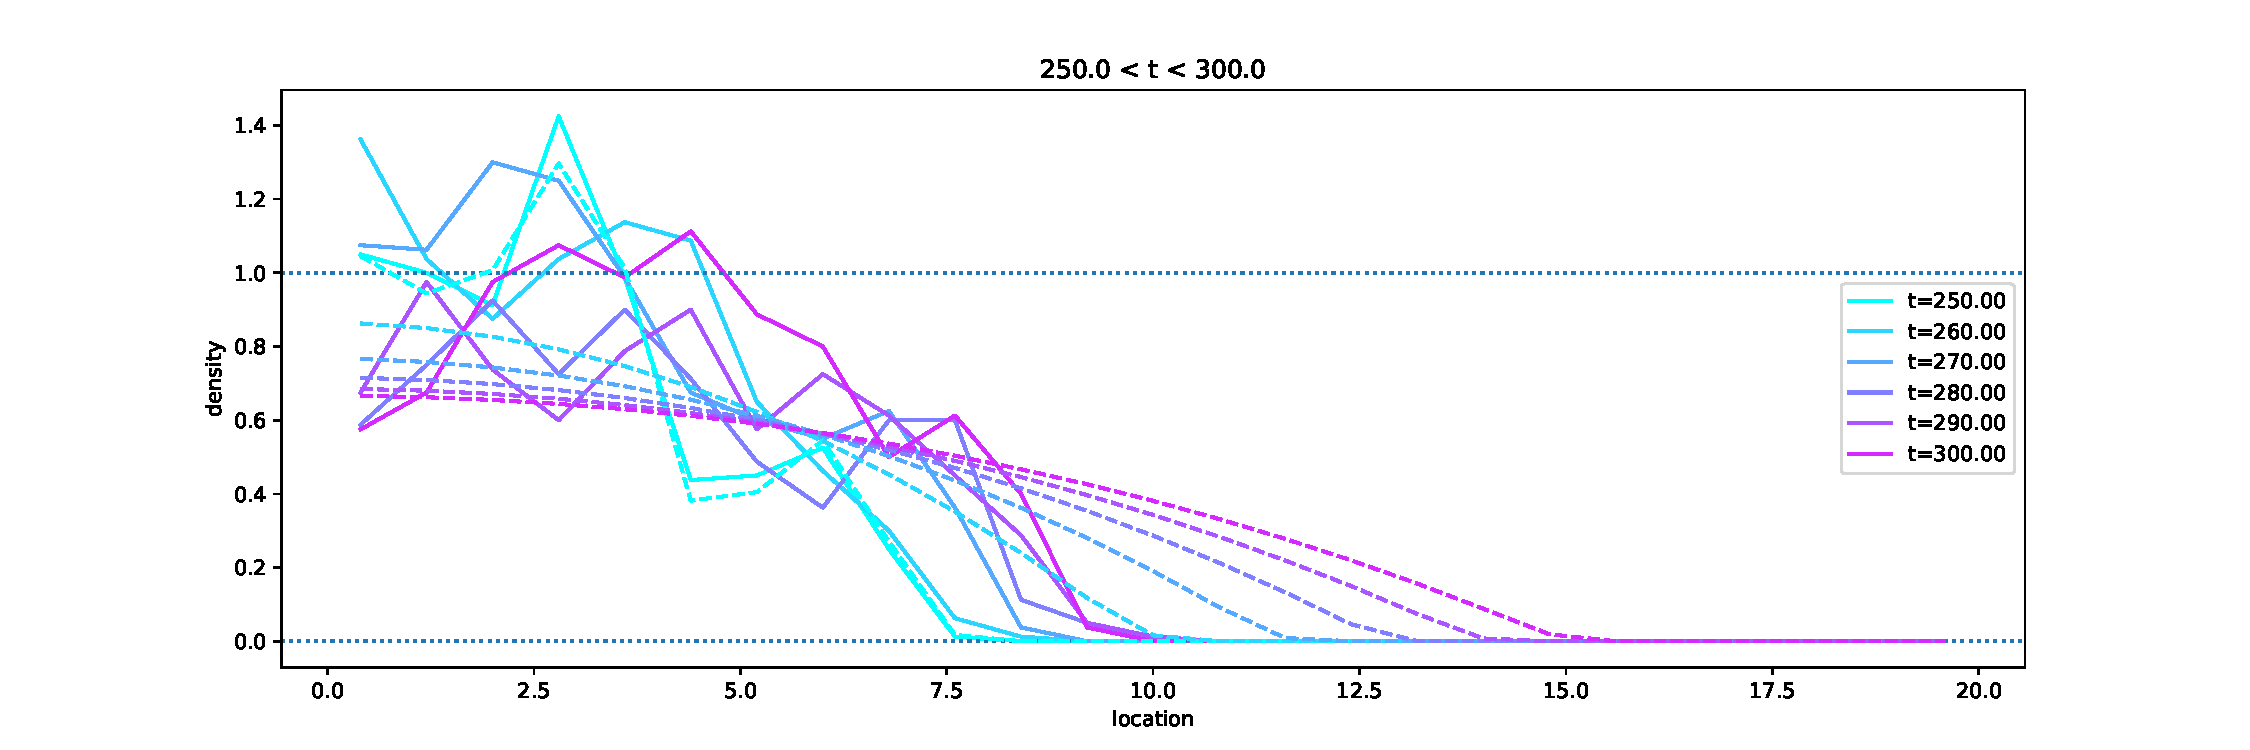
\includegraphics[width=0.45\textwidth]{figures/ex2b/pme_123.steps}
    \end{center}
    \caption{
        Two panels, showing simulated 1D populations under the PME, comparing the simulated
        profile to the analytical solution;
        $\theta/N$ not small on left; small on right.
        (Note: noisier wave should move slower, we'll see this.)
        \label{fig:pme_waves}
    }
\end{figure}

This equation has an explicit travelling wave solution
\begin{align} \label{eqn:pme_wave}
    w^P(t, x)
    :=
    \left( 1 - e^{ \frac{1}{2} (x - x_0 - t) } \right)_+ .
\end{align}
Notice that the wave profile has a sharp boundary at $x = x_0 + t$.
There are also travelling wave solutions with $c>1$ \citep{gilding/kersner:2005},
which lack this property.
However, for initial conditions that decay sufficiently rapidly at infinity,
such as one might use in modelling a population invading new territory,
the solution converges to \eqref{eqn:pme_wave} \citep{kamin/rosenau:2004}.

Indeed, simulations of this process
shown in Figure~\ref{fig:pme_waves}
display traveling wave solutions
similar to numerical solutions of the PME,
with increasingly good agreement for larger $\theta$ and $N$.
As expected, noise slows down the wave.


% % % % % % % % % % % %
\subsection{Traveling waves}

\begin{figure}
    \begin{center}
        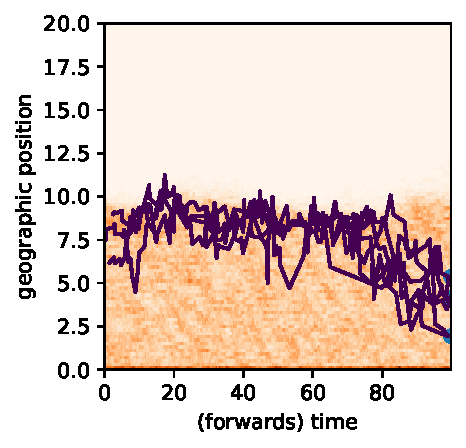
\includegraphics{figures/ex3_fkpp/fkpp_123.lineages}
        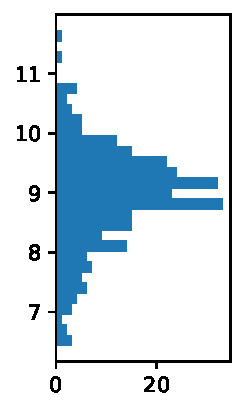
\includegraphics{figures/ex3_fkpp/fkpp_123.lineagehist}
        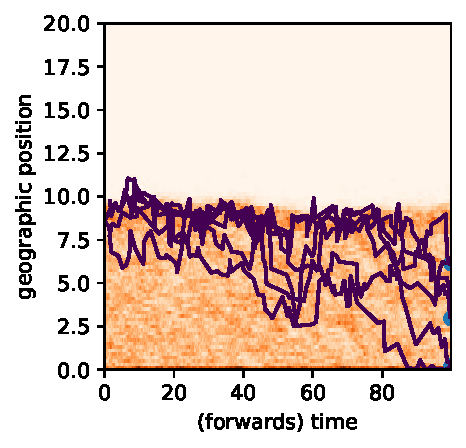
\includegraphics{figures/ex3_pme/pme_123.lineages}
        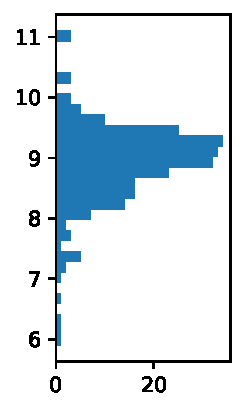
\includegraphics{figures/ex3_pme/pme_123.lineagehist}
        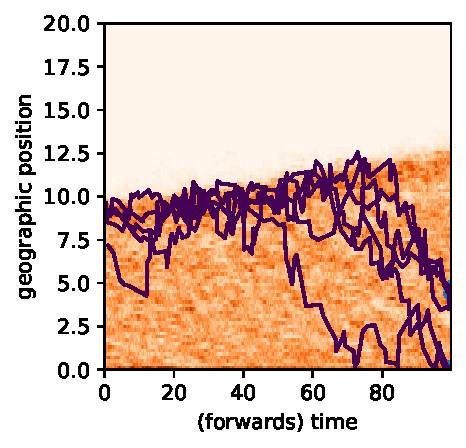
\includegraphics{figures/ex3_allen-cahn/allen-cahn_123.lineages}
        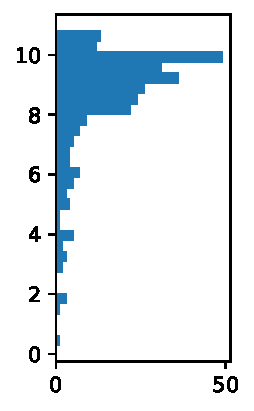
\includegraphics{figures/ex3_allen-cahn/allen-cahn_123.lineagehist}
    \end{center}
    \caption{
        Six panels: one pair for FKPP, one for PME, and one for Allen-Cahn.
        Each pair shows (top) lineage traced back in wavefront,
        and (bottom) stationary distribution of lineage location,
        compared to analytical solution for PME.
        \label{fig:pme_vs_fkpp}
    }
\end{figure}

It is interesting to investigate the motion of an ancestral lineage
in special cases in which we have an explicit expression for the travelling
wave profile $w$. 
We consider three relatively well-studied examples:
the Porous Media equation (above),
the Fisher-KPP equation,
and the Allen-Cahn equation.
We will work here in one dimension,
and take $\sigma^2 = 1$ and $\meanq = 0$.

%%%%%%%%%%
\paragraph{Porous Media:}
Setting $x_0=0$ (for definiteness) and substituting
the form of $w^P$ from equation \eqref{eqn:pme_wave}
into Corollary~\ref{cor:wavefront},
with $c=1$,
$\gamma(x, m) = m$,
$r(x,w) = 1$,
and $F(x, m) = (1 - m)$,
the lineage's generator is, for $x < 0$,
with $f_x$ denoting the spatial derivative of $f$,
\begin{align*}
    \Lgen f
    &=
        w(x)
        \left(
         f_{xx}(x)
         +
         2 \frac{(w(x)^2)_x}{w(x)^2} f_x(x)
        \right)
        + f_x(x) \\
    &=
        \left(1 - e^{\frac{1}{2} x} \right)
        f_{xx}(x)
        -
        2 e^{\frac{1}{2} x} f_x(x)
        +
        f_x(x) .
\end{align*}
The speed measure corresponding to this diffusion is,
again for $x < 0$,
\begin{align*}
    m(d\xi)
    &\propto
        \frac{ 1 }{ 2 (1 - e^{\xi/2}) }
        \exp\left(
            \int_\eta^\xi \left\{
                1 - \frac{e^{x/2}}{1 - e^{x/2}}
            \right\} dx
        \right) \\
    &\propto
        e^\xi\left(1-e^{\xi/2}\right),
        \quad
        \text{for } \xi < 0 ,
\end{align*}
which is integrable and so when suitably normalised gives the unique stationary distribution.
Notice that at stationarity
the lineage will typically be significantly behind the front. 

%%%%%%%%%%
\paragraph{Fisher--KPP:}
A great deal more attention has been paid to the classical Fisher-KPP equation,
\begin{align} \label{eqn:fkpp}
    v_t = v_{xx} + v (1-v) .
\end{align}
Even though we do not have an explicit formula for the wave shape in this case,
our methods provide information about ancestral lineages.
The equation has non-negative travelling wave solutions of speed $c$ for all $c \geq 2$, 
but started from any compact perturbation of a Heaviside function, the 
solution will converge to the profile $w^F$ with the minimal wavespeed, $c=2$,
\cite{kolmogorov/petrovsky/piscounov:1937,bramson:1983}.
No matter the initial condition,
for any $t>0$ the support of the 
solution will be the whole real line. 
In this case, we must have $r = \gamma = 1$,
and $F(x, m) = 1 - m$ so $\mu(x, m) = 1 - (1-m)/\theta$.
This implies that
the generator of the motion of an ancestral lineage is
\begin{equation} \label{eqn:fkpp_generator}
    \Lgen \phi
    =
    \phi_{xx} + 2 \frac{w_x}{w} \phi_x + 2 \phi_x .
\end{equation}
Near the tip of the wave (for $x$ large), $w^F(x) \sim e^{-x}$,
so \eqref{eqn:fkpp_generator} implies that
the motion of a lineage is close to unbiased Brownian motion.
On the other hand, for $x < 0$ a lineage behaves approximately as
Brownian motion with drift at rate two to the right.
This implies that
ancestral lineages are pushed into the tip of the wave,
and there is no stationary distribution,
so that long-term dynamics of genetic inheritance
depend on the part of the wave not well-approximated by a smooth profile.
These results agree with those of \comment{TODO: citations}.


%%%%%%%%%%
\paragraph{Allen-Cahn:}
Finally, we take the Allen-Cahn equation
\begin{align} \label{eqn:allen_cahn}
    v_t = v_{xx} + v(1-v)(2v-1+s),
\end{align}
for a given $s \in (0,2)$,
which is used to model populations evolving under selection \cite{Sarah}.
This equation also has an explicit travelling wave solution with speed $s$
and shape
\[ w^A(x) = (1+e^{x})^{-1}. \]
The generator for ancestral lineages is, just as in the Fisher-KPP case,
\begin{align*}
    \hat{\mathcal{L}}\phi
    &=
    \phi_{xx}
    + 
    2 \frac{w_x}{w} \phi_x
    +
    s \nabla \phi \\
    \qquad &=
    \phi_{xx}
    -
    2 \frac{e^x}{1+e^x} \phi_x 
    + 
    s \nabla \phi,
\end{align*}
so lineages in the tip are pushed leftwards into the bulk of the wave by a $-2(e^{-x}+1)^{-1}$,
that gets weaker further to the left.
This diffusion has speed measure
$$
    m(d\xi) \propto e^{sx}(1+e^x)^{-2},
$$
which is concentrated around $\log(s/(2-s))$ and decays like $e^{x(s-2)}$ away from this point.
These results agree with those of \cite{etheridge/penington:2020}.


% % % % % % % % % % % % % % % %
\subsection{Clumping from nonlocal interactions}

\comment{
    Description of the process;
    discussion of when it happens;
    (TODO: how's it affected by $\theta$?)
}

\begin{figure}
    \begin{center}
        FIGURE
    \end{center}
    \caption{
        Two panels: left is 2D picture of clumped population;
        right is a bumpy expanding wavefront.
        \label{fig:clumping}
    }
\end{figure}


% % % % % % % % % % % % % % % %
\subsection{Nonuniqueness of population density}

It is natural for applications to wonder about identifiability:
when can the observed quantities like population density
or certain summaries of lineage movement uniquely determine
the underlying demographic parameters?
Consider a deterministic,
continuous population generated by parameters $\gamma$, $\mu$, and $r$
with $meanq = 0$ and $\covq = I$.
Suppose it has a stationary profile $w(x)$, that must satisfy
$$
   r \Delta(\gamma w) + (r \gamma - \mu) w = 0 .
$$
It is easy to see that $w$ does not uniquely specify $\gamma$, $\mu$, and $r$:
let $\beta(x)$ be a smooth, nonnegative function on $\IR^d$,
and let $r'(x, m) = \beta(x) r(x, m)$ and $\mu'(x, m) = \beta(x) \mu(x, m)$
(and, let $\gamma' = \gamma$).
Then the population with parameters $\gamma'$, $\mu'$, and $r'$
has the same stationary profile(s) as the original population.

Can these two situations be distinguished from summaries of lineage movement?
The first has lineage generator
\[
    f \mapsto \Lgen f = r \gamma \left( \Delta f + 2 \grad \log(\gamma w) \cdot \grad f \right),
\]
while the second has lineage generator $f \mapsto \beta(x) \Lgen f(x)$.
In other words,
although the stationary profile of the population is unchanged when we scale
local establishment and death by $\beta$,
the motion of lineages is sped up locally by $\beta$.
This corresponds to making areas with $\beta > 1$ more ``sink-like'' and $\beta < 1$ ``source-like'':
if $\beta(x) > 1$, then at $x$ both the death rate and establishment of new individuals are higher.
As a result, lineages in the second model spend more time in areas with $\beta < 1$,
i.e., those areas have higher long-term fitness,
something that is in principle discernible from genetic data.


%%%%%%%%%%%%%%%%%%%%%%%%%
\section{Heuristics}
    \label{sec:heuristics}

In this section we give heuristic arguments for our main results,
to build intuition before the formal proofs.

% % % % % % % % % % % % % % % % % %
\subsection{Population processes}
    \label{sec:population_heuristics}

We write $\Pgen^N$
for the generator of the scaled population process $\eta^N$
of Definition~\ref{defn:mgale_construction}
acting on test functions of the form $F( \langle f, \eta \rangle )$,
where $f \geq 0$ is smooth and compactly supported on $\IR^d$ and 
$F \in C^\infty ([0,\infty))$.
Recall that $\theta \to \infty$ along with $N$,
although we don't remind the reader with extra superscripts.

A Taylor expansion allows us to write
\begin{multline*}
    \Pgen^N
    F(\langle f,\eta \rangle)
    =
    F'(\langle f, \eta \rangle)
    \lim_{\delta t\downarrow 0} \frac{1}{\delta t}
    \IE\left[
        \left. \langle f, \eta_{\delta t} \rangle
        -
        \langle f, \eta \rangle
        \right| \eta_0=\eta
    \right]
    \\
    \qquad {}
    + \frac{1}{2}
        F''(\langle f,\eta\rangle)
    \lim_{\delta t\downarrow 0}\frac{1}{\delta t}
    \IE\left[
        \left.\big(\langle f,\eta_{\delta t}\rangle
        -
        \langle f, \eta\rangle\big)^2 \right|\eta_0=\eta
    \right]
    +
    \epsilon_N(f, F, \eta),
\end{multline*}
where the terms that make up 
$\epsilon_N(f, F, \eta)$
will be negligible in our scaling limit. 

% % % % % % % 
\subsubsection*{Mean measure}

Recall that in our parameterization only death rates $\mu$
and the dispersal kernel $q$ depend on $\theta$.
For a suitable (smooth, compactly supported) test function $f$, we find
\begin{equation} \label{mean measure}
    \begin{split}
    \Pgen^N \langle f, \eta \rangle
    &=
    \lim_{\delta t\downarrow 0} \frac{1}{\delta t}
    \IE\left[ \left.
        \langle f, \eta_{\delta t} \rangle
        -
        \langle f, \eta\rangle
        \right| \eta_0 = \eta
    \right]
    \\
    &=
    \theta \int
        \int f(z) r(z,\eta) q_\theta(x,dz)
    \gamma(x, \eta) \eta(dx)
    -
    \theta \int f(x)\mu_\theta(x, \eta)
    \eta(dx).
    \end{split}
\end{equation}
The first term is the increment in $\langle f,\eta\rangle$
resulting from a birth event (recalling that
we don't kill the parent) integrated against the rate of such events,
and the second reflects death events.
In both terms,
the rate of events has a factor of $N$ (because events happen at a rate 
proportional to the number of individuals,
whereas $\eta$ has mass $1/N$ for each individual)
which is offset by the fact that  
the birth or loss of a single 
individual at the point $y$, say, changes $\langle f,\eta\rangle$
by $f(y)/N$.

We use the fact that $\int q_\theta(x,dz)=1$ to rewrite~(\ref{mean measure})
as 
\begin{equation}
\label{eqn:rewritten mean measure}
\begin{split}
    \int\left(
        \int \theta \left( f(z) r(z,\eta)- f(x) r(x,\eta) \right) q_\theta(x,dz)
    \right)
    \gamma(x,\eta)
    \eta(dx)
    \\
    + \int \int f(x) \theta \Big(
        r(x,\eta) \gamma(x,\eta)
        - \mu_\theta(x,\eta)
    \Big) \eta(dx).
\end{split}
\end{equation}
We have defined $\mu_\theta$ so that the second term is simple:
\begin{align*}
    \theta \Big( r(x,\eta) \gamma(x,\eta) - \mu_\theta(x,\eta) \Big)
    = F(x, \eta) .
\end{align*}
Furthermore, recall from Definition~\ref{def:dispersal_generator} that
\begin{align} \label{eqn:near_critical}
    \int \theta \Big(
        r(z,\eta) f(z)
        -
        r(x,\eta) f(x)
    \Big) q_\theta(x,dz) 
    \qquad \stackrel{\theta\to\infty}{\longrightarrow} \qquad  
    \DG \big(r(\cdot,\Xi)f(\cdot)\big)(x) .
\end{align}
To make this more familiar,
remember that if dispersal is simply standard multivariate Gaussian
with mean zero and covariance $\sigma^2 I / \theta$,
then $\DG = \sigma^2 \Delta$, where $\Delta$ denotes the Laplacian.
Equation~\eqref{eqn:rewritten mean measure}) then converges to
\begin{equation} \label{limit of mean measure equation}
\int \gamma(x,\eta)
\DG \big(f(\cdot)r(\cdot,\eta)\big)(x)
\eta(dx)
+
\int f(x)
F(x,\eta)
\eta(dx) .
\end{equation}
This gives the martingale of Theorem~\ref{thm:nonlocal_convergence}.
More generally, we expect everything to work
if the remaining parameters ($r$, $\gamma$, and $F$)
also depended on $N$, but converged as $N \to \infty$.


% % % % % % % 
\subsubsection*{Quadratic variation}

% Note: this bit in firstversionplus.tex has things written out in detail for
% the Poisson offspring number case.

We now look at the second order term.
An individual at location $x$ gives birth 
to a surviving offspring at $y$ at rate
$$
\gamma(x,\eta) r(y,\eta) q_{\theta}(x, dy) ,
$$
and since this increments $\langle f, \eta \rangle$ by $f(y) / N$,
the contribution to the quadratic variation from birth events,
which occur at rate $\theta$ per individual 
(so, rate $N\theta |\eta|$ overall), is
$$
\langle
    N \theta \gamma(x,\eta)
    \int \frac{1}{N^2} f^2(y) r(y,\eta)
    q_\theta(x,dy) 
    , \eta(dx)
\rangle .
$$
Similarly, the increment in $\langle f, \eta\rangle$ resulting from 
the death of an individual at $x$ is $f(x)/N$, and so combining with the 
above, the second order term in the generator takes the form
\begin{align*}
& F''(\langle f,\eta\rangle)
\frac{1}{2} N \theta
\left\{
    \langle
        \gamma(x,\eta)
        \int \frac{1}{N^2}f^2(y)r(y,\eta)q_\theta(x,dy) 
    , \eta(dx)\rangle
    +
    \langle
        \mu(x,\eta)\frac{1}{N^2}f^2(x) 
    ,\eta(dx)\rangle
\right\} \\
&\qquad
= \frac{1}{2} F''(\langle f, \eta \rangle)
    \frac{\theta}{N}
    \langle
        \gamma(x, \eta) \int f^2(y) r(y, \eta) q_\theta(x, dy) + f^2(x) \mu(x, \eta),
        \eta(dx)
    \rangle .
\end{align*}
Since $\int f^2(y) r(y, \eta) q_\theta(x, dy) \to f^2(x) r(x, \eta)$
and $\gamma r + \mu = 2 \gamma r - F / \theta \to 2 \gamma r$
as $\theta \to \infty$,
this converges to
\begin{align*}
\frac{\alpha}{2} F''(\langle f, \eta \rangle)
    \langle
        2 \gamma(x, \eta) r(x, \eta),
        \eta(dx)
    \rangle .
\end{align*}

Finally, the term $\epsilon_{\theta,N}(f, F, \eta)$ will be 
$\bigO(\theta/N^2)$.

By choosing $\theta/N \rightarrow 0$, the second order term in the generator 
will vanish and we expect a deterministic limit,
for which $d/dt \langle f, \eta_t \rangle$ is equal to~\eqref{limit of mean measure equation}.
In other words, the limit is a weak solution to the deterministic equation
\begin{equation}
\label{deterministic limit}
\frac{d\varrho(x)}{dt}
=
    r(x,\varrho(x))
    \DG\big(
        \gamma(\cdot,\varrho) \varrho(\cdot)
    \big)(x)
    + F(x, \varrho(x)) \varrho(x) 
\end{equation}
in the sense of Definition~\ref{defn:weak_solutions},
where $\varrho_t$ is the density of $\eta_t$, if it has a density.

On the other hand, if $N = \alpha \theta$ for some $\alpha > 0$,
the second order term remains, and we expect a ``generalised superprocess'' limit.
The limiting quadratic variation
is exactly as seen in Theorem~\ref{thm:nonlocal_convergence}.


% % % % % % % % % % % % % % % % % %
\subsection{Lineages}

Although our proof of Theorem~\ref{thm:lineages}
uses the explicit representation in terms of the lookdown process,
informal calculations agree with the main result.
Suppose that we have tracked a lineage to an individual at location $y$ at time $t$.
Looking further back through time, the lineage will move at the time that individual was born,
and will jump to that individual's parents' locations.
Now, the rate at which new individuals are born to parents at $x$ and establish at $y$
is
$$
    \gamma(x, \eta_t) q(x, dy) r(y, \eta_t) .
$$
\comment{TODO: explain this more.}
Happily, we are interested in the case when $\eta$ has a density,
say $\eta_t(dx) = \varphi_t(x) dx$,
so interpreting these rates is not too difficult.
This implies that the probability a randomly chosen individual near $y$
is a new offspring from a parent at $x$ in $[t, t+dt)$ is, informally,
\begin{equation} \label{eqn:informal_rates}
\frac{
    \gamma(x, \eta_t) r(y, \eta_t) \varphi_t(x)
}{
    \varphi_t(y)
} \frac{ q_\theta(x, dy) }{ dy } dx dt .
\end{equation}
Leaving aside questions of whether a lineage can be treated as a randomly chosen individual,
we might then proceed by defining a continuous-time jump process
whose transition rates are given by \eqref{eqn:informal_rates} given $(\varphi_t)_{t=0}^T$.
Let $(L^N_s)_{s=0}^T$ be the location of a lineage that moves according to these jump rates,
back through time (i.e., with the substitution that $s = T-t$).
Then, for the moment writing $q_\theta(x, y)$ for the density of $q_\theta$,
\begin{align} \label{eqn:lineage_generator_Edt}
    \begin{split}
    &\IE[f(L^N_{s+ds}) - f(y) \;|\; L_s = y]
    \\&\qquad 
    =
    ds \int \left(f(x) - f(y)\right)
    \frac{
        \varphi_{T-s}(x) \gamma(x, \eta_{T-s}) r(y, \eta_{T-s})
    }{
        \varphi_{T-s}(y)
    }
    q_\theta(x, y) dx .
    \end{split}
\end{align}
Referring back to Definition~\ref{def:dispersal_generator},
a quick calculation shows that as $N \to \infty$,
\begin{align*}
    \theta \int (f(x) - f(y)) q_\theta(x, y) dx
    &\to
    \DG^* f(x)  - f(x) \DG^* 1 .
\end{align*}
Consequently,
\begin{align*}
    &
    \theta \int (f(x) - f(y)) g(x) q_\theta(x, y) dx \\
    &\qquad =
    \theta \int \left\{
        (f(x) g(x) - f(y) g(y)) - f(y) (g(x) - g(y))
    \right\} q_\theta(x, y) dx \\
    &\qquad \to
        \DG^*(fg)(y) - f(y) \DG^* g(y) . 
\end{align*}
Applying this to~\eqref{eqn:lineage_generator_Edt} with $g = \varphi_{T-s} \gamma$,
this suggests that the generator of the limiting process is
\begin{align} \label{eqn:heuristic_lineage_generator}
    \Lgen_s f
    &=
    \frac{r}{\varphi_{T-s}}
    \left\{
        \DG^*(\gamma \varphi_{T-s} f) - f \DG^*(\gamma \varphi_{T-s})
    \right\} .
\end{align}
This agrees with Theorem~\ref{thm:lineages}.


%%%%%%%%%%%%%%%%%%%
\section{The lookdown process}
    \label{sec:lookdown}

\comment{Should we just use $N$ instead of $\lambda$? Change to $N$ but comment that when comparing ot other papers set $\lambda=N$.}

Now we will present a lookdown construction for the general process
(i.e., of Definition \ref{defn:mgale_construction}),
in the spirit of~\cite{kurtz/rodrigues:2011}. 
The general set-up is as follows.
Each individual will be labeled with a ``level'',
which will be a number in $[0, N]$.
We will still encode the process embellished by these levels
as a point measure:
if the $i^\mathrm{th}$ individual's spatial location is $x_i$
and level is $u_i$, then we will write:
$$
    \lp = \sum_i \delta_{x_i, u_i} ,
$$
which is a measure on $\IR^d \times [0, N]$.
Note that each individual contributes mass 1 to the measure,
not $1/N$ as above.
In some sense, these levels do not affect the process:
the pushforward of this measure-valued ``spatial-level process'',
divided by $N$,
will agree with the purely spatial process defined above.
Furthermore, the levels of the individuals present at any spatial location
are conditionally uniform on $[0, N]$.
However, an individual's level in some sense encodes their future reproductive output:
individuals with lower levels tend to live longer, and have more offspring.
For more explanation of the set-up and how this is possible,
see \citet{etheridge/kurtz:2018} and \citet{kurtz/rodrigues:2011}
(and note that our $N$ corresponds to the $\lambda$ of those papers).
Furthermore, the limiting spatial-level process will still be a point measure,
and so we explicitly retain the notion of individuals and lineages through to the 
large-population-density limit.


% % % % % % % % % % % % % % % %
\subsection{Definition and generator of the lookdown process}
\label{sec:lookdown_defn}

In this section,
we'll define the process $(\lp_t)_{t \ge 0}$ in terms of the dynamics of labeled particles,
and write down its generator.
Since the dynamics depend on the spatial locations of particles,
in this section we define $\eta_t$ to be the corresponding spatial measure,
i.e.,
$$
    \eta_t(\cdot) = \frac{1}{N} \lp_t(\cdot \times [0, N])  .
$$
A nontrivial consequence of the way we define $\lp_t$ will be that
this process has the same distribution as the process $(\eta_t)_{t \ge 0}$ defined above
in Definition~\ref{defn:mgale_construction}.
(This provides our justification for using the same notation for both.)
Finally, note that we first describe the dynamics of individuals
in the original time units -- i.e., before scaling by $\theta$,
which will appear below.

\comment{
    I've defined $\eta = \lp / N$ to agree with how we define the generator below,
    for which birth/death add/remove something of mass 1, not $1/N$.
}

\comment{TODO: this uses the $\gamma(x, \eta)$ notation, which we haven't settled on.}

Suppose that the initial population is composed of $O(N)$ many particles
with levels uniformly distributed between $[0, N]$.
Suppose the current state of the population is $\lp$,
with spatial projection $\eta$.
An individual at spatial location $x$ with level $u$
produces one juvenile offspring at rate 
$$
2 \left(1 - \frac{u}{N}\right) \gamma(x, \eta) ,
$$
which disperses to a location relative to $x$ drawn from the kernel $q(\cdot)$.
(Averaging over the uniform distribution of the level $u$,
we recover the birth rate $\gamma(x, \eta)$.)
This juvenile -- suppose it's location is $y$ --
either survives, with probability $r(y, \eta)$, or immediately dies.
(As before, ``maturity'' is instantaneous.)

A new level $u_1$ is sampled independently and uniformly from $[u,N]$,
and the parent and the offspring are assigned in random order to the levels $\{u, u_1\}$.
This random assignment of levels to parent
and offspring ensures that conditional on $\eta$,
the levels of each individual at any point in time are independent, uniform random variables.

Evidently this mechanism increases the proportion
of individuals with higher levels.
To restore the property that,
conditional on $\eta$,
the distribution of levels is conditionally uniform,
we impose that 
the level of an individual at location $x$
evolves according to the differential equation
$$
    \dot{v}
    =
    % \gamma^{\mathfrak{m}}(x, \eta) \left\{N^{-1}(N -v)^{2} -(N -v)\right\}.
    - \frac{v}{N} \left(N - v\right)
    \gamma(x, \eta) \int_{\IR^d} r(y, \eta) q(x, dy) .
$$
Since $v \in [0, N]$, this moves levels down;
see~\cite{etheridge/kurtz:2018}, Section~3.4 for a detailed explanation.

In the lookdown model, levels never cross below 0,
while particles whose levels move above $N$ are regarded as dead
(and do not affect to the population any more).
Therefore, in order to incorporate death,
the level of the individual at location $x$ with level $u$
moves upwards at an additional rate $\mu(x,\eta) u$.
Since levels are uniform,
it is easy to check that if $\mu$ was constant,
this would imply an exponential lifetime for each individual;
see~\cite{etheridge/kurtz:2018}, Section \comment{TODO}
for more general justification.

Putting these together,
the level $u$ of an individual at $x$ evolves according to:
\begin{equation} \label{eqn:dot_u}
    \dot u
    =
    - \frac{1}{N} u \left(N - u\right)
    \gamma(x, \eta) \int_{\IR^d} r(y, \eta) q(x, dy) 
    +
    \theta \mu(x,\eta) u .
\end{equation}
We shall write 
$$
    b(x, \eta)
    :=
    \theta\left(
    \gamma(x,\eta) \int_{\IR^d} r(y, \eta) q(x, dy)
    -
    \mu(x,\eta)
    \right) ,
$$
which captures the local net difference between reproduction and death,
i.e., the deviation from criticality of the branching mechanism.
Recall from equation \eqref{eqn:mu_defn} that
$F(x,\eta) = \theta(r(x,\eta)\gamma(x,\eta) - \mu(x,\eta))$,
and so we will have that
\begin{align} \label{eqn:b_limit}
\begin{split}
b(x, \eta)
&=
    \theta \gamma(x, \eta) \int_{\IR^d} \left( r(y, \eta) - r(x, \eta) \right) q(x, dy)
    + F(x, \eta) \\
&\to
    \gamma(x, \eta) \DG r(x, \eta) + F(x, \eta) \qquad \text{as } N \to \infty .
\end{split}
\end{align}

We can then rewrite the differential equation 
governing how the level of each individual evolves as
\begin{align}
\dot{u}
    &=
    \gamma(x,\eta) \int_{\IR^d} r(y, \eta) q(x, dy)
    \left\{
        -\frac{u}{N}\left(N - u\right)
        + u
    \right\}
    -
    b(x,\eta) u / \theta
    \nonumber \\
    &=
    \frac{1}{N} \gamma(x,\eta) \int_{\IR^d} r(y, \eta) q(x, dy) u^2
    -
    b(x, \eta) u / \theta
    . \label{differential equation for level}
\end{align}

Now, we can write down the generator for $(\lp_t)_{t \ge 0}$,
the lookdown process.
In what follows, we will write sums (and, products) over ``$(x, u) \in \xi$''
to mean as a sum over the (location, level) pairs of each individual in the population.
Test functions for $\lp$ then take the form
\begin{equation} \label{eqn:test_functions}
f(\lp)=\prod_{(x,u)\in \lp}g(x,u)=\exp\left(\int \log g(x,u)\lp(dx, du)\right),
\end{equation}
where
$g(x,u)$ is differentiable in $u$ and 
smooth in $x$.
We will also assume that $0\leq g(x,u) \leq 1$ for all $u\in [0,N]$,
and $g(x,u)\equiv 1$ for $u\geq N$.
In the expressions that follow,
we shall often see one or more factor of $1/g(x,u)$;
it should be understood that if $g(x,u)=0$,
then it simply cancels 
the corresponding factor in $f(\lp)$.

Recall that just as with $\eta_t$, in defining $(\lp_t)_{t \ge 0}$
we sped up time by a factor of $\theta$.
As a result, per-capita rates below will have a factor of $\theta$
not present in the expressions above.

First consider the terms in the generator that come from birth events.
When a birth successfully establishes,
a new level is generated above the parent's level,
and this new level is assigned to either the offspring or the parent.
Since the probability of each is 1/2,
the contribution of birth to the generator is
\begin{align}
f(\lp) \nonumber
&\mapsto
    f(\lp)
    \sum_{(x, u) \in \lp}
    2 \frac{\theta}{N} \gamma(x, \eta)
    \int_u^N
    \int_{\IR^d}
    \left(
    \frac{1}{2}
    \bigg\{
            g(y, u_1)
        + \frac{ g(y, u) g(x, u_1) }{ g(x, u) }
    \bigg\}
        - 1
    \right)
    r(y, \eta) q(x, dy)
    \\
    \begin{split} \label{eqn:birth_generator}
&=
    f(\lp)
    \sum_{(x, u) \in \lp}
    2 \gamma(x, \eta)
    \bigg\{
        \frac{1}{2 N}
        \int_u^N
        g(x, u_1) du_1
        \frac{
            \theta \int_{\IR^d} (g(y, u) - g(x, u)) r(y, \eta) q(x, dy)
        }{
            g(x, u)
        }
    \\ & \qquad \qquad \qquad {}
        + \frac{\theta}{N}
        \int_u^N \int_{\IR^d}
        \left( \frac{g(y, u_1) + g(x, u_1)}{2} - 1 \right)
        r(y, \eta) q(x, dy)
    \bigg\}
    .
    \end{split}
\end{align}
Here, $u_1$ is the new level and $y$ is the offspring's location,
and so the two terms in the integral correspond to the two situations:
in the first, we have added an individual at $(y, u_1)$,
while in the second, we replace an individual at $(x, u)$
by one at $(x, u_1)$ and another at $(y, u)$.
We've written it in this form because the two pieces
each naturally converge to separate terms in the limit.

The remaining term in the generator is due to the motion of particles' levels:
\begin{align} \label{eqn:level_generator}
    f(\lp)
    \mapsto
    f(\lp)
    \sum_{(x, u) \in \lp}
    \left(
    \frac{\theta}{N}
        \gamma(x,\eta) \int_{\IR^d} r(y, \eta) q(x, dy) u^2
        -
        b(x, \eta)u
    \right)
    \frac{\partial_u g(x,u)}{g(x,u)} .
\end{align}



We can now define the spatial-level process
explicitly as a solution to a Martingale Problem,
whose generator is just the sum of
\eqref{eqn:birth_generator} and \eqref{eqn:level_generator}.

% % % % % % % %
\begin{definition}[Martingale Problem Characterisation]
    \label{defn:lookdown_mgale}
For given positive values of $N$ and $\theta$,
we define $(\lp^{N}_t)_{t \geq 0}$
to be the (unique) solution
to the Martingale Problem
with initial condition $\lp_0 \in \mathcal{M}_F(\mathbb{R}^d \times [0,N])$
and generator $A^{N}$ that satisfies
\begin{equation*}
\begin{split}
& A^{N}f(\lp ) \\
&\quad =
    f(\lp)
    \,\sum_{(x,u)\in \lp}\,
    2 \gamma(x, \eta)
    \Bigg\{ \frac 12 N^{-1}\int_u^N g(x,u_1) du_1
            \times
            \frac{
                \theta \int_{\mathbb{R}^d}
                (g(y,u) - g(x,u))
                r(y, \eta) q_{\theta}(x,dy)
            }{ g(x,u) }
        \\
    &\qquad\qquad\qquad\qquad\qquad\qquad\qquad {} +
        \frac{\theta}{N} \int_u^N
        \int_{\mathbb{R}^d}\left(
            \frac{ g(y,u_1) + g(x,u_1) }{ 2 } - 1
        \right)
        r(y, \eta) q_{\theta}(x,dy)
        du_1
    \Bigg\}\\
    &\qquad\qquad {} +
    f(\lp) \sum_{(x,u)\in\lp}\,
    \left(
        \frac{\theta}{N} \gamma(x,\eta) \int_{\IR^d} r(y, \eta) q_\theta(x, dy) u^2 -b_{\theta}(x,\eta)u
    \right)
    \frac{\partial_u g(x,u)}{g(x,u)}
    ,
\end{split}
\end{equation*}
for all smooth functions $g \in C^{2}_{0}(\mathbb{R}^d)$,
where $f(\lp) = \prod_{(x, u) \in \lp} g(x, u)$ as defined in \eqref{eqn:test_functions},
and $\eta(\cdot) = \lp(\cdot \times [0, N]) / N$ is the scaled spatial pushforward of $\lp$,
as before.
\end{definition}

\comment{I don't think this bit quite makes sense yet without understanding the MMT
section (but, it should be understandable without understanding that section).}

In Appendix \ref{sec: Markov Mapping Theorem Application},
we will show that
if we define $\Gamma (d\textbf{u})$
as the probability kernel that corresponds to
assigning each particle an i.i.d. uniform $[0,N]$-level,
and for any $\lp \in \mathcal{M}_f(\mathbb{R}^d \times [0,\infty))$, we denote
$$\hat{f}(\lp)=\int f(\lp) \Gamma (d\textbf{u})$$ 
to be the spatial test functions with averaged level,
then the process
\begin{equation}
\begin{aligned}
M^{N}_t:=&\hat{f}(\lp_t)-\hat{f}(\lp_0)-\int_{0}^{t}\int   A^{N}f(\lp_s)\Gamma(d\textbf{u})ds\\
:=&\hat{f}(\lp_t)-\hat{f}(\lp_0)-\int_{0}^{t}   \Pgen^{N}\hat{f}(\lp_s)ds
\end{aligned}    
\end{equation}
is a martingale.

By the Markov Mapping Theorem,
there exists a solution $(\lp^{N}_t)_{t \geq 0}$
to the Martingale Problem with generator $A^{N}$.
Furthermore,
the spatial projection of $(\lp^{N}_t)_{t \geq 0}$
shares the same law of $(\eta^{N}(t))_{t \geq 0}$,
i.e.
$$(\eta^{N}(t))_{t \geq 0}
\sim \left(\frac{1}{N}\sum\limits_{(X(t),U(t))\in \lp^{N}(t)} \delta_{X(t)}\right)_{t \geq 0},$$
and conditional on 
$(\eta^{N}(t))_{t \geq 0}$,
the levels of particles in $(\lp^{N}_t)_{t \geq 0}$
are i.i.d. uniformly distributed between $[0,N]$.

Theorem A.10 in \cite{kurtz/rodrigues:2011}
states that convergence of $(\eta^{N}_t)_{t \geq 0}$
to a conditionally Poisson system $(\lp_t)_{t \geq 0}$
with Cox measure $\eta_t \times \Lambda$
is equivalent to convergence of
$(\eta^{N}_t)_{t \geq 0}$ to $(\eta_t)_{t \geq 0}$.
As a result, it suffices for us to focus on
tightness of $(\eta^{N}_t)_{t \geq 0}$
and spatial convergence of $(\eta^{N}_t)_{t \geq 0}$
as $N \to \infty$.


%% %% %% %% %% %% %% %% %% %% %% %%
\subsection{Construction tracking individual lines of descent} \label{sec: individual lines of descent}

Although in Section \ref{sec:proofs} we will show convergence of the lookdown process
defined by Definition~\ref{defn:lookdown_mgale}
to a stochastic process in which individuals retain their identities,
it is convenient to construct the lookdown process
in a way that explicitly represents the motion of each individual and their offspring.
This will then make obvious how lineages move in the limit,
and will allow us to identify all 
individuals in the current population that are descendants of a
given ancestor at time zero. In theory at least, this allows us to
recover all the information about genealogies relating individuals 
sampled from the present day population. This idea draws on the notion
of `tracers', popular in statistical physics and used in population
genetics by a number of authors including 
\cite{biswas/etheridge/klimek:2018, durrett/fan:2016, hallatschek/nelson:2008}.

We will construct the process using a Ulam-Harris indexing scheme,
which associates the outcomes of each branching event with a label obtained
by appending to the previous label.
To begin, we assign each extant individual a label from $\IN_{\ge 0}$.
Suppose an individual with label $a$ and level $u$ reproduces,
and as a result there are two individuals, one with level $u$ and one with a new level $u_1 > u$.
The parent individual, previously labeled $a$, might be assigned either level.
We will track chains of descendant individuals forwards through time
following levels, rather than individuals, and will call this a \emph{line of descent}.
So, after reproduction, we give a new label to \emph{only} the individual
that is given the new level $u_1$,
retaining the label $a$ for the individual with the old level $u$.
So, there is a unique label assigned at each birth event,
and it is assigned to the resulting individual with the higher level.
It would be possible to reconstruct individual identities along a line of descent
from this construction,
but we don't write this out.

Concretely, then: for each label $a$ in
$\labelspace = \bigcup_{k \ge 1} \IN_{\ge 1}^k$
let $\Pi_a$ be an independent Poisson process on $[0, \infty)^2 \times \IR_d \times \{0,1\}$.
The mean measure is a product of Lebesgue measure on the first two coordinates,
$q(0, \cdot)$ on $\IR^d$, and $(\delta_0 + \delta_1)/2$ on $\{0, 1\}$.
It will also be convenient
to suppose that for each label $a$ we have an enumeration of the points in $\Pi_a$,
so we may refer to ``the $j^\text{th}$ point in $\Pi_a$'',
although the precise order of this enumeration is irrelevant.
If $(t, v, y, \kappa)$ is the $j^\text{th}$ point in $\Pi_a$,
then $t$ will determine possible birth times,
$v$ will determine levels of the offspring,
$y$ will give the spatial displacement of the offspring relative to the parent,
$\kappa$ will be used to determine whether parent or offspring are assigned the new level,
and the new label produced will be $a \concat j$,
i.e., the label $a$ with $j$ appended (so, if $a \in \IN_{\ge 0}^k$ then $a \concat j \in \IN_{\ge 0}^{k+1}$).
Each label $a$ has a birth time $\tau_a$,
when it is first assigned,
and a death time $\sigma_a$, when its level first hits $N$.
For any $\tau_a \le t \le \sigma_a$ we denote by $X_a(t)$ and $U_a(t)$ the spatial location and level
of the individual carrying label $a$ at time $t$.
Now, since we have defined labels so that the level does not jump,
$U_a$ satisfies~\eqref{eqn:dot_u} for $\tau_a \le t \le \sigma_a$, i.e.,
\begin{equation} \label{eqn:U_line_of_descent}
    \begin{split}
& U_a(t)
    =
    U_a(\tau_a) \\
&\qquad {}   
    + \int_{\tau_a}^{t}
    \left(
        \frac{\theta}{N} \gamma(X_a(s),\eta_s)
        \int_{\IR^d} r(z,\eta_s) q(X_a(s),dz) U_a(s)^2
        -
        b(X_a(s),\eta_s) U_a(s)
    \right)
    ds ,
\end{split}
\end{equation}
and, of course, $\sigma_a = \inf\{t \ge \tau_a : U_a(t) > N\}$.

Potential reproduction events occur at times $\tau_a + s$
for each point $(s, v, y, \kappa) \in \Pi_a$.
We say `potential' since if the resulting level is greater than $N$,
the event does not happen.
If this is the $j^\text{th}$ point in $\Pi_a$,
the new label is $a \concat j$, the (potential) birth time is $\tau_{a \concat j} = \tau_a + s$.
For convenience define
$$
    \ell(x, y, \eta, v)
    =
    \frac{
        v
    }{
        2 N^{-1} \theta \gamma(x, \eta) r(x + y, \eta)
    } ,
$$
and using this, the (potential) new level is
\begin{equation*}
    U_{a \concat j}(\tau_{a \concat j})
    =
    U_a(\tau_{a \concat j})
    +
    \ell(X_a(\tau_{a \concat j}-), y, \eta(\tau_{a \concat j}-), v) .
\end{equation*}
If $U_{a \concat j}(\tau_{a \concat j}) < N$,
the new individual labeled $a \concat j$ is produced,
and $\kappa$ determines which label is associated with the new location,
so
\begin{align*}
    X_{a \concat j}(\tau_{a \concat j})
    &=
    X_a(\tau_{a \concat j}-) + (1 - \kappa) y .
\end{align*}
On the other hand
if $U_{a \concat j}(\tau_{a \concat j}) \ge N$, then $X_a$ is unchanged and $X_{a \concat j}$ is undefined,
so
\begin{align} \label{eqn:X_line_of_descent}
    X_a(\tau_{a \concat j})
    &=
    X_a(\tau_{a \concat j}-) + \kappa y \ind_{U_{a \concat j}(\tau_{a \concat j}) < N} .
\end{align}
Recall that the parental \emph{individual} always retains their spatial location,
so that $\kappa = 0$ corresponds to the parent being assigned a new level,
and our line of descent switching to the offspring.

Although we have described the evolution of a line of descent only for a given label
(i.e., for $\tau_a \le t < \sigma_a$),
we can extend the definition to earlier times
by setting for $0 \le t < \sigma_a$
$X_a(t)$ equal to $X_{[a]_t}(t)$,
where $[a]_t$ is the label of the ancestor of label $a$ alive at time $t$,
and similarly for $U_a(t)$.
It is then straightforward, albeit tedious,
to write down the time evolution of $(X_a(t), U_a(t))$ for all time back to $t=0$
in terms of the driving Poisson processes.
Although at finite $N$ the spatial process $X_a(t)$ is affected by jumps in the level $U_a(t)$,
we will see that in the $N \to \infty$ limit
the behavior of $X_a(t)$ is not affected by these jumps.


We can now express the population processes using these levels:
\begin{align*}
    \eta^N_t = \frac{1}{N} \sum_{a : \tau_a \le t < \sigma_a} \delta_{X_a(t)}
    \qquad \text{and} \qquad
    \lp^N_t = \sum_{a : \tau_a \le t < \sigma_a} \delta_{(X_a(t), U_a(t))} .
\end{align*}


\subsubsection{Evolution of levels along a whole line of descent}
We now write down expressions
that give the spatial and level dynamic
of a whole line of descent.
In particular, our description is consistent
for any $N \in \mathbb{N}$.

Recall that
the particle with label $(a_0,a_1,..,a_k)$
is the offspring
with a new level
from the $a_k$-th potential birth
of $(a_0,...,a_{k-1})$,
who is again the offspring
with a new level from
the $a_{k-1}$-th potential birth
of $(a_0,...,a_{k-2})$, 
etc..
In particular, 
the particle with label $(a_0)$
is the direct descendant of
the $a_0$-th original ancestor
of the whole population, i.e.
it has never experienced
a jump in level throughout
its ancestry.

For simplicity, for $a=(a_0,..,a_k)$,
we denote $[a]_{i}:=(a_0,..,a_i)$
to be the $i$-th generation 
ancestor of the lineage $a$.
In particular, if at time $t$,
if the ancestral lineage $[a]_t$
is at its $i(t)$-th generation,
then $[a]_t = [a]_{i(t)}$.

We also write 
$(s_{[a]_{i}}, v_{[a]_{i}}, y_{[a]_{i}}, \kappa_{[a]_{i}})
\in \Pi_{[a]_{i-1}}$
to be the reproduction event
that creates $[a]_{i}$ from $[a]_{i-1}$,
and similarly,
$(s_{[a]_{i} \concat j}, v_{[a]_{i} \concat j}, y_{[a]_{i} \concat j}, \kappa_{[a]_{i} \concat j})
\in \Pi_{[a]_{i-1}}$
to be the reproduction event 
that creates $[a]_{i} \concat j$
from $[a]_{i-1}$.

We first write down an expression
for the level of particle $a=(a_0,a_1,..,a_k)$ at time $t$.
Since we ensure that
the level of a particle
only jumps when a reproduction event
creates a new label,
the level of particle $a=(a_0,a_1,..,a_k)$ is determined
by $k$ many jumps,
and subsequent continuous evolutions
given by Equation \eqref{eqn:U_line_of_descent}.



Under this notation, for $t> 0$,
\begin{equation}
\label{eq: level_across_lineage}
\begin{aligned}
&U^{N}_{[a]_{k}}(t)- U^{N}_{[a]_{0}}(0)\\
=& \sum_{i=1}^{k} \int_{\tau_{[a]_{i-1}}}^{\tau_{[a]_{i}}}
\left(
        \frac{\theta}{N} \gamma(X_{[a]_{i-1}}(s),\eta_s)
        \int_{\IR^d} r(z,\eta_s) q(X_{[a]_{i-1}}(s),dz) U_{[a]_{i-1}}(s)^2
        -
        b(X_{[a]_{i-1}}(s),\eta_s) U_{[a]_{i-1}}(s)
    \right)
    ds\\
&+\int_{\tau_{[a]_{i}}}^{t}
\left(
        \frac{\theta}{N} \gamma(X_{[a]_{i}}(s),\eta_s)
        \int_{\IR^d} r(z,\eta_s) q(X_{[a]_{i}}(s),dz) U_{[a]_{i}}(s)^2
        -
        b(X_{[a]_{i}}(s),\eta_s) U_{[a]_{i}}(s)
    \right)
    ds\\
&+\sum_{i=1}^{k}
    \left( \ell(X_{[a]_{i-1}}(\tau_{[a]_{i}}-), y_{[a]_{i}}, \eta(\tau_{[a]_{i}}-), v_{[a]_{i}})
    \right)
\end{aligned}    
\end{equation}
where the first two terms correspond to
sum of the evolution along the same generation,
and the second term corresponds
to the sum of jumps in levels
when a new label is introduced.

To preserve consistency 
as we send $N \to \infty$
in our scaling limit,
we allow $U_{[a]_t}(t)$ to hit $\infty$.
To identify dead lines of descent,
for a label $a$,
we define
$\sigma_{a}^{N}:= \inf\{t \geq 0 : U_{[a]_t}(t) > N\}$.
In the $N$-th scaling regime,
we proclaim the individual
$a$ to be dead
at time $t$
when $t > \sigma_{a}^{N}$

Note that in particular,
if $U_{[a]_i}(t)>N$
at some time $t$
in the $i$-th generation,
then $U_{[a]_j}(t)>N$
for all $j \geq i$
and
$\sigma_{[a]_j}^{N}=\sigma_{[a]_i}^{N}$.
In words, all descendants of dead
particles are dead by default.

Similarly, we generalise the notion of death above
to the infinity case by considering 
$\sigma_{[a]_t}^{\infty}:=\inf\{t \geq 0 : U_{[a]_t}(t) =\infty\}$.

\subsubsection{Spatial jumps along a whole line of descent}

We now write down an expression for the
spatial location of $[a]_t$ at time $t$.
Note that in the spatial case,
jumps occur along the same generation
whenever $\kappa = 0$ in successful birth events,
and occur across two generations
whenever $\kappa = 1$ in successful birth
events.

To illustrate this, consider the spatial location of $(a_0,a_1)=(2,3)$ with birth time $\tau_{(2,3)}$ at some time $t>\tau_{(2,3)}$.
If $U_{(2,1)}(\tau_{(2,1)}) < N$,
the first birth event of the ancestor
with label $(2)$
is successful.
If $\kappa = 0$ in this birth event,
the parent and offspring swap labels,
resulting in
a spatial jump for the label $(2)$.
On the contrary, 
if $U_{(2,2)}(\tau_{(2,2)}) \geq N$
or $\kappa = 1$
in the second birth event of $(2)$,
the parent does not give birth
or retains its label,
so there is no spatial jump.

On the other hand, 
if $\kappa=1$ when $(2,3)$ is born,
the new label is given to
the offspring
with new spatial location,
resulting in a jump,
and vice versa.

After $(2,3)$ is born,
whenever the particle with label
$(2,3)$ gives birth, 
if $\kappa = 0$, the label $(2,3)$
is adopted by the offspring
which results in a spatial jump
in the position of $(2,3)$
again.

Under this notation, for $t>\tau_{[a]_k}$,


\begin{equation}
\label{eq: space_across_lineage}
\begin{aligned}
&X^{N}_{[a]_{k}}(t)- X^{N}_{[a]_{0}}(0)\\
=& \sum_{i=1}^{k}
\sum_{j=1}^{a_i-1}
(1-\kappa_{[a]_{i-1}\concat j}) y_{[a]_{i-1}\concat j} \ind_{U_{[a]_{i-1}\concat j}(\tau_{[a]_{i-1}\concat j}) < N}\\
&+ \sum_{i=1}^{k}
\kappa_{[a]_i} y_{[a]_i} \ind_{U_{[a]_i}(\tau_{[a]_i}) < N}\\
&+\int_{\tau_{[a]_k}}^{t}
(1-\kappa)y
\ind_{ \{
        U_{[a]_k}(\tau_{[a]_k}+s)
        +\ell(X_{[a]_k}(\tau_{[a]_k}+s),y,\eta_{[a]_k}(\tau_{[a]_k}+s),v) < N
        \}
      } 
\Pi_{[a]_k}(dsdvdyd\kappa),
\end{aligned}    
\end{equation}
where the first term
corresponds to 
the sum of $a_{i}-1$ many potential jumps
in the $(i-1)-th$ generation;
the second term corresponds to 
the sum of $k$ many potential jumps
when the $k$-th generation is introduced;
and the last term
corresponds to sum of 
potential jumps that occured in
the current generation from 
time $\tau_{[a]_k}$
to current time $t >\tau_{[a]_k}$.


%% %% %% %% %% %% %% %% %% %% %% %%
\subsection{Limiting processes for lines of descent}
\label{sec:limiting_lines_of_descent}

The previous section constructs the lookdown process
in a way that makes individual lines of descent converge pointwise as $N \to \infty$,
using the same underlying Poisson processes $\{\Pi_a\}_{a \in \labelspace}$.
To see this, first note that if the Poisson processes are fixed
then the set of events to which a given label $a \in \labelspace$ is associated
is also fixed -- this is the sequence $(s_k, v_k, y_k, \kappa_k)$ associated with a given label $a$.
Therefore, the processes $\Gamma_a$ are also unchanged.
First, we clearly need that the spatial projections $\eta$ converge.

Supposing that they do,
consider how a line of descent $(X_a(t), U_a(t))$ evolves.
The line of descent throws off a new line of descent at a higher level
when there is a point $(s, v, y, \kappa)$ in $\Pi_a$ with 
\begin{equation} \label{eqn:line_points}
    v < 2 (N - U_a(\tau_a + s)) N^{-1} \theta \gamma(X_a(\tau_a + s), \eta_{\tau_a + s}) r(X_a(\tau_a + s)+y, \eta_{\tau_a + s}) .
\end{equation}
Since the mean measure of the $v$ coordinate is Lebesgue,
$\theta/N \to \alpha$,
and $q(x, dy) \to \delta_x(dy)$,
this corresponds in the limit to new lines of descent being thrown off at all times,
i.e., according to a Poisson process with rate
$$
2 \alpha \gamma(X_a(t), \eta_{\tau_a + s}) r(X_a(t), \eta_{\tau_a + s}) 
$$
and uniform intensity on higher levels.
Again, since in the limit the dispersal distance is zero,
new levels are produced at the same spatial location.
However, this affects the location of the line of descent:
for each new line of descent, there is a $1/2$ chance
that the line of descent switches location (i.e., moves to $X_a(t) + y$).
Taking $g$ to be a suitable test function on $\IR^d$, 
and rewriting~\eqref{eqn:line_points},
the generator of this motion is, when the level is $u$
and the state of the population is $\eta$,
\begin{align*}
    g(x)
    &\mapsto
    \left(1 - \frac{u}{N}\right) \gamma(x, \eta)
    \theta \int_{\IR^d} r(x+y, \eta) (g(x+y) - g(x)) q(x, dy) \\
    &=
    \left(1 - \frac{u}{N}\right) \gamma(x, \eta)
    \bigg\{
        \theta \int_{\IR^d} (r(x+y, \eta) g(x+y) - r(x, \eta) g(x)) q(x, dy) \\
        &\qquad \qquad {}
        -
        \theta \int_{\IR^d} (r(x+y, \eta) - r(x, \eta) ) g(x) q(x, dy) 
    \bigg\} \\
    &\to
    \gamma(x, \eta)
    \left(
        \DG(rg)(x) - g(x) \DG(r)(x)
    \right) .
\end{align*}
Notice that the factors of 2 have canceled,
and that the result is independent of $u$.

The only thing that remains is to describe how the levels change,
but this is immediate from applying equation~\eqref{eqn:b_limit}
to equation~\eqref{differential equation for level}.

To write out the joint motion of spatial coordinate and levels,
it is useful to work out the differential operator above in more detail.
Recall that $\DG g(x) = \sum_i \meanq_i \partial_i g(x) + \sum_{ij} \covq_{ij} \partial_{ij} g(x)$,
and for the moment write $r(x)$ for $r(\cdot, \eta(\cdot))(x)$,
so that
\begin{align}
\DG(rg)(x) - g(x) \DG(r)(x)
    &= \nonumber
    r(x) \sum_i \meanq_i \partial_i g(x)
    + 2 \sum_{ij} \meanq_i \partial_i r(x) \covq_{ij} \partial_j g(x)
    + r(x) \sum_{ij} \covq_{ij} \partial_{ij} g(x) \\
    &= \label{eqn:limiting_generator}
    r(x) \left\{
        \left(
        \meanq
        + 2 \covq \grad \log r(x)
        \right)
        \cdot
        \grad g(x)
        +
        \sum_{ij} \covq_{ij} \partial_{ij} g(x)
    \right\} .
\end{align}

We summarize the results in a proposition.

\begin{proposition}[Line of descent construction]
Let $\beta(x, \eta) = \meanq + 2 \covq \grad \log r(x, \eta)$
and $K$ such that $\covq = K K^T$.
Associate with each label $a \in \labelspace$
an independent $d$-dimensional Brownian motion $W_a$
and an independent Poisson process $R_a$ on $[0, \infty)^2$
with Lebesgue mean measure,
as before with points ordered in some way.
Given $\eta_0 \in \measures$,
let $(x_i, u_i)$ be the points of a Poisson process
with mean measure on $\IR^d \times [0, \infty)$ a product of $\eta_0$ and Lebesgue measure.
For each point begin a line of descent
with label $i$, location $X_i(0) = x_i$, level $U_a(0) = u_i$, and birth time $\tau_i = 0$.
Suppose that the spatial locations and level of each line of descent $a$
behave, for $\tau_a \le t < \sigma_a$ as, as
\begin{align*}
X_a(t)
    &=
    X_a(\tau_a)
    + \int_{\tau_a}^{t}
    \bigg(
        \beta(x, \eta(s)) ds
        +
        K dW_a(s)
    \bigg)
    ds  \\
U_a(t)
    &=
    U_a(\tau_a)
    + \int_{\tau_a}^{t}
    \bigg(
        \alpha \gamma(X_a(s),\eta(s))
        r(x,\eta(s)) U_a(s)^2
\\ &\qquad \qquad \qquad {}   
        -
        \left\{
            \gamma(X_a(s),\eta(s)) \DG r(X_a(s),\eta(s))
            + F(X_a(s), \eta(s))
        \right\}
        U_a(s)
    \bigg)
    ds .
\end{align*}
Each point in the $R_a$ denotes a potential birth time for $a$:
if the $j^\text{th}$ point in $R_a$ is $(t, v)$, with $t < \sigma_a - \tau_a$,
then a new line of descent with label $a \concat j$ is produced,
with birth time $\tau_{a \concat j} = \tau_a + t$,
location $X_{a \concat j}(\tau_a + t) = X_a(tau_a + t)$, and level
$$
    U_{a \concat j}(\tau_a + t) = U_a(\tau_a + t)
    + \frac{v}{ 2 \alpha \gamma(X_a(\tau_a + t), \eta_{\tau_a + t}) r(X_a(\tau_a + t), \eta_{\tau_a + t}) } .
$$
For each $a$, let $\sigma_a = \inf\{t \ge 0: U_a(t) < \infty\}$.
Then, the processes defined by
\begin{align*}
    \eta_t = \lim_{N \to \infty} \frac{1}{N} \sum_{a : \tau_a \le t < \sigma_a} \delta_{X_a(t)}
    \qquad \text{and} \qquad
    \lp_t = \sum_{a : \tau_a \le t < \sigma_a} \delta_{(X_a(t), U_a(t))} 
\end{align*}
agree in distribution with those of Definitions~\ref{defn:mgale_construction} and~\ref{defn:lookdown_mgale},
respectively.
\end{proposition}




%%%%%%%%%%%%%%%%%%%%%%%%%%
\section{Proofs}
\label{sec:proofs}

\comment{
    TODO: write overview.
    To prove convergence, we'll be proving
    (a) tightness
    (b) convergence of generators, and
    (c) uniqueness of the limit.

    Then, to get convergence of the lookdown
    we use the population process (somehow).
}

\begin{proof}[Proof of Theorem~\ref{thm:nonlocal_convergence}.]

\comment{INSERT HERE
    narrative of tightness,
    proved in Section \ref{sec:population_tightness_proofs},
    and convergence of generators,
    proved in Section \ref{sec:population_generators_proofs}.
}

\end{proof}


% % % % % % % % % % % % %
\subsection{Tightness of empirical measures}
    \label{sec:population_tightness_proofs}
To prove tightness of our population process, 
we first show that the expected total mass of our population process at some fixed time $T>0$,
is controlled uniformly across $\theta$.
This is equivalent to the compact containment condition.

To establish this control,
we first prove a technical lemma which controls spatial density of our population,
and then we use the BDG inequality on a martingale
to give us control over the running supremum of our total population mass.

Once we have control over the total mass of the population, 
we will also have control over local densities.
This then allows us to prove that the particle system is tight
by an application of the Aldous-Rebelleon Criterion.

\subsubsection{Compact Containment Condition}
Before proving compact containment condition,
we first prove a technical lemma that involves a bound on the Gaussian kernels.
\begin{lemma}
    \label{lem: gamma - r radius comparison}
    Assume that $\epsilon_{r}^2 + \frac{1}{\theta} < \epsilon_{\gamma}^2,$ then
    for all $f \in \mathcal{C}^{2}_{0}(\mathbb{R}^d \times \mathbb{R})$
    with bounded first and second derivatives
    and for all $\eta \in \mathcal{M}_{f}(\mathbb{R}^d)$, we have 
    
    \begin{equation}\label{eq: gamma - r radius comparison bound}
    \gamma\big(x,\rho_{\gamma}*\eta(x)\big)
    \left| \theta 
        \int_{\mathbb{R}^n} 
            \big\{
                f\big(y,\rho_{r}*\eta(y)\big)-f\big(x,\rho_{r}*\eta(x)\big)
            \big\}
        q_{\theta}(x,dy)
    \right|
    \leq C_{\gamma, f}    
    \end{equation}
    for some constant $C_{\gamma,f}$ independent of $\eta$ and $\theta$. 
\end{lemma}
\begin{proof}
Since $f(x_1,...,x_d,w)$ is twice differentiable, we can Taylor expand $f$ around  $(x_1,...,x_d,\rho_{r}*\eta(x))$ up to second order and obtain that for $x=(x_1,..,x_d)$,
\begin{equation}
\begin{aligned}
&~f\big(y,\rho_{r}*\eta(y)\big)-f\big(x,\rho_{r}*\eta(x)\big)\\
=&~ \nabla_x f \big(x,\rho_{r}*\eta(x)\big)
            \cdot (y-x)\\ 
        &~ + \frac{\partial f}{\partial w}
            \big(x,\rho_{r}*\eta(x)\big) \left(\rho_{r}*\eta(y)-\rho_{r}*\eta(x)\right)\\
        &~ + \frac{1}{2}\sum_{1 \leq i,j \leq d }\frac{\partial^2 f}{\partial x_i x_j}
            \big(z,\rho_{r}*\eta(z)\big) (y_i-x_i)(y_j-x_j)\\
        &~ + \frac{1}{2}\sum_{1 \leq i \leq d}
                \frac{\partial^2 f}{\partial w \partial x_i}
                 \big(z,\rho_{r}*\eta(z)\big) (y_i-x_i)
                    \left(\rho_{r}*\eta(y)-\rho_{r}*\eta(x)\right)\\
        &~ + \frac{1}{2}\frac{\partial^2 f}{\partial^2 w}
            \big(z,\rho_{r}*\eta(z)\big)
            \left(
            \rho_{r}*\eta(y)-\rho_{r}*\eta(x)
            \right)^2,
\end{aligned}    
\end{equation}
where $z=ty+(1-t)x$ for some $t \in [0,1]$.

With the assumptions on $f$, we can bound the magnitude
of first and second derivatives with 
some constants $||Df||_{\infty}$ and $||D^2f||_{\infty}$.

Therefore, we have that 
\begin{equation}
\begin{aligned}
&~\left| 
        \theta \int_{\mathbb{R}^d}
                f\big(y,\rho_{r}*\eta(y)\big)-f\big(x,\rho_{r}*\eta(x)\big)
                q_{\theta}(x,dy)
\right|\\
\leq &~ ||Df||_{\infty} \left|
                        \theta \int_{\mathbb{R}^d} \sum_{i=1,..,d}(y_i-x_i) q_{\theta}(x,dy)
                        \right|\\ 
        &~ + |Df||_{\infty} 
            \left| \theta \int_{\mathbb{R}^d}
               \left(\rho_{r}*\eta(y)-\rho_{r}*\eta(x)\right)
            q_{\theta}(x,dy) \right| \\
        &~ + \frac{1}{2}|D^2f||_{\infty}\left|
                        \theta \int_{\mathbb{R}^d} (y-x)(y-x)^{T} q_{\theta}(x,dy)
                        \right|\\
        &~ + \frac{1}{2}|D^2f||_{\infty}    
                \sum_{1 \leq i \leq d}\left|
                        \theta \int_{\mathbb{R}^d}
                        \left(\rho_{r}*\eta(y)-\rho_{r}*\eta(x)\right)
                  (y_i-x_i)
                        q_{\theta}(x,dy)
                        \right|
                    \\
        &~ + \frac{1}{2}|D^2f||_{\infty} \left|
            \theta \int_{\mathbb{R}^d}
            \left(\rho_{r}*\eta(y)-\rho_{r}*\eta(x)
            \right)^2
            q_\theta(x,dy) \right|
\end{aligned}    
\end{equation}
Recall that $q_{\theta}(x,dy)$ is a Gaussian kernel
with mean $\meanq/\theta$
and Covariance matrix $\covq / \theta$.
As a result, the first and third term
is easily bounded above by 
$$||Df||_{\infty} \left|
                        \theta \int_{\mathbb{R}^d} \sum_{i=1,..,d}(y_i-x_i) q_{\theta}(x,dy)
                        \right|
                        \leq  ||Df||_{\infty}||\meanq||_{1},$$
and 
$$ \frac{1}{2}|D^2f||_{\infty}\left|
                        \theta \int_{\mathbb{R}^d} (y-x)(y-x)^{T} q_{\theta}(x,dy)
                        \right| \leq \frac{1}{2}|D^2f||_{\infty} ||\covq||_{1}.$$
For the cross term, we apply Cauchy's inequality to obtain
\begin{equation}
\begin{aligned}
&\frac{1}{2}|D^2f||_{\infty}\sum_{1 \leq i \leq d}    
                \left|
                        \theta \int_{\mathbb{R}^d}
                        \left(\rho_{r}*\eta(y)-\rho_{r}*\eta(x)\right)
                  (y_i-x_i)
                        q_{\theta}(x,dy)
                        \right|\\
\leq& \frac{1}{2}|D^2f||_{\infty} \sum_{1 \leq i \leq d} 
        \sqrt{\theta \int_{\mathbb{R}^d}
           (y_i-x_i)^2
            q_\theta(x,dy)
            }
        \sqrt{
            \theta \int_{\mathbb{R}^d}
            \left(\rho_{r}*\eta(y)-\rho_{r}*\eta(x)
            \right)^2
            q_\theta(x,dy) 
            }    \\
\leq& \frac{1}{2}|D^2f||_{\infty} ||\covq||_{1/2}
        \sqrt{
            \theta \int_{\mathbb{R}^d}
            \left(\rho_{r}*\eta(y)-\rho_{r}*\eta(x)
            \right)^2
            q_\theta(x,dy) 
            }.    
\end{aligned}
\end{equation}
We are given that $z\gamma(x,z)$ and $z^2 \gamma(x,z)$ is bounded above
for all $z  \geq 0$.
Therefore, it suffices to show that
for all $\eta \in \mathcal{M}_{f}(\mathbb{R}^d)$,
\begin{equation}
    \label{eq: r-gamma first moment control}
\left|\theta \int_{\mathbb{R}^d}
            \left(\rho_{r}*\eta(y)-\rho_{r}*\eta(x)
            \right)
            q_\theta(x,dy)\right|
            \leq \rho_{\gamma}*\eta(x),    
\end{equation}
and
\begin{equation}
    \label{eq: r-gamma comparison square term}
\theta \int_{\mathbb{R}^d}
            \left(\rho_{r}*\eta(y)-\rho_{r}*\eta(x)
            \right)^2
            q_\theta(x,dy)
            \leq \rho_{\gamma}*\eta(x)^2.    
\end{equation}
We first prove Equation \eqref{eq: r-gamma first moment control}.
Note that 
$$ \left(\rho_{r}*\eta(y)-\rho_{r}*\eta(x)\right)
        = \left\langle p_{\epsilon^2_r}(y-w)-p_{\epsilon^2_r}(x-w),             \eta(dw)\right \rangle,$$
so applying Fubini's theorem, 
\begin{equation}
\left|\theta \int_{\mathbb{R}^d}
            \left(\rho_{r}*\eta(y)-\rho_{r}*\eta(x)
            \right)
            q_\theta(x,dy)\right|
            = \left\langle \left| \theta \int_{\mathbb{R}^d} \left(p_{\epsilon^2_r}(y-w)-p_{\epsilon^2_r}(x-w)\right)
            q_\theta(x,dy) \right| , \eta(dw)\right \rangle.    
\end{equation}
It suffices therefore to show that for all $w \in \mathbb{R}^d$,
\begin{equation}
\left| \theta \int_{\mathbb{R}^d} \left(p_{\epsilon^2_r}(y-w)-p_{\epsilon^2_r}(x-w)\right)
            q_\theta(x,dy) \right| \leq p_{\epsilon^2_{\gamma}}(x-w).
\end{equation}
By the Chapman-Kolmogorov equality, we have
\begin{align}
&\left| \theta \int_{\mathbb{R}^d}
                \left(p_{\epsilon^2_r}(y-w)
                        -p_{\epsilon^2_r}(x-w)
                \right)
                q_\theta(x,dy)
        \right|\\
        =& \theta \left\{
                    \frac{\epsilon^d_r }{\left|\covq / \theta +  \epsilon^2_r I \right|^{1/2}}
                    \exp \left(
                    \frac{(x-w-\meanq / \theta)^{T}
                        (\covq /\theta +  \epsilon^2_r I)^{-1}
                        (x-w-\meanq / \theta)}{2}
                        -\frac{|x-w|^2}{2\epsilon^2}
                    \right)
                    -1\right\}\\
         & \times p_{\epsilon^2_r}(x-w).
\end{align}
If we write 
\begin{equation}
F(s)=  \frac{\epsilon^d_r }
        {\left|\covq s +  \epsilon^2_r I \right|^{1/2}}
        \exp \left(
                    \frac{(x-w-\meanq s)^{T}
                        (\covq s +  \epsilon^2_r I)^{-1}
                        (x-w-\meanq s)}{2}
                        -\frac{|x-w|^2}{2\epsilon^2}
            \right)
        -1,   
\end{equation}
then $F(0)=0$ and

\begin{align}
F'(s)=&  -\frac{\epsilon^d_r |\covq|}
        {2\left|\covq s +  \epsilon^2_r I \right|^{3/2}}
        \exp \left(
                    \frac{(x-w-\meanq s)^{T}
                        (\covq s +  \epsilon^2_r I)^{-1}
                        (x-w-\meanq s)}{2}
                        -\frac{|x-w|^2}{2\epsilon^2}
            \right)\\
    &+\frac{\epsilon^d_r }
        {\left|\covq s +  \epsilon^2_r I \right|^{1/2}}
        \exp \left(
                    \frac{(x-w-\meanq s)^{T}
                        (\covq s +  \epsilon^2_r I)^{-1}
                        (x-w-\meanq s)}{2}
                        -\frac{|x-w|^2}{2\epsilon^2}
            \right) \\
    & \qquad \times \frac{1}{2}
                    \bigg\{
                         -\meanq^{T}(\covq s + \epsilon^2_r I)^{-1}(x-w-\meanq s)\\
    & \qquad \qquad     -(x-w-\meanq s)^{T}
                        (\covq s +  \epsilon^2_r I)^{-1}\meanq\\
    & \qquad \qquad     -(x-w-\meanq s)^{T}
                        \covq(\covq s +  \epsilon^2_r I)^{-2}(x-w-\meanq s)                    
                    \bigg\},
\end{align}
which is continuous and bounded near $s=0$.
As a result,
\begin{align}
\left| \theta \int_{\mathbb{R}^d}
                \left(p_{\epsilon^2_r}(y-w)
                        -p_{\epsilon^2_r}(x-w)
                \right)
                q_\theta(x,dy)
        \right|
        \leq&  \theta \left(F\left(1 / \theta \right)-1\right) 
                \times \epsilon_\gamma^d \epsilon_r^{-d}
                p_{\epsilon^2_\gamma}(x-w)\\
         =&  F'(u) 
                \times \epsilon_\gamma^d \epsilon_r^{-d}
                p_{\epsilon^2_\gamma}(x-w)        
\end{align}
for some $u \in [0, 1/\theta]$ by Mean Value Theorem. We have therefore established our bound as $F(s)$ has bounded derivative in a neighbourhood around $0$.

We now prove Equation \eqref{eq: r-gamma comparison square term}. Applying Jensen's inequality, we have
\begin{align}
&\left\{
            \rho_r * \eta(y)
            -
            \rho_r * \eta(x)
\right\}^2  \\
&\qquad
=
\left\{
\int
    \left(
        \rho_r(y-w)
        -
        \rho_r(x-w)
    \right)
\eta(dw)
\right\}^2  \\
&\qquad
=
\left\{
\int
    \left(
        \frac{\rho_r(y-w)}{\rho_r(x-w)}
        -
        1
    \right)
    \rho_r(x-w)
\eta(dw)
\right\}^2  \\
&\qquad
=
\left(\rho_r * \eta(x)\right)^2 \left\{
\int
    \left(
        \frac{\rho_r(y-w)}{\rho_r(x-w)}
        -
        1
    \right)
    \frac{\rho_r(x-w)}{\rho_r * \eta(x)}
\eta(dw)
\right\}^2  \\
&\qquad
\le
\left(\rho_r * \eta(x)\right)^2 
\int
    \left(
        \frac{\rho_r(y-w)}{\rho_r(x-w)}
        -
        1
    \right)^2
    \frac{\rho_r(x-w)}{\rho_r * \eta(x)}
\eta(dw) \\
&\qquad
=
\rho_r * \eta(x)
\int
    \left(
        \frac{\rho_r(y-w)}{\rho_r(x-w)}
        -
        1
    \right)^2
    \rho_r(x-w)
\eta(dw).
\end{align}
Note that since $\epsilon_{\gamma}>\epsilon_{r}$,
\begin{equation}
    \label{eq: gamma-r convolution comparison}
\begin{aligned}
 \rho_r * \eta(x)=& \int p_{\epsilon^2_r}(x-w) \eta(dw)\\
                 =&  \int \frac{p_{\epsilon^2_r}(x-w)}{p_{\epsilon^2_\gamma}(x-w)}
                  p_{\epsilon^2_\gamma}(x-w) \eta(dw)\\
            \leq & \int \epsilon_\gamma^d \epsilon_r^{-d}
                   e^{-(x-w)^2(\frac{1}{\epsilon^2_r}-\frac{1}{\epsilon^2_\gamma})}
                   p_{\epsilon^2_\gamma}(x-w) \eta(dw)\\
            \leq & \epsilon_\gamma^d \epsilon_r^{-d}\rho_\gamma * \eta(x),
\end{aligned}
\end{equation}
it suffices to show that 
\begin{equation}\label{eq: gaussian density estimate}
 \theta H_{\theta}(x,w)\rho_r(x-w)\leq \rho_{\gamma}(x-w),
\end{equation}
where
$$H_{\theta}(x,w)=\int_{\mathbb{R}^d}
    \left(
        \frac{\rho_r(y-w)}{\rho_r(x-w)}
        -
        1
    \right)^2
q_{\theta}(x,dy).$$
For the proof of Equation \eqref{eq: gaussian density estimate} refer to the Lemma \ref{eq: Gaussin density estimates} in the Appendix.

\end{proof}


\begin{lemma}[Compact Containment for the population process]
    \label{lem: Compact Containment}
Assume that $\eta^{\theta}_0 \to \eta_0$ weakly,
then for all $T>0$, there exists some constant $C(T)$,
such that
    \begin{align}
        \IE\left[
            \sup_{0 \le t \le T}
            \langle 1, \eta^\theta_t \rangle
        \right]
        \le C(T) ,
    \end{align}
uniformly in $\theta$.
In particular, for any $\epsilon > 0$, there exists some $K_{\epsilon}>0$ such that
\begin{equation}
\limsup_{N \to \infty}
    \mathbb{P}\left[\sup_{s \in [0,T]}
        \langle 1 ,\eta^{\theta}_{s}\rangle
        > K_\epsilon \right]
        \leq \frac{C(T)}{K_{\epsilon}} < \epsilon.    
\end{equation}
\end{lemma}
\begin{proof}
We first take $f \equiv 1$ in Equation \eqref{eq: Pre-limit Martingale Characterisation}. We have that 
\begin{equation}
    \label{eq: Total Mass Martingale Characterisation}
\begin{aligned}
     M^{\theta}_t(1):=&  \langle 1,\eta^{\theta}_t \rangle
        -\langle 1,\eta^{\theta}_0 \rangle\\
 &-  \int_{0}^{t}\bigg\{   \int\left(   \int \theta
 \left(
        r\big(z,\rho_{r}*\eta^{\theta}_{s}(z)\big)
            -r\big(x,\rho_{r}*\eta^{\theta}_{s}(x)\big)
            \right)
                    q_\theta(x,dz)\right)
                            \gamma\big(x,\rho_{\gamma}*\eta^{\theta}_{s}(x)\big)
                            \eta^{\theta}_{s}(dx)\\
& \qquad +\int F\big(x,\rho_{F}*\eta^{\theta}_{s}(x)\big)
\eta^{\theta}_{s}(dx)\bigg\} ds
\end{aligned}    
\end{equation}
is a martingale.
Therefore, taking expectations, we have
\begin{equation}\label{eq: Total mass control generalised}
\begin{aligned}
&\mathbb{E}[\langle 1 ,\eta^{\theta}_{t}\rangle] \\
\leq &  \mathbb{E}[\langle 1 ,\eta^{\theta}_{0}\rangle] \\
&+ \int_{0}^{t}\mathbb{E}\bigg\langle
        \gamma\big(x,\rho_{\gamma}*\eta^{\theta}_{s}(x)\big)
            \left| \theta \int_{\mathbb{R}^n}
                    \big\{r\big(\rho_{r}*\eta^{\theta}_s(y)\big)-r\big(\rho_{r}*\eta^{\theta}_s(x)\big)\big\}
                    \rho_{1/\theta}(x-y)dy\right| + C_F 
                            ,\eta^{\theta}_s(dx)  \bigg\rangle ds\\
\leq &  \mathbb{E}[\langle 1 ,\eta^{\theta}_{0}\rangle] + (C_{\gamma,r} + C_F)\int_{0}^{t}\mathbb{E} \langle 1  ,\eta^{\theta}_s(dx) \rangle ds,
\end{aligned}
\end{equation}
where the last inequality holds by Lemma \ref{lem: gamma - r radius comparison}.

Applying Gronwall's inequality, we have that 
\begin{equation}
 \mathbb{E}[\langle 1 ,\eta^{\theta}_{t}\rangle] \leq \mathbb{E}[\langle 1 ,\eta^{\theta}_{0}\rangle]e^{(C_{\gamma,r}+C_F)t}.   
\end{equation}

To prove compact containment condition, we apply BDG inequality.
We denote $M^{*}_t(\phi)=\sup_{s \in [0,t]}M_t(\phi)$
and define $h(t):=\sup_{s \in [0,t]}\langle 1, \eta^{\theta}_{s} \rangle$.
We have that
\begin{equation}\label{eq: Control quadratic variation}
\begin{aligned}
\mathbb{E}\{M^{*}_t(1)\} \leq & C \mathbb{E}\{[M_t(1)]^{1/2}\}\\
\leq& C (1+\mathbb{E}\{[M_t(1)]\})\\
\leq & C+\frac{\theta}{N}\int_{0}^{t} \left\langle \gamma(\rho_{\gamma}*\eta^{\theta}_{s}(x))\int_{\mathbb{R}^n}r(\rho_{r}*\eta^{\theta}_{s}(y)) q_\theta(x,dy)+\mu(x,\eta^{\theta}_{s}), \eta^{\theta}_{s}(dx) \right\rangle ds \\
\leq & C+\frac{2\theta}{N}\int_{0}^{t} \left\langle \gamma(\rho_{\gamma}*\eta^{\theta}_{s}(x))r(\rho_{r}*\eta^{\theta}_{s}(x)), \eta^{\theta}_{s}(dx) \right\rangle ds \\
& + \frac{1}{N}\int_{0}^{t} \left\langle \gamma (\rho_{\gamma}*\eta^{\theta}_{s}(x))\theta\int_{\mathbb{R}^n}\left(r(\rho_{r}*\eta^{\theta}_{s}(y))-r(\rho_{r}*\eta^{\theta}_{s}(x))\right) q_\theta(x,dy), \eta^{\theta}_{s}(dx) \right\rangle ds\\
\leq & C+ \frac{(2 \theta C_{\gamma,r}+C_{\gamma,r})\mathbb{E}[\langle 1 ,\eta^{\theta}_{0}\rangle]e^{(C_{\gamma,r}+C_F)t}}{N}.
\end{aligned}
\end{equation}

As a result, we have that 
\begin{equation}\label{eq: Total mass control supremum control}
\begin{aligned}
&\mathbb{E}[h(t)]:=\mathbb{E}\left[\sup_{s \in [0,t]}\langle 1 ,\eta^{\theta}_{s}\rangle\right] \\
\leq &  \mathbb{E}[\langle 1 ,\eta^{\theta}_{0}\rangle] \\
&+ \sup_{\tau \in [0,t]} \int_{0}^{\tau}\mathbb{E} \bigg\langle \gamma(\rho_{r}*\eta^{\theta}_{s}(x)) \left| \theta \int_{\mathbb{R}^n} \big\{r\big(\rho_{r}*\eta^{\theta}_{s}(y)\big)-r\big(\rho_{r}*\eta^{\theta}_{s}(x)\big)\big\}\rho_{1/\theta}(x-y)dy\right| + C_F ,\eta^{\theta}_{s}(dx)  \bigg\rangle dw\\
&+ \mathbb{E}\{M^{*}_t(1)\}\\
\leq &  \mathbb{E}[\langle 1 ,\eta^{\theta}_{0}\rangle] + (C_{\gamma,r} + C_F)\int_{0}^{t}\mathbb{E} \left[ \sup_{\tau \in [0,s]} \langle 1  ,\eta^{\theta}_{s} \rangle \right]ds+\mathbb{E}\{M^{*}_t(1)\}\\
\leq &  \mathbb{E}[\langle 1 ,\eta^{\theta}_{0}\rangle] + (C_{\gamma,r} + C_F)\int_{0}^{t}\mathbb{E} \left[ h(s) \right]ds+\frac{(2 \theta C_{\gamma,r}+C_{\gamma,r})\mathbb{E}[\langle 1 ,\eta^{\theta}_{0}\rangle]e^{(C_{\gamma,r}+C_F)t}}{N}.
\end{aligned}
\end{equation}
Once again, with Gronwall's inequality we have 
\begin{equation}
\mathbb{E}[h(t)] 
\leq   \mathbb{E}[\langle 1 ,\eta^{\theta}_{0}\rangle]
            \left(1+\frac{(2 \theta C_{\gamma,r}+C_{\gamma,r})e^{(C_{\gamma,r}+C_F)t}}{N}\right)e^{(C_{\gamma,r}+C_F)t}.  
\end{equation}
\end{proof}

Note that as $\theta/N \to \ell$ and $N \to \infty$,
the inequality on the right is bounded above by a constant $C(T)$
independent of $\theta, N$.
As a result 

\begin{equation}
\limsup_{N \to \infty}\mathbb{P}\left[\sup_{s \in [0,T]}\langle 1 ,\eta^{\theta}_{s}\rangle \geq K\right] \leq \frac{C(T)}{K}    
\end{equation}
for any $K > 0$, giving us compact containment condition.    

\subsubsection{Tightness of $(\langle f, \eta^{\theta}_t \rangle )_{t>0}$}
\begin{theorem}[Tightness of $(\langle f, \eta^{\theta}_t \rangle )_{t>0}$]
    \label{teo: Tightness of real-valued projections}
For all $f \in C^{2}_{0}(\mathbb{R}^d)$, 
the process
$(\langle f, \eta^{\theta}_t \rangle)_{t \geq 0}$ is tight.
\end{theorem}
\begin{proof}
We apply the Aldous-Rebolledo criterion \cite{rebolledo:1980}.
It suffices to show that for all stopping time
$\tau \in [0,T]$ and for each $\epsilon>0$, there exists $\delta>0$ and $\theta_0>0$ such that 
\begin{equation}
\begin{aligned}
\sup_{\theta > \theta_0}
\sup_{s \in [0, \delta]}
\mathbb{P}\left[\left| \langle f, \eta^{\theta}_{\tau+s}\rangle
                        - \langle f, \eta^{\theta}_{\tau}\rangle
                \right|> \epsilon \right]
                & < \epsilon;\\
\sup_{\theta > \theta_0}
\sup_{s \in [0, \delta]}
\mathbb{P}\left[\big| [M^{\theta}_{\tau+s}(f)] 
                        - [M^{\theta}_{\tau}(f)] \big|
                        > \epsilon\right]
                & < \epsilon.
\end{aligned}    
\end{equation}
Note that
\begin{equation}
\begin{aligned}
 & \mathbb{E}\left[\left| \langle f, \eta^{\theta}_{\tau+s}\rangle - \langle f, \eta^{\theta}_{\tau}\rangle \right|\right] \\
\leq & \mathbb{E}\Bigg[\bigg| \int_{\tau}^{\tau+s}\bigg\langle \theta\gamma(\rho_{r}*\eta^{\theta}_{s}(x)) \int_{\mathbb{R}^n} \big\{f(y)r(\rho_{r}*\eta^{\theta}_{s}(y))-f(x)r(\rho_{r}*\eta^{\theta}_{s}(x))\big\}\rho_{1/\theta}(x-y)dy \\
& \qquad + F(\rho_{F}*\eta^{\theta}_{s}(x)) f(x),\eta^{\theta}_{s}(dx)  \bigg\rangle ds \bigg|\Bigg].
\end{aligned}
\end{equation}
In particular,
\begin{multline}
 \theta\gamma(\rho_{r}*\eta^{\theta}_{s}(x))\int_{\mathbb{R}^n} \big\{f(y)r(\rho_{r}*\eta^{\theta}_{s}(y))-f(x)r(\rho_{r}*\eta^{\theta}_{s}(x))\big\}\rho_{1/\theta}(x-y)dy \\
 =  f(x)\theta\gamma(\rho_{r}*\eta^{\theta}_{s}(x))\int_{\mathbb{R}^n} \big\{r(\rho_{r}*\eta^{\theta}_{s}(y))-r(\rho_{r}*\eta^{\theta}_{s}(x))\big\}\rho_{1/\theta}(x-y)dy\\
 + \theta\gamma(\rho_{r}*\eta^{\theta}_{s}(x))\int_{\mathbb{R}^n} \big\{(f(y)-f(x))r(\rho_{r}*\eta^{\theta}_{s}(y))\big\}\rho_{1/\theta}(x-y)dy\\
 \leq C_{\gamma,r}||f||_{\infty} + C_{\gamma}||\Delta f||_{\infty},
\end{multline}
since the first term is bounded above by $C_{\gamma,r}f(x)$ by Lemma \ref{lem: gamma - r radius comparison}
and the second term by $C_{\gamma} \Delta f(x)$ as $r \leq 1$.

Finally,  $F(\rho_{F}*\eta^{\theta}_{s}(x)) f(x)$ is bounded above by $C_F||f||_{\infty}$, so 
\begin{multline}
\mathbb{E}\left[\left|
                        \langle f, \eta^{\theta}_{\tau+s}\rangle - \langle f, \eta^{\theta}_{\tau}\rangle
                \right|\right] \\
\leq (C_{\gamma,r}||f||_{\infty}
        + C_{\gamma,r}||\Delta f||_{\infty}
            +C_F||f||_{\infty})
    \mathbb{E}\bigg\{
                        \int_{\tau}^{\tau+s}
                        \bigg\langle 1,\eta^{\theta}_{s}(dx)  \bigg\rangle 
                        ds
                \bigg\} \\
\leq (C_{\gamma,r}||f||_{\infty}
            + C_{\gamma,r}||\Delta f||_{\infty}
                    +C_F||f||_{\infty})
                \mathbb{E}[\langle 1 ,\eta^{\theta}_{0}\rangle]
                        e^{(C_{\gamma,r}+C_F)T}(e^\delta-1).
\end{multline}
As $\eta^{\theta}_0$ converges weakly,
we have that 
$\sup_{\theta > \theta_0}\mathbb{E}[\langle 1 ,\eta^{\theta}_{0}\rangle] < K$
for some $K>0$.
Applying Markov's Inequality,
we can pick small enough $\delta > 0$ such that 
\begin{equation}
\begin{aligned}
\sup_{\theta > \theta_0}
\sup_{s \in [0, \delta]}
\mathbb{P}\left[\left| \langle f, \eta^{\theta}_{\tau+s}\rangle
                        - \langle f, \eta^{\theta}_{\tau}\rangle
                \right|> \epsilon \right]
& \leq \sup_{\theta > \theta_0}
\sup_{s \in [0, \delta]}
\frac{
\mathbb{E}\left[\left| \langle f, \eta^{\theta}_{\tau+s}\rangle
                        - \langle f, \eta^{\theta}_{\tau}\rangle
                \right| \right]
        }{\epsilon}\\
& < \frac{(C_{\gamma,r}||f||_{\infty}
            + C_{\gamma,r}||\Delta f||_{\infty}
                    +C_F||f||_{\infty})
                Ke^{(C_{\gamma,r}+C_F)T}(e^\delta-1)
         }{\epsilon}\\
& < \epsilon.
\end{aligned}    
\end{equation}
Similarly, the control on the second moment is given by Equation \eqref{eq: Control quadratic variation}.
\begin{equation}
    \label{eq: Controlling Quadratic Jumps}
\begin{aligned}
& \sup_{\theta > \theta_0}
\sup_{s \in [0, \delta]}\mathbb{E}\left[\big| [M^{\theta}_{\tau+s}(f)] - [M^{\theta}_{\tau}(f)] \big|\right]\\
\leq &\frac{\theta}{N} \mathbb{E} \Bigg\{ \int_{\tau}^{\tau+s}\bigg|
\langle \gamma\big(x,\rho_{\gamma}*\eta^{\theta}_{s}(x)\big)
\int f^2(y)r\big(y,\rho_{r}*\eta^{\theta}_{s}(y)\big)q_\theta(x,dy) 
,\eta^{\theta}_{s}(dx)\rangle\\
& \qquad \qquad \qquad +\langle \mu\big(x,\eta^{\theta}_{s}\big)f^2(x) 
,\eta^{\theta}_{s}(dx)\rangle \bigg|ds \Bigg\}\\
\leq & \frac{2\theta}{N}\mathbb{E} \Bigg\{\int_{\tau}^{\tau+s} \left\langle \gamma(\rho_{\gamma}*\eta^{\theta}_{s}(x))r(\rho_{r}*\eta^{\theta}_{s}(x)), \eta^{\theta}_{s}(dx) \right\rangle ds\Bigg\} \\
& + \frac{1}{N}\mathbb{E} \Bigg\{\int_{\tau}^{\tau+s} \left\langle \gamma (\rho_{\gamma}*\eta^{\theta}_{s}(x))\theta\int_{\mathbb{R}^n}\left(r(\rho_{r}*\eta^{\theta}_{s}(y))-r(\rho_{r}*\eta^{\theta}_{s}(x))\right) q_\theta(x,dy), \eta^{\theta}_{s}(dx) \right\rangle ds\Bigg\}\\
\leq & \frac{(2 \theta C_{\gamma,r}+C_{\gamma,r})\mathbb{E}[\langle 1 ,\eta^{\theta}_{0}\rangle]e^{(C_{\gamma,r}+C_F)T}(e^\delta-1)}{N}.
\end{aligned}
\end{equation}
As $\theta / N \to \alpha$ as $N \to \infty$,
there exists some $K'>0$ such that 
$\sup_{\theta > \theta_0} \theta / N < K'$.
An application of Markov's inequality proves that
for small enough $\delta > 0,$
\begin{equation}
\begin{aligned}
\sup_{\theta > \theta_0}
\sup_{s \in [0, \delta]}
\mathbb{P}\left[\big| [M^{\theta}_{\tau+s}(f)] 
                        - [M^{\theta}_{\tau}(f)] \big|
                        > \epsilon\right]
&\leq  \sup_{\theta > \theta_0}
\sup_{s \in [0, \delta]}
\mathbb{E}\left[\big| [M^{\theta}_{\tau+s}(f)] 
                        - [M^{\theta}_{\tau}(f)] \big|
                        \right]/\epsilon \\
&< K'e^{(C_{\gamma,r}+C_F)T}(e^\delta-1)/\epsilon < \epsilon.
\end{aligned}    
\end{equation}
\end{proof}

\subsubsection{Tightness of $(\eta^{\theta}_t)_{t \geq 0}$}
\begin{theorem}
The collection of measure-valued processes 
$\{(\eta^{\theta}_t)_{t \geq 0}: \theta > 0\}$
is tight in $\mathcal{D}_{[0,\infty)}(\mathcal{M}_F(\overline{\mathbb{R}^d}))$.
\end{theorem}
\begin{proof}
To prove relative compactness 
of the processes $(\eta^{\theta}_t)_{t \geq 0}$,
we apply Theorem 3.9.1. in \cite{EK}.

First of all, the set of measures 
$\{ \mu: \langle 1, \mu \rangle \leq K \} $
is compact in $\mathcal{M}_F(\overline{\mathbb{R}^d})$.
Therefore, by Lemma \ref{lem: Compact Containment},
our processes satisfy the compact containment condition.

Secondly, the set of functions $\mathcal{C}^{2}_{0}(\overline{\mathbb{R}^d})$ is a dense subset of all continuous functions on $\mathcal{M}_f(\overline{\mathbb{R}^d})$
under the topology of uniform convergence in compact sets.

Furthermore,
since each measure $\eta^{\theta}_t$ is concentrated in $\mathbb{R}^d$,
it suffices to show that the real-valued processes
$\langle f, \eta^{\theta}_t \rangle$
is tight for all $f \in \mathcal{C}^{2}_{0}(\mathbb{R}^d)$,
which is proven in
Theorem \ref{teo: Tightness of real-valued projections}.
\end{proof}

% % % % % % % % % % % % %
\subsection{Convergence of generators}
    \label{sec:population_generators_proofs}

Before we prove convergence, we define our limit $(\eta^{\infty}(t))_{t>0}$ as a solution to a Martingale Problem with generator $\Pgen^{\infty}$.

\begin{definition}
    \label{def: MP definition of limit}
Let $F \in \mathcal{C}^{2}(\mathbb{R})$ and $f \in \mathcal{C}_{0}(\mathbb{R}^d)$.
We define $\Pgen$ to be a generator
acting on test functions of the form
$F_f(\eta):=F (\langle f, \eta \rangle)$
such that 
\begin{equation}
    \label{eq: Limit Generator Definition}
\begin{aligned}
\Pgen^{\infty} F_f(\eta):=& F'(\langle f, \eta \rangle)
                   \times \left\{
                   \big\langle
                        \gamma(x, \smooth{\gamma} \eta(x))
                            \mathcal{B}\left(
                            f(\cdot) r(\cdot, \smooth{r} \eta(\cdot))
                            \right)(x)
                    +
                    f(x)
                        F(x, \smooth{F} \eta(x)),
                        \eta(dx)
                    \big\rangle
                   \right\}\\
                &+ \frac{\alpha}{2} F''(\langle f, \eta \rangle)
                  \times \left\{
                  \big\langle
                    \left(\gamma\left( x, \eta \right)
                    r\left(x,\eta \right)
                    +\mu\left(x,\eta \right)
                    \right)
                    f^2(x),
                    \eta (dx)
                    \big\rangle 
                  \right\}.
\end{aligned}    
\end{equation}
We define $(\eta^{\infty}(t))_{t \geq 0}$ to be the solution to the Martingale Problem $(\Pgen^{\infty}, \eta_0)$, i.e. 
for all $F \in \mathcal{C}^{2}(\mathbb{R})$
and $f \in \mathcal{C}_{0}(\mathbb{R}^d)$,
$$M_t:=F_f(\eta^{\infty}_t)-F_f(\eta_0)
-\int_{0}^{t}\Pgen^{\infty}F_f(\eta^{\infty}_s)ds$$
is a martingale, with initial condition distributed as a Poisson measure with mean measure $\eta_0$.
\end{definition}


In a similar manner,
we may also define our pre-limit
$(\eta^{N}(t))_{t>0}$ as a solution
to a Martingale Problem
with generator $\Pgen^{N}$.


\begin{definition}
    \label{def: MP definition of pre-limit}
Let $F \in \mathcal{C}^{2}(\mathbb{R})$ and $f \in \mathcal{C}_{0}(\mathbb{R}^d)$.
We define $\Pgen^N$ to be a generator
acting on test functions of the form
$F_f(\eta):=F (\langle f, \eta \rangle)$
such that 
\begin{equation}
\begin{aligned}
\Pgen^{N} F_f(\eta):=& \int_{\mathbb{R}^d} \theta\gamma(x, \eta) \left\{\int_{\mathbb{R}^d} \left\{F(\langle f, \eta \rangle + f(y)/N )-F(\langle f, \eta \rangle )\right\}r(y, \eta)q_{\theta}(x,dy)\right\}N\eta(dx)\\
&+\int_{\mathbb{R}^d} \theta \mu(x, \eta) \left\{F(\langle f, \eta \rangle - f(x)/N )-F(\langle f, \eta \rangle )\right\}N\eta(dx).
\end{aligned}    
\end{equation}
In this case, our pre-limit model $(\eta^{N}(t))_{t \geq 0}$ is the solution to the Martingale Problem $(\Pgen^{N}, \eta_0)$, i.e. 
for all $F \in \mathcal{C}^{2}(\mathbb{R})$
and $f \in \mathcal{C}_{0}(\mathbb{R}^d)$,
$$M_t:=F_f(\eta^{N}_t)-F_f(\eta_0)
-\int_{0}^{t}\Pgen^{N}F_f(\eta^{N}_s)ds$$
is a martingale, and the initial condition is distributed as a Poisson measure with mean measure $\eta_0$.
\end{definition}

\begin{remark}
Taking $F(x)=x$ and $F(x)=x^2$, we can recover Equation \eqref{eqn:mgale_problem} and \eqref{eqn:mgale_variation} for the limit.
Similarly, we can recover
Definition \ref{defn:mgale_construction},
an equivalent characterisation
of our pre-limit model.
\end{remark}

\begin{lemma}[Convergence of generators for the population process]
As $N \to \infty$,
$(\eta^{N}_t)_{t \geq 0}$ converges in $\mathcal{D}_{[0,\infty)}(\mathcal{M}_f(\mathbb{R}^d))$
to $(\eta^{N}(t))_{t \geq 0}$.
\end{lemma}
\begin{proof}
We use Theorem 4.8.10 in \cite{EK}.
First of all, the set of functions
$\{F_f(\eta):= F(\langle f, \eta \rangle ),~
F \in \mathcal{C}^{2}(\mathbb{R}), ~
f \in \mathcal{C}_{0}(\mathbb{R}^d)\}$
is a dense and convergence-determining 
subset of functions in $\mathcal{M}_f(\mathbb{R}^d)$.
Therefore, it suffices to show that for any $t>0$,
\begin{equation}
    \label{eq: Convergence Condition}
\lim_{N \to \infty}
\mathbb{E}\left[
\left(
F_f(\eta^{N}_{t+\tau})-F_f(\eta^{N}_t)
-\int_{t}^{t+\tau}\Pgen^{\infty}F_f(\eta^{N}_s)ds
\right)
\prod_{i=1}^{k}\langle h_i,\eta^{\theta}_{t_i} \rangle
\right]=0
\end{equation}
for all $k\geq 0$, $0\leq t_1<t_2<...,t_k \leq t < t+\tau$,
and $h_1,...,h_k \in \mathcal{C}_{0}(\mathbb{R}^d)$.

To prove this,
we make use of the Martingale Problem characterisation
of $(\eta^{N}_t)_{t \geq 0}$.
From Definition \ref{def: MP definition of pre-limit},
we can apply Tower Law
and obtain that
\begin{equation}
    \label{eq: Prelimit MP Application}
\lim_{N \to \infty}
\mathbb{E}\left[
\left(
F_f(\eta^{N}_{t+\tau})-F_f(\eta^{N}_t)
-\int_{t}^{t+\tau}\Pgen^{N}F_f(\eta^{N}_s)ds
\right)
\prod_{i=1}^{k}\langle h_i,\eta^{\theta}_{t_i} \rangle
\right]=0
\end{equation}
for all $k\geq 0$, $0\leq t_1<t_2<...,t_k \leq t < t+\tau$,
and $h_1,...,h_k \in \mathcal{C}_{0}(\mathbb{R}^d)$.

Therefore, it suffices to show that 
\begin{equation}
    \label{eq: Convergence of Spatial Generator}
\lim_{N \to \infty}
\mathbb{E}\left[
\int_{t}^{t+\tau}
\left|
\Pgen^{N}F_f(\eta^{N}_s)
-\Pgen^{\infty}F_f(\eta^{N}_s)
\right|
ds
\times 
\prod_{i=1}^{k}\langle h_i,\eta^{\theta}_{t_i} \rangle
\right]=0
\end{equation}
We apply Taylor Expansion
around the term $F(\langle f, \eta \rangle )$
up to third order.
This gives
\begin{equation}
    \label{eq: Taylor Expansion calculations i}
\begin{aligned}
&F(\langle f, \eta \rangle + f(y)/N )-F(\langle f, \eta \rangle )\\
=& F'(\langle f, \eta \rangle ) \frac{f(y)}{N}
+\frac{1}{2}F''(\langle f, \eta \rangle ) \frac{f^2(y)}{N^2}
+\frac{1}{6}F'''(w ) \frac{f^3(y)}{N^3}
\end{aligned}
\end{equation}
for some $w \in [\langle f, \eta \rangle, \langle f, \eta \rangle+ ||f||/N]$.
Similarly,
\begin{equation}
    \label{eq: Taylor Expansion calculations ii}
\begin{aligned}
&F(\langle f, \eta \rangle - f(x)/N )-F(\langle f, \eta \rangle )\\
=& - F'(\langle f, \eta \rangle ) \frac{f(x)}{N}
+\frac{1}{2}F''(\langle f, \eta \rangle ) \frac{f^2(x)}{N^2}
-\frac{1}{6}F'''(v ) \frac{f^3(x)}{N^3}
\end{aligned}
\end{equation}
for some $v \in [\langle f, \eta \rangle - ||f||/N, \langle f, \eta \rangle ]$.

We may now rewrite $\mathcal{P}^NF(\langle f, \eta \rangle)$ as 
\small
\begin{equation} 
    \label{eq: Pre-Limit Generator Expanded}
\begin{aligned}
\Pgen^{N} F_f(\eta):=& F'(\langle f, \eta \rangle)\int_{\mathbb{R}^d}  \theta\left\{\int_{\mathbb{R}^d} \left\{f(y)\gamma(x, \eta) r(y,\eta) -f(x)\mu(x, \eta)\right\}q_{\theta}(x,dy)\right\}\eta(dx)\\
&+\frac{1}{2}\frac{\theta}{N}F''(\langle f, \eta \rangle)\int_{\mathbb{R}^d} 
 \left\{\gamma(x, \eta)\int_{\mathbb{R}^d} \left\{f^2(y) r(y,\eta) \right\}q_{\theta}(x,dy)+f^2(x)\mu(x, \eta)\right\}\eta(dx)\\
&+\frac{1}{6}\frac{\theta}{N^2}\int_{\mathbb{R}^d}\left\{ 
F'''(w) \left\{\gamma(x, \eta)\int_{\mathbb{R}^d} f^3(y) r(y,\eta) q_{\theta}(x,dy)\right\}-F'''(v)f^3(x)\mu(x, \eta)\right\}\eta(dx)
\end{aligned}    
\end{equation}
\normalsize
for some $w,v \in [\langle f,\eta \rangle - ||f||/N, \langle f,\eta \rangle + ||f||/N]$.

As $N\to \infty$, 
$\theta/N \to \alpha$, 
$\theta/N^2 \to 0$,
and 
$$\int_{\mathbb{R}^d} f^m(y) r(y,\eta) q_{\theta}(x,dy) \to f^m(x)r(x, \eta)$$
for $m=2,3$,
the third term in Equation \eqref{eq: Pre-Limit Generator Expanded} vanishes
while the second term converges to
that of Equation \eqref{eq: Limit Generator Definition}.

Finally, by Equation \eqref{mean measure},
\eqref{eqn:rewritten mean measure}, \eqref{eqn:near_critical} and
\eqref{limit of mean measure equation},
we have 
\begin{multline}
 \theta\left\{\int_{\mathbb{R}^d} \left\{f(y)\gamma(x, \eta) r(y,\eta) -f(x)\mu(x, \eta)\right\}q_{\theta}(x,dy)\right\}
 \\
\to \gamma(x, \eta)                           \mathcal{B}\left(
                            f(\cdot) r(\cdot, \eta)
                            \right)(x)
                    +
                    f(x)
                        F(x, \eta),
\end{multline}
so comparing terms we have
\begin{equation}
\lim_{N\to \infty} |\mathcal{P}^{N}F\langle f, \eta \rangle - \mathcal{P}^{\infty}F\langle f, \eta \rangle| \to 0,   
\end{equation}
and so by Dominated Convergence Theorem,
we establish Equation 
\eqref{eq: Convergence of Spatial Generator}
which concludes our proof.
\end{proof}


% % % % % % % % % % % % %
\subsection{Uniqueness of the limit}
    \label{sec:uniqueness_proofs}

Here are the proofs of Corollaries~\ref{cor:nonlocal_pde_limits}
and \ref{cor:superprocess_uniqueness},
giving conditions in which the limiting process is unique
(in which case we have convergence, not just on subsequences).


% % % % % % % % % % % % %
\subsection{Convergence of the nonlocal equation to the local equation}

\comment{... for the cases in which we know this.
This then shows that we can take the local, deterministic limit
by taking $\theta, N \to \infty$ first, and then $\epsilon \to 0$ after.
}

In this section we prove Proposition~\ref{prop:nonlocal_pde_limits}.

\subsubsection{Porous Media Equation}

\plr{This is from pme.tex.}

We are concerned with non-negative solutions to the equation
\begin{equation}
\label{mollified equation}
\frac{\partial u^\epsilon}{\partial t}=
%\frac{\partial^2}{\partial x^2}
\Delta\left(u^\epsilon \cdot u^\epsilon *\zeta_\epsilon\right)
+u^\epsilon\left(1-u^\epsilon*\zeta_\epsilon\right);
\end{equation}
where $*$ denotes convolution and we define
a (non-negative) mollifier by
$\zeta_\epsilon=\frac{1}{\epsilon}\zeta(\cdot/\epsilon)$, where $\zeta$
satisfies
$\zeta\in\cal{S}(\IR)$, $\int\zeta(x)dx=1$. Indeed, for convenience, in
what follows we shall suppose that $\zeta =\rho*\check{\rho}$ where
$\check{\rho}(z)=\rho(-z)$ and $\rho$ has
compact support, although that
is certainly stronger than we need.
In particular, we should like to prove that as $\epsilon\to 0$ we have
convergence to the solution to the porous medium equation with
logistic growth:
\begin{equation}
\label{PME}
\frac{\partial u}{\partial t}=
%\frac{\partial^2}{\partial x^2}
\Delta\left(u^2\right)
+u\left(1-u\right).
\end{equation}

We work on $[0,T]\times \IT_K$ where $\IT_K$ is the one-dimensional
torus of size $K$, and $T,K>0$ are fixed but arbitrary.

\begin{remark}
By taking a sequence $K_n\to\infty$, and doing a bit of work,
we can presumably then recover the result
we need for, e.g., a population expanding its range from a compact
set containing the origin (for which we know the solution to the PME
converges to two travelling waves, travelling in opposite directions
\cite{kamin/rosenau:2004}). Such waves have bounded support, even when
we consider the equation on
the whole real line, and travel at a fixed speed, so don't feel the boundedness
of the torus,
so this should be straightforward. The challenge will be to control the
mass of the approximating functions that falls beyond that wavefront,
since they themselves will have full support and so arguably `feel' that they
are on the torus.
It is not clear that it is worth doing the details for this paper - this is
meant as an example.
\end{remark}

\begin{notation}

Whenever we integrate with respect to $x$, this is implicitly over the
whole torus $\IT_K$.

We use $\rightharpoonup$ to denote weak convergence in the sense of analysts;
that is, $u^\epsilon\rightharpoonup u$ in $L^1$ means $\int u^\epsilon v \dif x
\rightarrow\int uv\dif x$ for all $v\in L^\infty$.

We write $L_t^2(H^1)$ for functions for which the $H^1$ norm in
space is in $L^2$ with respect to time, i.e.
$$\int_0^T\int \left\{u(t,x)^2+\left(\frac{d}{dx} u(t,x)\right)^2\right\} \dif x \dif t <\infty,$$
and $C_t(L^1)$
will denote functions for which the $L^1$ norm in space is continuous in time.
\end{notation}

\begin{proposition}
Suppose that $u_0^\epsilon\in L^1(\IT_K)$, $u_0^\epsilon\geq 0$, and
$\sup_\epsilon\int u_0^\epsilon|\log u_0^\epsilon|dx<\infty$ with
$u_0^\epsilon\rightharpoonup u_0^\epsilon$ as $\epsilon\to 0$. Then
writing $u^\epsilon$ for the solution to~(\ref{mollified equation})
on $[0,T]\times \IT_K$ with
initial condition $u_0^\epsilon$,
$u^\epsilon\rightharpoonup u$ as $\epsilon\to 0$ where
$u\in L_t^2(H^1)\cap C_t(L^1)$, $\int u|\log u| dx<\infty$, and
$u$ solves~(\ref{PME}) on $[0,T]\times \IT_K$. Moreover, strong convergence
of the initial conditions implies strong convergence of the solutions.
\end{proposition}
%\noindent
%{\bf Proof}
\begin{proof}

Our proof owes a lot to~\cite{lions/mas-gallic:2001}.
First observe that
\begin{multline*}
\int u^\epsilon\cdot u^\epsilon*\zeta_\epsilon\dif x
= \int\int\int u^\epsilon(x)u^\epsilon(x-y)\rho_\epsilon(y-z)
\check{\rho}_\epsilon(z)\dif z\dif y\dif x
\\
=
\int\int\int u^\epsilon(\tilde{x}-\tilde{z})
u^\epsilon(\tilde{x}-\tilde{y})
\rho_\epsilon(\tilde{y})
\rho_\epsilon(\tilde{z})\dif \tilde{z}\dif \tilde{y}\dif \tilde{x}
=\int\left(u^\epsilon*\rho_\epsilon\right(x))^2\dif x,
\end{multline*}
where we have set $\tilde{x}=x-z$, $\tilde{y}=y-z$, $\tilde{z}=-z$.

Now note that
$$\frac{d}{dt}\int u^\epsilon (t,x) \dif x=\int \Delta (u^\epsilon*\zeta_\epsilon)\dif x
+\int u^\epsilon(1-u^\epsilon*\zeta_\epsilon)\dif x= \int u^\epsilon \dif x
-\int (u^\epsilon*\rho)^2 \dif x.$$
Thus $\int u^\epsilon(t,x)\dif x$ is uniformly bounded above in $t$
and $\epsilon$ on $[0,T]$. Note that this also then gives a uniform
bound on the rate of change of $\int u^\epsilon (t,x) \dif x$, and since
we are working on $[0,T]$ this will be enough to give continuity in time of the
$L^1$ norm of the limit
when we pass to a convergent subsequence.

Now consider
\begin{eqnarray*}
\frac{d}{dt}\int u^\epsilon\log u^\epsilon \dif x &=&
\int (1+\log u^\epsilon)\left[\Delta (u^\epsilon\cdot
u^\epsilon*\zeta_\epsilon)+u^\epsilon(1-u^\epsilon*\zeta_\epsilon)\right]
\dif x
\\
&=&
\int (1+\log u^\epsilon)\left[\nabla\left(u^\epsilon\cdot
\nabla(u^\epsilon*\zeta_\epsilon)+
\nabla u^\epsilon\cdot u^\epsilon*\zeta_\epsilon\right)
+u^\epsilon(1-u^\epsilon*\zeta_\epsilon)\right] \dif x
\\
&=&
\int \left[-\frac{\nabla u^\epsilon}{u^\epsilon}
\left(u^\epsilon\cdot \nabla(u^\epsilon*\zeta_\epsilon)
+\nabla u^\epsilon\cdot u^\epsilon*\zeta_\epsilon\right)+
(1+\log u^\epsilon)u^\epsilon(1-u^\epsilon*\zeta_\epsilon)\right]\dif x
\\
&=&
-\int \left(\nabla (u^\epsilon*\rho_\epsilon)\right)^2 \dif x
-\int (\nabla u^\epsilon)^2\frac{u^\epsilon*\zeta_\epsilon}{u^\epsilon} \dif x
\\
&&+\int
\left[u^\epsilon+u^\epsilon\log u^\epsilon(1-u^\epsilon*\zeta_\epsilon)
-u^\epsilon\cdot u^\epsilon*\zeta_\epsilon\right]\dif x\\
&=&
-\int \left(\nabla (u^\epsilon*\rho_\epsilon)\right)^2 \dif x
-\int (\nabla u^\epsilon)^2\frac{u^\epsilon*\zeta_\epsilon}{u^\epsilon} \dif x
-\int (u^\epsilon*\rho_\epsilon)^2\dif x
\\
&&+\int
\left[u^\epsilon+u^\epsilon\log u^\epsilon(1-u^\epsilon*\zeta_\epsilon)
%-u^\epsilon\cdot u^\epsilon*\zeta_\epsilon
\right]\dif x .
\end{eqnarray*}
The first three terms are negative; and we already
saw that the $L^1$ norm
of $u^\epsilon$ is uniformly bounded.
Moreover, since $u^\epsilon\log u^\epsilon$ is uniformly bounded below,
$$-\int u^\epsilon \log u^\epsilon \cdot u^\epsilon*\zeta_\epsilon \dif x
\leq C\int u^\epsilon*\zeta_\epsilon \dif x=\int u^\epsilon \dif x.$$
From this we see immediately that $\int u^\epsilon \log u^\epsilon \dif x$
is uniformly bounded
above in $\epsilon$ and $t\in [0,T]$. Moreover,
since we are working on the bounded space $\IT_K$, the lower bound
on $u^\epsilon\log u^\epsilon$ also allows us to
bound $\int u^\epsilon\log u^\epsilon \dif x$ uniformly
below, from which we deduce that
we have a uniform bound on $\int u^\epsilon|\log u^\epsilon| \dif x$.
This in turn means that both
$\int_0^t (u^\epsilon*\rho_\epsilon)^2 \dif x$ and
$\int_0^t \big(\nabla (u^\epsilon*\rho_\epsilon)\big)^2 \dif x$
are uniformly bounded in
$\epsilon$ and $t\in [0,T]$.
Now observe that
\begin{equation}
\label{total equation}
\int\Delta\left((u^\epsilon*\zeta_\epsilon)u^\epsilon\right)\phi \dif x =
\int \nabla(u^\epsilon*\zeta_\epsilon)\cdot
u^\epsilon\cdot\nabla\phi \dif x +\int u^\epsilon*\zeta_\epsilon
\cdot\nabla u^\epsilon
\cdot \nabla\phi \dif x.
\end{equation}
For the first term
\begin{eqnarray}
\nonumber
\int \nabla(u^\epsilon*\zeta_\epsilon)\cdot u^\epsilon\cdot\nabla\phi \dif x
&=&
\int\int\int\nabla u^\epsilon(x-y)\rho_\epsilon(y-z)\check{\rho}_\epsilon(z)
u^\epsilon(x)\nabla\phi(x)\dif z \dif y \dif x
\\
\nonumber
&=&
\int\int\int\nabla u^\epsilon(\tilde{x}-\tilde{y})\rho_\epsilon(\tilde{y})
\rho_\epsilon(\tilde{z})u^\epsilon(\tilde{x}-\tilde{z})
\nabla\phi(\tilde{x}-\tilde{z})\dif \tilde{z}\dif \tilde{y} \dif \tilde{x}
\\
\nonumber
&=&\int(\nabla u^\epsilon*\rho_\epsilon)\cdot
\left((u^\epsilon\nabla\phi)*\rho_\epsilon\right)
\dif x\\
\nonumber
&=&
\frac{1}{2}\int\nabla ((u^\epsilon*\rho_\epsilon)^2)\cdot\nabla\phi \dif x
\\
\label{error 1}
&&+
\int\nabla(u^\epsilon*\rho_\epsilon)
\left[(u^\epsilon\cdot\nabla\phi)*\rho_\epsilon-
\nabla\phi\cdot((u^\epsilon*\rho_\epsilon)\right]\dif x,
\end{eqnarray}
where, as before, we have substituted $\tilde{x}=x-z$, $\tilde{y}=y-z$,
$\tilde{z}=-z$.

To control the term~(\ref{error 1})
we use the Intermediate Value Theorem to see that
\begin{multline*}
\left|\int\left[u^\epsilon(x-y)\nabla\phi(x-y)\rho_\epsilon(y)-
\nabla\phi(x)u^\epsilon(x-y)\rho_\epsilon(y)
\right]\dif y\right|
\\
\leq C\|\Delta\phi\|_\infty\int u^\epsilon (x-y)\rho_\epsilon(y)y\dif y.
\end{multline*}
Since we chose $\rho$ to have compact support,
$y\rho_\epsilon(y)\leq C\epsilon\rho_\epsilon(y)$
in the last integral and so the expression~(\ref{error 1}) is
$\mathcal{O}(\epsilon)$.

Similarly, for the second term in~(\ref{total equation}),
\begin{eqnarray}
\nonumber
\int (u^\epsilon*\zeta_\epsilon)\cdot \nabla u^\epsilon\cdot\nabla\phi \dif x
&=&
\int\int\int u^\epsilon(x-y)\rho_\epsilon(y-z)
\check{\rho}_\epsilon(z)\nabla u^\epsilon(x)\nabla\phi(x)\dif z \dif y \dif x
\\
\nonumber
&=&
\int\int\int u^\epsilon(\tilde{x}-\tilde{y})\rho_\epsilon(\tilde{y})
\rho_\epsilon(\tilde{z})\nabla u^\epsilon(\tilde{x}-\tilde{z})
\nabla\phi(\tilde{x}-\tilde{z})\dif \tilde{z}\dif \tilde{y} \dif\tilde{x}
\\
\nonumber
&=&\int(u^\epsilon*\rho_\epsilon)\cdot
\left((\nabla u^\epsilon\nabla\phi)*\rho_\epsilon\right) \dif x\\
\nonumber
&=&
\frac{1}{2}\int\nabla ((u^\epsilon*\rho_\epsilon)^2)\cdot\nabla\phi \dif x
\\
\label{error 2}
&&+
\int (u^\epsilon*\rho_\epsilon)
\left[(\nabla u^\epsilon\cdot\nabla\phi)*\rho_\epsilon-
\nabla\phi\cdot((\nabla u^\epsilon*\rho_\epsilon)\right]\dif x,
\end{eqnarray}
and~(\ref{error 2}) is controlled in the same way as~(\ref{error 1})
using the Intermediate Value Theorem:
\begin{multline*}
\left|\int\left[\nabla u^\epsilon(x-y)\nabla\phi(x-y)\rho_\epsilon(y)
-\nabla\phi(x)\nabla u^\epsilon(x-y)\rho_\epsilon(y)
\right]\dif y\right|
\\
\leq C\|\Delta\phi\|_\infty\left|\int \nabla u^\epsilon(x-y)\rho_\epsilon(y)y
\dif y\right|\\
\leq C'\|\Delta\phi\|_\infty\epsilon \int\left|
\nabla u^\epsilon(x-y)\rho_\epsilon(y)
\right|\dif y.
\end{multline*}

We now have the ingredients that we need.
The calculations above yield both a uniform (in $\epsilon$) bound on
$u^\epsilon*\rho_\epsilon$ in
$L^1\cap L^2\big([0,T]\times \IT_K\big)$, and
\begin{multline}
\int u^\epsilon(t,x)\phi(x)\dif x-\int u^\epsilon (0,x)\phi(x)\dif x
=\int_0^t\int (u^\epsilon*\rho_\epsilon)^2\Delta\phi(x)\dif x
\\
+\int_0^t \int u^\epsilon*\rho_\epsilon\left(1- u^\epsilon*\rho_\epsilon\right)
\phi(x)\dif x
+\mathcal{O}(\epsilon)
\end{multline}
(for sufficiently regular $\phi$). Since
$\int u^\epsilon(t,x)\phi(x)\dif x-
\int (u^\epsilon*\rho_\epsilon)(t,x)\phi(x)\dif x$ is order $\epsilon$, we see
that $u^\epsilon*\rho_\epsilon$ converges weakly in $L^1$ to the (unique)
solution
to equation~(\ref{PME})
and, so, therefore, does $u^\epsilon$. Strong convergence, that is
$\int |u^\epsilon -u|\phi\dif x \to 0$, follows from the
uniform integrability of $u^\epsilon$ that we
deduce from the uniform control of
$\int u^\epsilon|\log u^\epsilon|\dif x$ that we proved above.
\end{proof}



% % % % % % % % % % % % %
\subsection{Simultaneous scaling with interaction distance}

\comment{
    Convergence of generators along (something like) the diagonal,
    taking $\epsilon \to 0$ at the same time as the other coefficient.
    (We won't prove tightness here.)
}

In this section we prove Theorem~\ref{them:nonlocal_pde_limits}.


% % % % % % % % % % % % %
\subsection{Tightness of the lookdown process}
    \label{sec:lookdown_tightness_proofs}

In this section,
we will prove tightness
of the spatial and level trajectory
of a line of descent
(constructed in \S \ref{sec: individual lines of descent})
as a forward-in-time process.

In Appendix \ref{sec: Topologies on Lookdown},
we will prove that
tightness of the whole lookdown process
holds given
tightness of 
all ancestral lineages
in a countable product topology.

To prove tightness of the 
spatial and level locations
of a typical line of descent,
we will show that the
jumps in
spatial and level locations
of the line of descent
in finite time
can be controlled.

Recall that the lines of descents
track chains of descendant
individuals forwards through time following the \textit{levels}.

\subsubsection{Tightness of Spatial Trajectories}
Before proving tightness of our spatial trajectories, 
note that for a fixed label
$a=(a_0,a_1,..,a_k)$,
the spatial evolution of 
$X^N_{a}(t)$ for $t \geq \tau^N_{a}$
is determined
purely by the last term 
in Equation \eqref{eq: space_across_lineage}.

As a result, the spatial jumps are 
driven by 
an underlying Poisson point process. 
It is therefore sufficient
to prove that square of 
these increments are bounded
in small time scales.

\begin{lemma} \label{lem: tightness of individual spatial trajectory}
For fixed $a=(a_0,a_1,..,a_k)$,
$\{(X^{N}_{a}(t))_{t \geq \tau^{N}_a}: N \in \mathbb{N},  \}$ is relatively compact in 
$D_{\mathbb{R}^d}[0,\infty )$ where $\mathbb{R}^d$ is equipped with the standard Euclidean metric. 
\end{lemma}
\begin{proof}
First,
note that the birth time
of $a$ at the $N$-th scaling
regime, denoted as
$\tau^{N}_a$ converges to $0$
as $N \to \infty$.
This is because the birth time
of $a=(a_0,a_1,...,a_k)$
comes after $a_1$ births
in the 1st generation,
followed by $a_2$ births
in the 2nd generation, etc..
Furthermore,
these birth times are
independent of the environment. Finally,
we rescale time by a factor of $\theta$,
so $\tau^N_{a} \sim Gamma(\theta\sum_{i=1}^{k}a_i,1) \to 0$.

Now we prove
convergence in distribution
of the birth locations $X^N_{a}(\tau^N_{a})$.
From Equation \eqref{eq: space_across_lineage},
we have
\begin{equation}
\begin{aligned}
&X^{N}_{[a]_{k}}(\tau^N_{a})- X^{N}_{[a]_{0}}(0)\\
=& \sum_{i=1}^{k}
\sum_{j=1}^{a_i-1}
\ind_{\kappa_{[a]_{i-1}\concat j}=0}  \ind_{U^N_{[a]_{i-1}\concat j}(\tau_{[a]_{i-1}\concat j}) < N}y_{[a]_{i-1}\concat j}\\
&+ \sum_{i=1}^{k}
\ind_{\kappa_{[a]_{i-1}\concat j}=1} \ind_{U^N_{[a]_i}(\tau_{[a]_i}) < N}y_{[a]_i} .
\end{aligned}    
\end{equation}


Since $(s_{[a]_{i} \concat j}, v_{[a]_{i} \concat j}, y_{[a]_{i} \concat j}, \kappa_{[a]_{i} \concat j})
\in \Pi_{[a]_{i-1}}$
are all iid random variables 
for each $i$ and $j$,
we can give a simple bound
on $\mathbb{E}[(X^{N}_{[a]_{k}}(\tau^N_{a})- X^{N}_{[a]_{0}}(0))^2]$.

First of all, 
note that the total number
of jumps
the ancestral lineage 
has until time $\tau_{a}$
is at most $\sum_{i=1}^{k}a_i$.
Furthermore, each jump is independent and has mean $\meanq(x)/\theta$ and covariance matrix $\covq(x)/\theta$
that is bounded uniformly across
the environment.

As a result, as $N \to \infty$,
\begin{equation}
\begin{aligned}
&\quad\mathbb{E}[(X^{N}_{[a]_{k}}(\tau^N_{a})- X^{N}_{[a]_{0}}(0))^2]\\
\leq & \quad\mathbb{E}\left[\left(\sum_{i=1}^{k}
\sum_{j=1}^{a_i-1} y_{[a]_{i-1}\concat j}+ \sum_{i=1}^{k}
y_{[a]_i}\right)^2\right]\\
\leq & \quad\mathbb{E}\left[\left(\sum_{i=1}^{k}
\sum_{j=1}^{a_i} y_{[a]_{i-1}\concat j}\right)^2\right]\\
=& \quad{ka_k \choose 2}\sup_{x \in \mathbb{R}^d}(||\meanq(x)||^2)/\theta^2 + ka_k \left(\sup_{x \in \mathbb{R}^d}(||\meanq(x)||^2)/\theta^2+\sup_{x \in \mathbb{R}^d}|tr(\covq(x) )|\right)\\
 \to &  \quad 0.
\end{aligned}    
\end{equation}


This is expected
as in the infinitesimal limit,
births are instantaneous. 
Therefore, all offspring 
within small number of generations
($k << \theta$)
from the original
ancestors are born
almost instantaneously
at the position of its
ancestor.

We write $S_{t,r}:=(t,t+r  ]\times [0,\infty )\times [0,1]\times 
\{0,1\}$ to be the region for the Poisson measure driving $(X^{\varepsilon,\theta, \lambda}_{\mathfrak{u}}(t))$ between time $t$ and $(t+r)$ and write $\tilde\Pi_{\tau_u}(ds,dv,dw,d\kappa):=\Pi_{\tau_u}(ds,dv,dw, d\kappa) - ds\times dv\times dw \times (\frac{1}{2}\delta_{0}+\frac{1}{2}\delta_{1})d\kappa$ be the compensated Poisson point process of $\Pi_{\tau_u}$. 
For $t\geq\tau_\mathfrak{u}$, we can compute
\small
\begin{eqnarray*}
&&\mathbb{E}[|X^{\varepsilon,\theta, \lambda}_{\tau_{\mathfrak{u}}}(t+r )-X^{\varepsilon,\theta, \lambda}_{\tau_{\mathfrak{u}}}(t)|^2|{\cal F}_t^{
\eta}]\\
&&= \mathbb{E}\left[\left|\int_{S_{t,r}}{\bf 1}_{\{U_{\tau_{\mathfrak{u}}}(s)+\frac v{2\lambda^{-1}\theta \gamma^{\mathfrak{m}}_\theta(X^{\varepsilon,\theta, \lambda}_{
\tau_{\mathfrak{u}}}(s-),\overline{\eta}^{\varepsilon,\theta, \lambda}(s-))}<\lambda \}}\kappa 
H(X^{\varepsilon,\theta, \lambda}_{\tau_{\mathfrak{u}}}(s-),\overline{\eta}^{\varepsilon,\theta, \lambda}(s-),w)\Pi_{\tau_{\mathfrak{u}}}(ds,dv,dw,d\kappa )\right|^2\Bigg|{\cal F}_t^{\eta}\right]\\
&&\leq 2\mathbb{E}\left[\left|\int_{S_{t,r}}{\bf 1}_{\{v < 2 \theta \gamma^{\mathfrak{m}}_\theta(X^{\varepsilon,\theta, \lambda}_{
\tau}(s-),\overline{\eta}^{\varepsilon,\theta, \lambda}(s-))\}}{\bf 1}_{\kappa =1}
H(X^{\varepsilon,\theta, \lambda}_{\tau}(s-),\overline{\eta}^{\varepsilon,\theta, \lambda}(s-),w)\tilde\Pi_{\tau_{\mathfrak{u}}}(ds,dv,dw,d\kappa )\right|^2\Bigg|{\cal F}_t^{\eta}\right]\\
&&\quad +2\mathbb{E}\left[\left|\int_{t}^{t+r}\int_{\{v < 2 \theta \gamma^{\mathfrak{m}}_\theta(X^{\varepsilon,\theta, \lambda}_{
\tau_{\mathfrak{u}}}(s-),\overline{\eta}^{\varepsilon,\theta, \lambda}(s-))\}}\frac{1}{2}\left| \int_{\mathbb{R}^d} (y-X^{\varepsilon,\theta, \lambda}_{\tau}(s-)) q^{\mathfrak{m}}_{\theta, \varepsilon}(X^{\varepsilon,\theta, \lambda}_{\tau}(s-),\overline{\eta}^{\varepsilon,\theta, \lambda}(s-),dy) \right|
dvds \right|^2\Bigg|{\cal F}_t^{\eta}\right]\\
&&\leq 2\mathbb{E}\left[\int_{t}^{(t+r)   }\theta (1+C_G)\int_{{\mathbb{R}}^d}|y-X^{\varepsilon,\theta, \lambda}_{
\tau_{\mathfrak{u}}}(s)|^2q^{\mathfrak{m}}_{\varepsilon,\theta}(X^{\varepsilon,\theta, \lambda}_{\tau_{\mathfrak{u}}}(s),\bar{\eta}^{\varepsilon,\theta,\lambda}(s-),dy)ds\Bigg|{\cal F}_t^{\eta}\right]\\
&&\quad +2\mathbb{E}\left[\left|\int_{t}^{(t+r)    } \theta (1+C_G)\left|\int_{{\mathbb{R}}^d}
(y-X^{\varepsilon,\theta, \lambda}_{\tau_{\mathfrak{u}}}(s))q^{\mathfrak{m}}_{\varepsilon,\theta}(X^{\varepsilon,\theta, \lambda}_{\tau_{\mathfrak{u}}}(s),
\overline{\eta}^{\varepsilon,\theta, \lambda}(s),dy)\right|ds\right|^2\Bigg|{\cal F}_t^{\eta}\right]\\
&&\leq 2r \overline{\beta}(1+C_G)+2(r \overline{\alpha}(1+C_G))^2.\end{eqnarray*}
\normalsize

The first inequality uses the fact that $(A+B)^2 \leq 2A^2+2B^2$ as well as the definition of the transition kernel $H$. The second inequality holds because birth events occur at rate $2 \theta \gamma^{\mathfrak{m}}_{\theta}$ bounded above by $2\theta (1+C_G)$. The third inequality holds given the assumptions on the dispersal kernel.

Finally, since $\overline{\eta}_0$ has compact support, we can take $t=\tau_u$ and apply Markov inequality to get that for every $\delta>0$, there exists $N_{\delta}>0$ such that
\begin{equation}\label{eq: Compact Containment Condition for individual spatial motion}
\sup_{\varepsilon, \theta, \lambda}\sup_{T>0}\mathbb{P}\left[|X^{\varepsilon,\theta, \lambda}_{\tau_{\mathfrak{u}}}(\tau_{\mathfrak{u}}+T)-X^{\varepsilon,\theta, \lambda}_{\tau_{\mathfrak{u}}}(\tau_{\mathfrak{u}})|>N_{\delta}\right]\leq   \frac{2r \overline{\beta}(1+C_G)+2(r \overline{\alpha}(1+C_G))^2}{N_{\delta}^2}  < \delta,
\end{equation}
giving us compact containment condition. Relative compactness thus follows by Theorem 3.8.6.
of \cite{ethier/kurtz:1986}.
\end{proof}
\begin{remark}
Note that under the assumptions laid out in Theorem \ref{teo: Non-local interaction Convergence} and Theorem \ref{teo: Local Interaction Convergence}, $r \equiv 1$, so 
$$\gamma^{\mathfrak{m}}_{\varepsilon,\theta}(x, \overline{\eta})=\tilde\gamma_{\theta}(x, \varrho_{\varepsilon}*\overline{\eta})= 1+\frac{G(\varrho_{\varepsilon}*\overline{\eta})}{\theta} \leq (1+C_G)$$
for all $\theta > 1$, and 
$$q^{\mathfrak{m}}_{\varepsilon,\theta,\lambda}(x,\overline{\eta},dy)=q_{\theta}(x,dy).$$
In particular, we have the inequalities
\begin{align}
   \sup_{\varepsilon, \theta}\limsup_{x, \overline{\eta}} \theta \left| \int_{\mathbb{R}^d} (y-x) q^{\mathfrak{m}}_{ \varepsilon, \theta}(x,\overline{\eta},dy) \right| =& \sup_{\theta}\limsup_{x} \theta \left| \int_{\mathbb{R}^d} (y-x) q_{\theta}(x,dy) \right| =  0,\\
   \sup_{\varepsilon, \theta}\limsup_{x, \overline{\eta}} \theta \int_{\mathbb{R}^d} |y-x|^2 q^{\mathfrak{m}}_{ \varepsilon, \theta}(x,\overline{\eta},dy)  =& \sup_{\theta}\limsup_{x} \theta \int_{\mathbb{R}^d} |y-x|^2 q_{\theta}(x,dy) =  1,
\end{align}
as the last term can be expressed as $\theta \mathbb{E}_{x}[(B_{1/\theta}-x)^2]=1$. As a result, Lemma \ref{lem: tightness of individual spatial trajectory} holds for the setting in Theorem \ref{teo: Non-local interaction Convergence} and Theorem \ref{teo: Local Interaction Convergence}.
\end{remark}


%%%%%%%%%%%%%%%%%%%%%%%%%%%%%%%%%%%%%%%%%%%%%%%%%%%%%%%%
\subsubsection{Tightness of Level Processes}
Proving tightness of the level process is slightly trickier as the levels of many particles will drift towards infinity in finite time. These particles however will not contribute to the metric associated with the vague topology and thus we will retain relative compactness. The main argument relies on the observation that particles with levels lower than some threshold $\overline{U}_{N, \delta}$  have regulated level increments of order $\delta$ over any small time interval of length $r$ given large enough $\lambda$. As a result, we can evaluate our level process against test functions $(g_n)_{n=1,..,N}$ with cut off smaller than $\overline{U}_{N, \delta}$. 

\begin{lemma} \label{tightness of levels} For fixed $\mathfrak{u}\in \mathcal{U}$,
$\{(U^{\varepsilon,\theta, \lambda}_{\tau_\mathfrak{u}}(t))_{t \geq 0}, \lambda >0\}$ is relatively compact in 
$\mathcal{D}_{[0,\infty]}[0,\infty )$ where $[0,\infty]$ is equipped with the metric $\mathfrak{d}$ for the vague topology in $[0,\infty]$ (see Theorem  \ref{Vague times Euclidean is Polish}).
\end{lemma}



\begin{proof}

\textbf{Introducing a cutoff range:} It suffices to show that for any $\delta > 0$ and for any particle $\mathfrak{u} \in \mathcal{U}$, there exists small enough  $r>0$ such that $\mathbb{E}[\mathfrak{d}(U^{\varepsilon,\theta, \lambda}_{\tau_{\mathfrak{u}}}(t+r),U^{\varepsilon,\theta, \lambda}_{\tau_{\mathfrak{u}}}(t))|{\cal F}_t^{
\eta}]< \delta$. \\
For this, pick $K_{\delta} \in \mathbb{N}$ such that $\frac{1}{2^{K_{\delta}}} < \delta/2$. then we have that 
\begin{multline}
\mathfrak{d}(U^{\varepsilon,\theta, \lambda}_{\tau_{\mathfrak{u}}}(t+r),U^{\varepsilon,\theta, \lambda}_{\tau_{\mathfrak{u}}}(t))\leq  \sum_{n=1}^{K_{\delta}}\frac{1 \wedge |g_n(U^{\varepsilon,\theta, \lambda}_{\tau_{\mathfrak{u}}}(t+r))-g_n(U^{\varepsilon,\theta, \lambda}_{\tau_{\mathfrak{u}}}(t))|}{2^n} +  \delta/2. 
\end{multline}
Now it suffices to prove that for small enough $r$, $|g_n(U^{\varepsilon,\theta, \lambda}_{\tau_{\mathfrak{u}}}(t+r))-g_n(U^{\varepsilon,\theta, \lambda}_{\tau_{\mathfrak{u}}}(t))| < \delta / (2K_{\delta})$. 

Pick $\overline{U}_{K_{\delta}, \delta}>0$ large enough such that $\text{supp}(g_n)\subset [0,\overline{U}_{K_{\delta}, \delta}]$ for all $n=1,..,K_{\delta}$. Since we picked $g_n$ to be continuous and differentiable with compact support, by Mean Value Theorem we have that 
$$|g_n(U^{\varepsilon,\theta, \lambda}_{\tau_{\mathfrak{u}}}(t+r))-g_n(U^{\varepsilon,\theta, \lambda}_{\tau_{\mathfrak{u}}}(t))|<C'_{g_1,..,g_{K_\delta}}(|U^{\varepsilon,\theta, \lambda}_{\tau_{\mathfrak{u}}}(t+r)-U^{\varepsilon,\theta, \lambda}_{\tau_{\mathfrak{u}}}(t)|\wedge \overline{U}_{K_{\delta}, \delta}), $$
uniformly over $n=1,..,K_{\delta}$ for some constant $C'_{g_1,...,g_{K_{\delta}}}$. Note that it suffices to consider $|U^{\varepsilon,\theta, \lambda}_{\tau_{\mathfrak{u}}}(t+r)-U^{\varepsilon,\theta, \lambda}_{\tau_{\mathfrak{u}}}(t)|\wedge \overline{U}_{K_{\delta}, \delta}$ because $g_n(u)=g_n(\overline{U}_{K_{\delta}, \delta})=0$ for all $u > \overline{U}_{K_{\delta}, \delta}$. We proceed to bound $|U^{\varepsilon,\theta, \lambda}_{\tau_{\mathfrak{u}}}(t+r)-U^{\varepsilon,\theta, \lambda}_{\tau_{\mathfrak{u}}}(t)|$ given that $U^{\varepsilon,\theta, \lambda}_{\tau_{\mathfrak{u}}}(t) < \overline{U}_{K_{\delta}, \delta}$.


\textbf{Controlling downward drift:} We first consider the case where $\tau_{\mathfrak{u}}< t$, i.e. the particle $\mathfrak{u}$ is born before time $t$. 
We have that 
\small
\begin{equation}
\begin{aligned}
U^{\varepsilon,\theta, \lambda}_{\tau_{\mathfrak{u}}}(t+r)-U^{\varepsilon,\theta, \lambda}_{\tau_{\mathfrak{u}}}(t) =  &   \int_{t}^{(t+r)  }\frac{1}{2\lambda^{-1} \theta \gamma^{\mathfrak{m}}_{\varepsilon, \theta}(X^{\varepsilon, \theta, \lambda}_{\tau_{\mathfrak{u}}}(s),\Xi^{\varepsilon, \theta, \lambda}(s))}dV^{\varepsilon, \theta, \lambda}_{\tau_{\mathfrak{u}}}(s)\\
&+\int_{t}^{(t+r)  }\bigg(\lambda^{-1} \theta \gamma^{\mathfrak{m}}_{\varepsilon, \theta}(X^{\varepsilon, \theta, \lambda}_{\tau_{\mathfrak{u}}}(s),\Xi^{\varepsilon, \theta, \lambda}(s))U^{\varepsilon, \theta, \lambda}_{\tau_{\mathfrak{u}}}(s)^2 - b_{\varepsilon, \theta, \lambda}(X^{\varepsilon, \theta, \lambda}_{\tau_{\mathfrak{u}}}(s),\Xi^{\varepsilon, \theta, \lambda}(s))U^{\varepsilon, \theta, \lambda}_{\tau_{\mathfrak{u}}}(s)\bigg)ds,
\end{aligned}
\end{equation}
\normalsize
where the first term corresponds to positive jumps and the second term corresponds to the evolution according to a quadratic differential equation. To control the downward drift of our levels from the quadratic evolution,
we neglect all positive drift and obtain
\begin{equation}
\begin{aligned}
\mathbb{E}[U^{\varepsilon,\theta, \lambda}_{\tau_{\mathfrak{u}}}(t+r)-U^{\varepsilon,\theta, \lambda}_{\tau_{\mathfrak{u}}}(t)] \geq   &   - \int_{t}^{(t+r)  } G(\varrho_{\varepsilon}*\Xi^{\varepsilon, \theta, \lambda}_s(X^{\varepsilon, \theta, \lambda}_{\tau_{\mathfrak{u}}}(s))) U^{\varepsilon, \theta, \lambda}_{\tau_{\mathfrak{u}}}(s)ds\\
\geq& - rC_G\overline{U}_{K_{\delta}, \delta}.
\end{aligned}    
\end{equation}

\textbf{Controlling Upward Drift with Comparison Principle:}
On the other hand, the positive increments are due to jumps and the quadratic evolution. To control the quadratic upward drift, we apply comparison principle.

The process $(W_s)_{s \geq 0}:=(U^{\varepsilon,\theta, \lambda}_{\tau_{\mathfrak{u}}}(t+s)\wedge \overline{U}_{K_{\delta}, \delta})_{s \geq 0}$ satisfy the differential inequality with jumps of the form 
\begin{equation}
\begin{aligned}
 dW_s \leq& \frac{1}{2\lambda^{-1} \theta \gamma^{\mathfrak{m}}_{\varepsilon, \theta}(X^{\varepsilon, \theta, \lambda}_{\tau_{\mathfrak{u}}}(s),\Xi^{\varepsilon, \theta, \lambda}(s))}dV^{\varepsilon, \theta, \lambda}_{\tau_{\mathfrak{u}}}(s)\wedge \overline{U}_{K_{\delta}, \delta}\\
 &+\bigg(\lambda^{-1} \theta \gamma^{\mathfrak{m}}_{\varepsilon, \theta}(X^{\varepsilon, \theta, \lambda}_{\tau_{\mathfrak{u}}}(s),\Xi^{\varepsilon, \theta, \lambda}(s))W_s^2 - b_{\varepsilon, \theta, \lambda}(X^{\varepsilon, \theta, \lambda}_{\tau_{\mathfrak{u}}}(s),\Xi^{\varepsilon, \theta, \lambda}(s))W_s\bigg)\mathbbm{1}_{W_s \leq \overline{U}_{K_{\delta}, \delta}}ds,
\end{aligned}
\end{equation}
with initial condition $W_0=U^{\varepsilon,\theta, \lambda}_{\tau_{\mathfrak{u}}}(t)\leq \overline{U}_{K_{\delta},\delta}$. The first term is due to the fact that all jumps of $(U^{\varepsilon,\theta, \lambda}_{\tau_{\mathfrak{u}}}(t+s))_{s \geq 0}$ that lands above $\overline{U}_{K_{\delta}, \delta}$ will result in  the process $(W_s)_{s \geq 0}$ landing on $\overline{U}_{K_{\delta}, \delta}$. The indicator function in the second term is due to the process staying at $\overline{U}_{K_{\delta}, \delta}$ once the process hit the value. 

Note that we have $\gamma^{\mathfrak{m}}_{\varepsilon, \theta}(X^{\varepsilon, \theta, \lambda}_{\tau_{\mathfrak{u}}}(s),\Xi^{\varepsilon, \theta, \lambda}(s)) \leq (1+C_G),$ and $- b_{\varepsilon, \theta, \lambda}(X^{\varepsilon, \theta, \lambda}_{\tau_{\mathfrak{u}}}(s),\Xi^{\varepsilon, \theta, \lambda}(s)) \leq \varrho_{\varepsilon}*\Xi^{\varepsilon, \theta, \lambda}_{s}(X^{\varepsilon, \theta, \lambda}_{\tau_{\mathfrak{u}}}(s)).$ Furthermore, recall that $V_{\tau}(t)=\sum_{k=1}^{m}v_k\mathbbm{1}_{[0, \tau_k]}  (t)  $ and all jumps are at most of size $\overline{U}_{K_{\delta}, \delta}$ for the process $(W_s)_{s \geq 0}$, By the comparison principle, for any $s \geq 0$, $W_s-W_0$ is bounded above by the increment $\widetilde{W}_s-\widetilde{W}_0$ of a process $(\widetilde{W}_s)_{s \geq 0}$ which satisfies 
\begin{equation}
\begin{aligned}
 d\widetilde{W}_s =& \overline{U}_{K_{\delta}, \delta} dN_{\tau_\mathfrak{u}}(s) +\bigg(\lambda^{-1} \theta (1+C_G)\overline{U}_{K_{\delta}, \delta}^2 + \varrho_{\varepsilon}*\Xi^{\varepsilon, \theta, \lambda}_{s}(X^{\varepsilon, \theta, \lambda}_{\tau_{\mathfrak{u}}}(s)) \overline{U}_{K_{\delta}, \delta}\bigg)ds.
\end{aligned}
\end{equation}
Here $(N_{\tau_\mathfrak{u}}(s))_{s \geq 0}$ is the Poisson point process $N_{\tau_\mathfrak{u}}(t)=\sum_{k=1}^{m}\mathbbm{1}_{[0, \tau_k]}  (t) $ with rate $1$ and $\widetilde{W}_0 = \overline{U}_{K_{\delta}, \delta}$. 

Taking expectations, we have that 
\begin{equation}
\begin{aligned}
\mathbb{E}[\widetilde{W}_{t+r}-\widetilde{W}_t] \leq &   \overline{U}_{K_{\delta}, \delta}r + \lambda^{-1} \theta (1+C_G)\overline{U}_{K_{\delta}, \delta}^2r + \overline{U}_{K_{\delta}, \delta} \int_{t}^{t+r}\mathbb{E}\left[\varrho_{\varepsilon}*\Xi^{\varepsilon, \theta, \lambda}_{s}(X^{\varepsilon, \theta, \lambda}_{\tau_{\mathfrak{u}}}(s))\right]ds\\
\leq & \overline{U}_{K_{\delta}, \delta}r + \lambda^{-1} \theta (1+C_G)\overline{U}_{K_{\delta}, \delta}^2r +\overline{U}_{K_{\delta}, \delta} \int_{t}^{t+r}\left(C_0
+   K' e^{C_G s}\right)e^s ds \\
= & \overline{U}_{K_{\delta}, \delta}r + \lambda^{-1} \theta (1+C_G)\overline{U}_{K_{\delta}, \delta}^2r +\overline{U}_{K_{\delta}, \delta} +(C_0e^t+\frac{C_0K'}{C_G+1}e^{C_G+1})(e^{r}-1).
\end{aligned}
\end{equation}

\textbf{Controlling Increments by Birth Events:}
Now consider the scenario where $t > \tau_u$, i.e. the particle $\mathfrak{u}$ has not been born at time $t$. Denote $\mathcal{B}^{\varepsilon,\theta, \lambda}_{\mathfrak{u}}([t,t+r  ])$ to be the event that particle $\mathfrak{u}$ is born between $[t,t+r  ]$ with level smaller than $U_{K_{\delta}, \delta}$. In this case,
\begin{multline}
 |g_n(U^{\varepsilon,\theta, \lambda}_{\tau_{\mathfrak{u}}}(t+r))-g_n(U^{\varepsilon,\theta, \lambda}_{\tau_{\mathfrak{u}}}(t))|\\
 =g_n(U^{\varepsilon,\theta, \lambda}_{\tau_{\mathfrak{u}}}(t+r))\times\mathbbm{1}_{\mathcal{B}^{\varepsilon,\theta, \lambda}_{\mathfrak{u}}([t,t+r  ])}\\
 < C_{g_1,...,g_n}\times \mathbbm{1}_{\mathcal{B}^{\varepsilon,\theta, \lambda}_{\mathfrak{u}}([t,t+r  ])},   
\end{multline}
for some uniform bound $C_{g_1,...,g_n}$ over $\{||g_n||_{\infty}: n =1,...,N \}$. It suffices therefore to show that the probability for a particle $\mathfrak{u}$ to be born or gives birth in some time interval of length less than or equal to $r$ can be arbitrarily small given small enough $r$. Let $\mathcal{N}^{\varepsilon,\theta, \lambda}_{\mathfrak{u}}([t,t+r  ])$ to be the number of particles born between $[t,t+r]$ with level smaller than $U_{K_{\delta}, \delta}$. Then 
\begin{equation}
\begin{aligned}
\mathbb{P}[\mathcal{B}^{\varepsilon,\theta, \lambda}_{\mathfrak{u}}([t,t+r  ])]  \leq&  \mathbb{P}[\mathcal{N}^{\varepsilon,\theta, \lambda}_{\mathfrak{u}}([t,t+r  ]) \geq 1]\\
\leq & \mathbb{E}[\mathcal{N}^{\varepsilon,\theta, \lambda}_{\mathfrak{u}}([t,t+r  ]) ].
\end{aligned}
\end{equation}
Recall that we have bounds over the total mass of the particle systems, so at time $t$, the expected number of particles alive in the $N$-th stage of scaling is bounded above $\lambda_NC_0e^{C_Gt}$ (with $\lambda_N=N$). The particles have levels that are independently and uniformly distributed between $[0, \lambda_N]$. Therefore, the expected number of particles with levels between $[0,U_{K_{\delta}, \delta}]$ is $U_{K_{\delta}, \delta}C_0e^{C_Gt}$. The number of births within an interval of length $r$ is a sum of Poisson random variables, and so we have 
$$\mathbb{E}[\mathcal{N}^{\varepsilon,\theta, \lambda}_{\mathfrak{u}}([t,t+r  ]) ]=U_{K_{\delta}, \delta}C_0e^{C_Gt}r.$$

\textbf{Conclusion:} Combining all of the above results, we have that for any $\delta > 0$,
\begin{equation}
\begin{aligned}
\mathbb{E}[\mathfrak{d}(U^{\varepsilon,\theta, \lambda}_{\tau_{\mathfrak{u}}}(t+r),U^{\varepsilon,\theta, \lambda}_{\tau_{\mathfrak{u}}}(t))] \leq & \mathbb{E}\left[\sum_{n=1}^{K_{\delta}}\frac{1 \wedge |g_n(U^{\varepsilon,\theta, \lambda}_{\tau_{\mathfrak{u}}}(t+r))-g_n(U^{\varepsilon,\theta, \lambda}_{\tau_{\mathfrak{u}}}(t))|}{2^n}\right] +  \delta/2\\
\leq &\mathbb{E}\left[\sum_{n=1}^{K_{\delta}}\frac{1 \wedge |g_n(U^{\varepsilon,\theta, \lambda}_{\tau_{\mathfrak{u}}}(t+r))-g_n(U^{\varepsilon,\theta, \lambda}_{\tau_{\mathfrak{u}}}(t))|}{2^n}: \tau_{\mathfrak{u}} \leq t \right]\\
& + \mathbb{E}\left[\sum_{n=1}^{K_{\delta}}\frac{1 \wedge |g_n(U^{\varepsilon,\theta, \lambda}_{\tau_{\mathfrak{u}}}(t+r))-g_n(U^{\varepsilon,\theta, \lambda}_{\tau_{\mathfrak{u}}}(t))|}{2^n}: \tau_{\mathfrak{u}} \geq t \right] + \delta/2\\
\leq & C'_{g_1,...,g_n}\bigg(\overline{U}_{K_{\delta}, \delta}r + \lambda^{-1} \theta (1+C_G)\overline{U}_{K_{\delta}, \delta}^2r\\
& \qquad \qquad  +\overline{U}_{K_{\delta}, \delta} +(C_0e^t+\frac{C_0K'}{C_G+1}e^{C_G+1})(e^{r}-1)\bigg)\\
& + C'_{g_1,...,g_n}U_{K_{\delta}, \delta}C_0e^{C_Gt}r+\delta/2\\
< & \delta 
\end{aligned}    
\end{equation}
for small enough $r>0$. In particular, this choice of $r$ is independent of $\varepsilon, \theta, \lambda$. Therefore we have proved tightness of our level processes by \cite{EK} Theorem 3.8.6.
\end{proof}
\subsubsection{Convergence in $\mathcal{D}_{[0,\infty)}\left(\mathcal{N}_f(\mathbb{R}^d \times [0, \infty)\right)$ to $(\xi^{ \infty}_t)_{t \geq 0}$, where $\mathcal{N}_f(\mathbb{R}^d \times [0, \infty)$}
Now that we have proven tightness for individual level and spatial trajectories, by Corollary \ref{cor: convergence in p implies convergence in p-infty}, Lemma \ref{lem: Countable Implies Vague} and Theorem \ref{teo: Theorem A12 Kurtz Rodrigues generalised}, we have proved that the particle system $(\xi^{\varepsilon_N, \theta_N,\lambda_N}_t)_{t \geq 0}$ converges in $\mathcal{D}_{[0,\infty)}\left(\mathcal{N}_f(\mathbb{R}^d \times [0, \infty)\right)$ to $(\xi^{ \infty}_t)_{t \geq 0}$, where $\mathcal{N}_f(\mathbb{R}^d \times [0, \infty)$ is equipped with the $\mathfrak{p}^{wv}$-topology. Furthermore, its spatial projection $(\overline{\eta}^{\varepsilon_N, \theta_N,\lambda_N}_t)_{t \geq 0}$ converges to $(\overline{\eta}^{\infty}_t)_{t \geq 0}$ in $\mathcal{D}_{[0,\infty)}\left(\mathcal{M}_f(\mathbb{R}^d \right)$, where $\mathcal{M}_f(\mathbb{R}^d)$ is equipped with the weak topology.

In the next section, we will show how we identify the limit process.


\comment{
    This comes later because it uses convergence of the population process itself.
}



% % % % % % % % % % % % %
\subsection{Proof of convergence for the lookdown process}

The proof of the main result in Section~\ref{sec:lookdown}.

This will depend on Sections~\ref{sec:lookdown_tightness_proofs}
and \ref{sec:lookdown_generator_proofs}.


% % % % % % % % % % % % %
\subsection{Convergence of generators for the lookdown process}
    \label{sec:lookdown_generator_proofs}


\comment{
    I did this informal writeup of convergence of the lookdown generator
    without looking at the previous version
    mostly to double-check what we have there
    (which is probably better).
}

In Definition~\ref{defn:lookdown_mgale} we saw that the generator
of $(\lp_t)_{t \ge 0}$ is the sum of two parts,
equations \eqref{eqn:birth_generator} and \eqref{eqn:level_generator}.
Assume that there is a $u_*$ such that $g(x, u) = 1$ for all $u \ge u_*$.
We consider these two in turn.

First, the contribution from births is
\begin{align*}
\begin{split}
f(\lp)
&\mapsto
    f(\lp)
    \sum_{(x, u) \in \lp}
    2 \gamma(x, \eta)
    \bigg\{
        \frac{1}{2 N}
        \int_u^N
        g(x, u_1) du_1
        \frac{
            \theta \int_{\IR^d} (g(y, u) - g(x, u)) r(y, \eta) q(x, dy)
        }{
            g(x, u)
        }
    \\ & \qquad \qquad \qquad {}
        + \frac{\theta}{N}
        \int_u^N \int_{\IR^d}
        \left( \frac{g(y, u_1) + g(x, u_1)}{2} - 1 \right)
        r(y, \eta) q(x, dy)
    \bigg\}
    .
    \end{split}
\end{align*}
We have that
\begin{align*}
    &\theta \int_{\IR^d} (g(y, u) - g(x, u)) r(y, \eta) q(x, dy) \\
    &\qquad =
    \theta \int_{\IR^d} (r(y, \eta) g(y, u) - r(x, \eta) g(x, u)) q(x, dy)
    - \theta \int_{\IR^d} g(x, u) (r(y, \eta) - r(x, \eta)) q(x, dy) \\
    &\qquad \to
    \DG(gr)(x) - g(x) \DG r(x) \qquad \text{as }N \to \infty.
\end{align*}
i.e., to
$\DG\left(g(\cdot, u) r(\cdot, \smooth{r}\eta(\cdot))\right)(x)
- g(\cdot, u) \DG\left(r(\cdot, \smooth{r}\eta(\cdot))\right)(x)$.
Furthermore, by our assumption on $g$,
$\int_u^N g(x, u_1) du_1 / N \to 1$ for all $x$ and $u$,
so the first term here converges to
\begin{align*}
    \gamma(x, \eta)
        \frac{
            \DG\left( g(\cdot, u) r(\cdot, \smooth{r}\eta(\cdot))\right)(x)
            -
            g(\cdot, x) \DG\left( r(\cdot, \smooth{r}\eta(\cdot))\right)(x)
        }{
            g(x, u)
        } .
\end{align*}
This corresponds to each particle moving according to the motion induced by
$g \mapsto \gamma \DG(gr) - g \DG r$.
\comment{TODO: explain the $r$-tilted $\DG$ motion somewhere earlier, introducing notation for it.}
As for the second term,
since $\int g(y, u_1) q(x, dy) \to g(x, u_1)$
and $\theta/N \to \alpha$,
it converges to
\begin{align*}
    2 \alpha
    \gamma(x, \eta)
    r(x, \eta) 
    \int_u^\infty
    \left( g(x, u_1) - 1 \right)
    du_1
\end{align*}
This corresponds to births at higher levels at rate $2 \alpha \gamma r$.


The remaining term is \eqref{eqn:level_generator}:
\begin{align*}
    f(\lp)
    \mapsto
    f(\lp)
    \sum_{(x, u) \in \lp}
    \left(
    \theta
        N^{-1} \gamma(x,\eta) \int_{\IR^d} r(y, \eta) q(x, dy) u^2
        -
        b(x, \eta)u
    \right)
    \frac{\partial_u g(x,u)}{g(x,u)} .
\end{align*}
The first part only uses the fact that $\theta/N \to \alpha$,
while as noted in \eqref{eqn:b_limit}, $b$ converges to $\gamma \DG r + F$,
so in total this term converges to
\begin{align*}
    f(\lp)
    \mapsto
    f(\lp)
    \sum_{(x, u) \in \lp}
    \left(
    \alpha
        \gamma(x,\eta) \int_{\IR^d} r(y, \eta) q(x, dy) u^2
        -
        \left\{
            \gamma(x, \eta) \DG r(x, \eta) + F(x, \eta)
        \right\} u
    \right)
    \frac{\partial_u g(x,u)}{g(x,u)} .
\end{align*}
In other words, the level of a particle at $x$ evolves according to
\begin{align*}
    \dot u
    =
    \alpha
        \gamma(x,\eta) \int_{\IR^d} r(y, \eta) q(x, dy) u^2
        -
        \left\{
            \gamma(x, \eta) \DG r(x, \eta) + F(x, \eta)
        \right\} u .
\end{align*}



% % % % % % % % % % % % %
\subsection{Motion of ancestral lineages}

In this section we prove Theorem~\ref{thm:lineages}.
The argument follows directly from the discussion in Section \ref{sec:limiting_lines_of_descent}.

\begin{proof}[of Theorem~\ref{thm:lineages}]

\comment{(TODO: Use notation for the motion of a lineage introduced in statement of theorem.)}

Here
\comment{(and in the statement of the theorem)}
we take the high-density, deterministic limit
(so, $\theta, N \to \infty$ and $\theta/N \to 0$)
and so suppose that the limiting process has density $\varphi_t(x)$
at location $x$ and time $t$.
Let $Y$ denote the spatial motion followed by a single line of descent.
Above equation~\eqref{eqn:limiting_generator},
we showed that $Y$ is a diffusion with generator at time $s$
$$
    \mathcal{L}^Y_s g(x) = \gamma ( \DG(rg)(x) - g \DG r(x) ) .
$$
The diffusion is time-inhomogeneous if the density is not constant with time
(since recall that the coefficients $\gamma$ and $r$ depend on the density).
Formally, the intensity of levels at $y$ at time $t$
that are descended from individuals that were at $x$ at time $s$
(with $s < t$) is
\begin{equation} \label{eqn:formal_intensity}
    \varphi_s(x) \IE_{s,x} \left[
        \exp\left(
            \int_s^t (F + \gamma \DG r)(Y_u) du
        \right)
        \ind_{Y_t = y}
    \right]
    dy ,
\end{equation}
where the subscript $s, x$ in the expectation indicates that $Y_s = x$.
To see why this should be true, 
suppose that an ancestor has level $v$. Conditional on its 
spatial motion $\{Y_u\}_{s\leq u\leq t}$, its level at time $t$ will
be $v \exp(-\int_s^t(F+\gamma\Delta r)(Y_u)du)$. This will be less than a given level 
$N$ if $v < N \exp(\int_s^t(F+\gamma\Delta r)(Y_u)du)$. 
The intensity of levels at $y$ that are descended from individuals at
$x$ can therefore be obtained as the limit as $N\to\infty$ of 
$1/N$ times the number of levels at $x$ at time zero with
$u<N \exp(\int_s^t(F+\gamma\Delta r)(Y_u)du)$ and for which
the corresponding individual is at $y$ at time $t$, which is 
precisely the quantity in~\eqref{eqn:formal_intensity}. 

By our construction in Section~\ref{sec:limiting_lines_of_descent},
when we integrate~\eqref{eqn:formal_intensity}
with respect to $x$ we recover $\varphi_t(y)dy$. 
Consider an individual sampled at location $y$ at time $t$,
and write $p(t,s,y,x)$ for the probability density
that their ancestor at time $s$ was at $x$.
As a consequence of~\eqref{eqn:formal_intensity},
still formally,
\begin{equation}
\label{eqn:ptsyx}
    p(t,s,y,x)
    =
    \frac{\varphi_s(x)}{\varphi_t(y)}
    \IE_{s,x}\left[
        \exp\left( \int_s^t (F + \gamma\DG r)(Y_u) du \right)
        \ind_{Y_t=y}
    \right]
\qquad \text{ for } s < t.
\end{equation}

To make~(\ref{eqn:ptsyx}) meaningful, we multiply by suitable test functions
$f$ and $g$ and integrate.
\begin{align*}
&\int \int f(y) \varphi_t(y) p(t,s,y,x) g(x) dy dx \\
&\qquad =
\int g(x) \varphi_s(x)
\IE_{x,s}\left[
    \exp\left(
        \int_s^t(F+\gamma\DG r)(Y_u)du
    \right)f(Y_t)
\right] dx .
\end{align*}

Writing $\hat{T}_{t,s}$ for the time-inhomogeneous semigroup
corresponding to the motion of ancestral lineages backwards in time
(that is, $\hat{T}_{t,s} f(y) = \int p(t,s,x,y) f(x) dy$),
we can write this as 
$$
    \int f(y)\varphi_t(y)\hat{T}_{t,s}g(y)dy
    =
    \int g(x) \varphi_s(x)
        \IE_{s,x} \left[
            \exp\left(
                \int_s^t(F+\gamma\DG r)(Y_u)du
            \right)f(Y_t)
        \right]dx.
$$
Differentiating with respect to $t$ at $t=s$, and writing 
$\Lgen_s$ for the generator of $\hat{T}_{t,s}$ at time $s$, we find
\begin{align*}
&
    \int f(y) \left\{
        \varphi_s(y) \Lgen_s g(y)
        + \left(
            r(y) \DG^*(\gamma \varphi_s)(y) + \varphi_s(y) F(y)
        \right) g(y)
    \right\} dy \\
&\qquad =
    \int g(x) \varphi_s(x) \left(
        {\mathcal L}^Y_s f(x) + (F(x)+\gamma(x) \DG r(x)) f(x)
    \right) dx \\
&\qquad =
    \int f(x) \left(
        ({\mathcal L}^Y_s)^* (\varphi_s g)(x) + (F(x) + \gamma(x) \DG r(x)) \varphi_s(x) g(x)
    \right) dx ,
\end{align*}
where $({\mathcal L}^Y_s)^*$ is the adjoint of ${\mathcal L}^Y_s$
and we have used that $\varphi_s$ solves $\dot \varphi = r \DG^*(\gamma \varphi) + F \varphi$.
Since $f$ was arbitrary,
\begin{eqnarray*}
\Lgen_s g
    &=&
    \frac{1}{\varphi_s} \left[
        ({\mathcal L}^Y_s)^* (\varphi_s g)
        + \gamma \varphi_s g \DG(r)
        - r g \DG^*(\gamma \varphi_s)
    \right] .
\end{eqnarray*}
(Note that the $\phi_s F g$ terms have cancelled.)
Since the adjoint of ${\mathcal L}^Y_s$ is
\begin{align*}
    ({\mathcal L}^Y_s)^* f
    &=
    r \DG^* (\gamma f) - \gamma f \DG r ,
\end{align*}
we can rewrite the generator of a lineage as 
\begin{eqnarray*}
\Lgen_s g
    &=&
    \frac{r}{\varphi_s} \left[
        \DG^* (\gamma \varphi_s g)
        - g \DG^*(\gamma \varphi_s)
    \right] .
\end{eqnarray*}
This is equation \eqref{eqn:lineage_generator}.


To simplify to equation \eqref{eqn:lineage_generator2},
this, first define
$
    \DD f(x) = \sum_{ij} \covq_{ij} \partial_{ij} f(x),
$
% and note that $\DD$ satisfies the following identity:
% \begin{align}
%     \DD(fg)
%     &=
%     f \DD g
%     + 2 (\covq \grad f) \cdot \grad g
%     + g \DD f .
% \end{align}
and so the adjoint of $\DD$ is
$$
    \DD^* f(x)
    =
    \sum_{ij} \partial_{ij} (\covq_{ij} f(x)) .
$$
Note that $\DD^*$ satisfies the following identity:
\begin{align*}
    \DD^*(fg)
%     &=
%     \sum_{ij} \left\{
%         g \partial_{ij} (\covq_{ij} f)
%         + 2 \partial_{i} (\covq_{ij} f) \partial_j(g)
%         + \covq_{ij} f \partial_{ij} g
%     \right\} \\
    &=
    \sum_{ij} \left\{
        g \partial_{ij} (\covq_{ij} f)
        + 2 f \partial_{i} (\covq_{ij}) \partial_j(g)
        + 2 \covq_{ij} \partial_{i} (f) \partial_j(g)
        + \covq_{ij} f \partial_{ij} g
    \right\} \\
    &=
    g \DD^* f
    + 2 f \vec{c} \cdot \grad g
    + 2 (C \grad f) \cdot \grad g
    + f \DD g ,
\end{align*}
where $\vec{c}_j = \sum_i \partial_j C_{ij}$.
So, with $f = \gamma \varphi_s$,
\begin{eqnarray*}
\Lgen_s g
    &=&
    \frac{r}{\varphi_s} \left[
        \DD^*(\gamma \varphi_s g) - \grad \cdot (\gamma \varphi_s g \meanq)
        - g \DD^*(\gamma \varphi_s) + g \grad \cdot (\gamma \varphi_s \meanq)
    \right] \\
    &=&
    \frac{r}{\varphi_s} \left[
        \gamma \varphi_s \DD g
        + 2 \gamma \varphi_s \vec{c} \cdot \grad g
        + 2 (C \grad (\gamma \varphi_s)) \cdot \grad g
        - \gamma \varphi_s \meanq \cdot \grad g
    \right] \\
    &=&
    r \gamma \left[
        \DD g
        + 2 \vec{c} \cdot \grad g
        + 2 (C \grad \log(\gamma \varphi_s)) \cdot \grad g
        - \meanq \cdot \grad g
    \right] ,
\end{eqnarray*}
which is equation \eqref{eqn:lineage_generator}.

\end{proof}


\begin{proof}[of Corollary \ref{cor:lineages_simple}]

In this section, we need only
simplify equation \eqref{eqn:lineage_generator}
in the case where $\covq = \sigma^2 I$.

    \comment{TODO}

\end{proof}

\begin{proof}[of Corollary~\ref{cor:wavefront}
    \comment{
        TODO make non-redundant with proof of Theorem \ref{thm:lineages}.
    }

Let $Y$ denote the diffusion followed by following a single descendent line in this frame; 
i.e.~the diffusion with generator ${\cal L}^Y\phi=\gamma\Delta(r\phi)-\gamma\phi\Delta r -\mathfrak{c}\nabla\phi $. Note in particular here we take $\mathcal{B}=\Delta$. We start by expressing the evolution of a singles ancestry line in terms of the descendent line $Y$.

Formally, the intensity of levels at $y$ at time $t$ that are descended from 
individuals that were at $x$ at time $0$ is
\begin{equation}
\label{formal intensity}
w(x)\IE_x\left[\exp\left(\int_0^t (F+\gamma \Delta r)(Y_s)ds\right)\ind_{Y_t=y}\right]dy,
\end{equation}
where the subscript $x$ in the expectation indicates that $Y_0=x$.
To see why this should be true, 
suppose that an ancestor has level $u$. Conditional on its 
spatial motion $\{Y_s\}_{0\leq s\leq t}$, its level at time $t$ will
be $u\exp(-\int_0^t(F+\gamma\Delta r)(Y_s)ds)$. This will be less than a given level 
$N$ if $u<N \exp(\int_0^t(F+\gamma\Delta r)(Y_s)ds)$. 
The intensity of levels at $y$ that are descended from individuals at
$x$ can therefore be obtained as the limit as $N\to\infty$ of 
$1/N$ times the number of levels at $x$ at time zero with
$u<N \exp(\int_0^t(F+\gamma\Delta r)(Y_s)ds)$ and for which
the corresponding individual is at $y$ at time $t$, which is 
precisely the quantity in~(\ref{formal intensity}). 

It is easy to check that when we integrate~(\ref{formal intensity})
with respect to $x$ we recover $w(y)dy$. 
As a consequence of~(\ref{formal intensity}), writing $p(t,y,x)$ for
the probability density that the ancestor $t$ units in 
the past of an individual sampled 
at $y$ was at $x$, then, still formally,
\begin{equation}
\label{ptyx}
p(t,y,x)=\frac{w(x)}{w(y)}\IE_x\left[\exp\left(\int_0^t (F+\gamma\Delta r)(Y_s)ds\right)
\ind_{Y_t=y}\right].
\end{equation}

To make~(\ref{ptyx}) meaningful, we multiply by suitable test functions and 
integrate.
$$\int\int \psi(y)w(y)p(t,y,x)\phi(x)dydx=\int\phi(x)w(x)
\IE_x\left[\exp\left(\int_0^t(F+\gamma\Delta r)(Y_s)ds\right)\psi(Y_t)\right]dydx.$$

Writing $\hat{T}_t$ for the semigroup corresponding to the motion of 
ancestral lineages backwards in time (that is the semigroup corresponding
to $p(t,x,y)$), we can write this as 
$$\int \psi(y)w(y)\hat{T}_t\phi(y)dy=\int\phi(x)w(x)
\IE_x\left[\exp\left(\int_0^t(F+\gamma\Delta r)(Y_s)ds\right)\psi(Y_t)\right]dx.$$
Differentiating with respect to $t$ at $t=0$, and writing 
$\hat{\mathcal L}$ for the generator of $\hat{T}_t$, we find
\begin{eqnarray*}
\int \psi(y)w(y)\widehat{\mathcal L}\phi(y)dy&=&
\int\phi(x)w(x)\left({\mathcal L}^Y\psi(x)+\psi(x)(F+\gamma\Delta r)\psi(x)\right)dx\\
&=&\int\phi(x)w(x)\left(\gamma\Delta(r\psi)-\gamma\psi\Delta r -\mathfrak{c}\nabla\psi 
+(F+\gamma\Delta r)(\psi)\right)dx\\
&=&\int\phi(x)w(x)\left(\gamma\Delta(r\psi)-\mathfrak{c}\nabla\psi+F(\psi)\right)dx\\
&=&
\int\psi(x)\left[r\Delta(\gamma \phi w)+F\phi w+\mathfrak{c}\nabla(\phi w)\right]dx.
\end{eqnarray*}
Since $\psi$ was arbitrary,
\begin{eqnarray*}
\hat{\mathcal L}\phi&=&\frac{1}{w}\left[ r\Delta (\gamma\phi w)+F\phi w
+\mathfrak{c}\nabla(\phi w)\right]\\
&=&\frac{\phi}{w}\left[r\Delta(\gamma w)+Fw+\mathfrak{c}\nabla w\right]
+\frac{1}{w}\left[r\gamma w\Delta \phi +2\nabla (\gamma w)
\nabla\phi+\mathfrak{c}w\nabla\phi\right]\\
&=&r\gamma\left(\Delta\phi+2\frac{\nabla(\gamma w)}{\gamma w}\nabla\phi\right)
+\mathfrak{c}\nabla\phi,
\end{eqnarray*}
where we have used that $w$ solves~(\ref{profile}).

\end{proof}


%%%%%%%%%%%%%%%%%%%%%%%%%%%%%%%%%%%%%%%%%%%%%%%%%%%%
\newpage
\appendix
\section{Markov Mapping Theorem Applications}
    \label{sec: Markov Mapping Theorem Application}
\subsection{Markov Mapping Theorem Application on Generator $A^{\theta}$}\label{sec: Markov Mapping Theorem Application - Prelimit}

We now introduce some notations to simply our calculations. For $\xi=\sum \delta_{(x_i,u_i)}$, we write $\textbf{x}=(x_1,x_2,...), \textbf{u}=(u_1,u_2,...)$ to be the collections of particles locations and levels respectively. With this notation we will write $f(\xi), f(\textbf{x},\textbf{u})$ interchangeably. We write $\Gamma (d\textbf{u})$ as the probability kernel that corresponds to assigning each particle an i.i.d. uniform $[0,\lambda]$-level, i.e.
$$\int f(\textbf{x},\textbf{u})\Gamma (d\textbf{u})=\frac{1}{\lambda^{|\xi|}}\int_{[0,\lambda]^{|\xi|}}f(\textbf{x},\textbf{u})d\textbf{u},$$
and we denote
$$\hat{g}(x):=\frac{1}{\lambda}\int_{0}^{\lambda}g(x,u)du, ~~\hat{f}(\xi)=\int f(\xi) \Gamma (d\textbf{u})$$ 
to be the spatial test functions with averaged level. By independence of the levels of the particles we have that
$$\hat{f}(\xi)=\int \prod_{(x,u) \in \xi}g(x,u) \Gamma(d\textbf{u})=\prod_{(x,u)\in \xi}\frac{1}{\lambda}\int_{0}^{\lambda} g(x,u) du=\prod_{x_i \in \Xi}\hat{g}(x_i).$$ 
We will now apply Markov Mapping Theorem while keeping notations consistent to that introduced in Section A.5 in \cite{kurtz/rodrigues:2011} with the aid of Table \ref{Markov Mapping Theorem Notation Table}.
\begin{table}[h]
    \centering
    \begin{tabular}{c|c}
    Notation in \cite{kurtz/rodrigues:2011} & Notation in this paper \\
    \hline\\
      $S$   &  $\mathcal{M}(\mathbb{R}^d \times [0, \lambda))$\\\\
       $S_0$  &  $\mathcal{M}(\mathbb{R}^d)$\\\\
       $A$ & $A^{\theta}$\\\\
       $(X_t)_{t \geq 0}$ & $(\xi^{\theta}_t)_{t \geq 0}$\\\\
       $\mu_0$ & $\Xi^{\theta}_0 \in \mathcal{M}(\mathbb{R}^d)$\\\\
       $\nu_0$ & $\xi^{\theta}_0 \in \mathcal{M}(\mathbb{R}^d \times [0,\lambda])$\\\\
       $f(\xi)$ & $\prod_{(x,u) \in \xi} g(x,u)$\\\\
        $\gamma_M$ & $ \mathcal{M}(\mathbb{R}^d \times [0, \lambda)) \ni \xi \to \frac{1}{\lambda}\sum_{(x,u) \in \xi, u < \lambda} \delta_{x} \in \mathcal{M}(\mathbb{R}^d)$\\\\
       $\alpha_M$ & $ \alpha_M(\Xi,d \nu) =     \begin{cases}
      0 & \text{if } \sum_{(x,u) \in \nu, u < \lambda} \delta_x \neq \Xi\\
       \prod_{(u_i,x_i) \in \nu} \frac{1}{\lambda} \ind_{[0,\lambda]}du_i & \text{if } \sum_{(x,u) \in \nu, u < \lambda} \delta_x = \Xi,\\
    \end{cases} $\\
&      where $du_i$ is the standard Lebesgue measure.
    \end{tabular}
    \caption{Markov Mapping Theorem Correspondence}
    \label{Markov Mapping Theorem Notation Table}
\end{table}
\begin{remark}
Note that $\gamma,\alpha$ in \cite{kurtz/rodrigues:2011} is replaced with $\gamma_M,\alpha_M$ to avoid confusion with the $\gamma, \alpha$ used in previous sections.
\end{remark}
First of all, note that $\gamma_M$ is Borel-measurable and $\alpha_M$ is a transition function from $\mathcal{M}(\mathbb{R}^d \times [0, \lambda))$ to $\mathcal{M}(\mathbb{R}^d)$. More importantly, we have the following simplified expression for an integral against $\alpha_M$:
\begin{equation}
\int_{\mathcal{M}(\mathbb{R}^d\times [0,\lambda])}A^{\theta}f(\nu)\alpha_M(\Xi,d\nu)= \int   A^{\theta}f(\textbf{x},\textbf{u})\Gamma(d\textbf{u}). 
\end{equation}
As a result, we can establish that
\begin{equation}
\begin{aligned}
\alpha_M(\Xi,\gamma^{-1}(\Xi)) &= \int_{\nu \in \gamma^{-1}(y)}\alpha_M (\Xi,d\nu) \\
&= \int_{\nu \in \prod_{x_i \in \Xi} \{x_i\}\times [0,\lambda]}\alpha_M (\Xi,d\nu)\\
&= \prod_{x_i \in \Xi}\frac{1}{\lambda}\int_{0}^{\lambda} du_i =1
\end{aligned}
\end{equation}
With the simplified integral, it now suffices to show that the Martingale Problem 
\begin{equation}\label{Markov Mapping Theorem Martingale Condition Simplified}
C = \left\{\left(\int   f(\textbf{x},\textbf{u})\Gamma(d\textbf{u}),\int   A^{\theta}f(\textbf{x},\textbf{u})\Gamma(d\textbf{u})\right)\right\}    
\end{equation}
has a solution, i.e. the process
\begin{equation}
\begin{aligned}
M_t:=& \int   f(\textbf{x}_t,\textbf{u}_t)\Gamma(d\textbf{u})-\int   f(\textbf{x}_0,\textbf{u}_0)\Gamma(d\textbf{u})-\int_{0}^{t}\int   A^{\theta}f(\textbf{x}_s,\textbf{u}_s)\Gamma(d\textbf{u})ds\\
=&\hat{f}(\xi_t)-\hat{f}(\xi_0)-\int_{0}^{t}\int   A^{\theta}f(\xi_s)\Gamma(d\textbf{u})ds
\end{aligned}    
\end{equation}
is a martingale.\\
Once we manage to solve the Martingale Problem \eqref{Markov Mapping Theorem Martingale Condition Simplified}, the Markov Mapping Theorem guarantees the following fact:
\begin{enumerate}
    \item $N_t:=    f(\xi_t)-   f(\xi_0)-\int_{0}^{t}  A^{\theta}f(\xi_s)ds$ is a martingale for all $f\in D(A^{\theta})$,
    \item The process $(\gamma_M \circ \xi^{\theta}_t)_{t \geq 0}:= \left(\frac{1}{\lambda}\sum_{(x,u)\in \xi^{\theta}_t, u < \lambda} \delta_x\right)_{t \geq 0}=(\Xi^{\theta}_t)_{t \geq 0}$ solves the Martingale Problem \eqref{Markov Mapping Theorem Martingale Condition Simplified}.
    \item $\mathbb{P}\{\xi^{\theta}_t \in B | \mathcal{F}^{\Xi^{\theta}}_t\}=\alpha_M(\Xi^{\theta}(t),\meanq), ~~~B \in \mathcal{B}(\mathcal{M}(\mathbb{R}^d \times [0,\lambda])).$
\end{enumerate}
Note that in particular, the third statement is equivalent to the fact that conditioned on the spatial configuration $\Xi^{\theta}_t$, the levels of the particles must be i.i.d uniformly between $[0,\lambda]$. We may also express this condition through the following equation:
\begin{equation}\label{Markov Mapping Theorem Cox Condition}
\mathbb{E}\left[e^{-\int_{S \times [0,\lambda]} f(x,u) \xi^{\epsilon,\theta,\lambda}(dx \times du)}\bigg| \mathcal{F}^{\Xi^{\epsilon,\theta, \lambda}}_t\right]=e^{-\int F^{\epsilon,\theta,\lambda}_f(x) \Xi^{\epsilon,\theta,\lambda}_t(dx)},
\end{equation}
where 
$$F^{\epsilon,\theta,\lambda}_f(x):=-\lambda\log \left(\frac{1}{\lambda}\int_{0}^{\lambda}e^{-f(x,u)}du\right)=-\lambda\log \left(1-\frac{1}{\lambda}\int_{0}^{\lambda}(1-e^{-f(x,u)})du\right).$$

Therefore we only need to solve Martingale Problem \eqref{Markov Mapping Theorem Martingale Condition Simplified}.\\

The procedure to solve the Martingale Problem \eqref{Markov Mapping Theorem Martingale Condition Simplified} is rather standard and set out in \cite{kurtz/rodrigues:2011}, albeit we will face more technicalities for this setting. Recall that the lookdown generator of our spatial-level process satisfies
\begin{align}\label{Lookdown generator N lambda theta prelimit}
A^{\theta}f(\xi)=&f(\xi)\sum_{(x,u)\in\xi}2\lambda^{-1}\theta\gamma^{\mathfrak{m}}_{\theta}(x,\Xi)\times
\int_u^{
\lambda}\Bigg(\frac 12\frac{g(x,v_1)}{g(x,u)}\int_{\mathbb{R}^d} (g(y,u)-g(x,u))q^{\mathfrak{m}}_{\epsilon,\theta}(x,\bar{
\xi },dy) \nonumber \\
& \qquad \qquad \qquad \qquad +\int_{\mathbb{R}^d} \left(\frac{g(y,v_1)+g(x,v_1)}{2}-1\right)q^{\mathfrak{m}}_{\epsilon,\theta}(x,\Xi,dy)\Bigg)dv_1 \nonumber\\
&+f(\xi )\sum_{(x,u)\in\xi}\,\left(\lambda^{-1} \theta \gamma^{\mathfrak{m}}_{\theta}(x,\Xi) u^2 -b_{\theta}(x,\Xi)u\right)\frac {\partial_u g(x,u)}{g(x,u)},
\end{align}
where $f(\xi) =\prod_{(x,u) \in \xi}g(x,u)$. 
For easier computation we break the generator into three parts, 
\begin{equation}
\begin{aligned}
A^{\theta,1}f(\xi)=&f(\xi)\sum_{(x,u)\in\xi}2\lambda^{-1}\theta\gamma^{\mathfrak{m}}_{\theta}(x,\Xi)\times
\int_u^{
\lambda}\Bigg(\frac 12\frac{g(x,v_1)}{g(x,u)}\int_{\mathbb{R}^d} (g(y,u)-g(x,u))q^{\mathfrak{m}}_{\epsilon,\theta}(x,\bar{
\xi },dy)\Bigg)dv_1,\\
A^{\theta,2}f(\xi)=&f(\xi)\sum_{(x,u)\in\xi}2\lambda^{-1}\theta\gamma^{\mathfrak{m}}_{\theta}(x,\Xi)\times
\int_u^{
\lambda}\Bigg(\frac{1}{2}\int_{\mathbb{R}^d} \left(\frac{g(y,v_1)+g(x,v_1)}{2}-1\right)q^{\mathfrak{m}}_{\epsilon,\theta}(x,\Xi,dy)\Bigg)dv_1,\\
A^{\theta,3}f(\xi)=&f(\xi )\sum_{(x,u)\in\xi}\,\left(\lambda^{-1} \theta \gamma^{\mathfrak{m}}_{\theta}(x,\Xi) u^2 -b_{\theta}(x,\Xi)u\right)\frac {\partial_u g(x,u)}{g(x,u)},
\end{aligned}
\end{equation}
such that 
$$A^{\theta}f(\xi)=A^{\theta,1}f(\xi)+A^{\theta,2}f(\xi)+A^{\theta,3}f(\xi).$$
We now calculate each generator evaluated under our probability kernel $\Gamma$.
\footnotesize 
\begin{align*}
&\int A^{\theta,1}f(\xi) \Gamma(d\mathbf{u})\\ &=\int \Bigg\{f(\xi)\sum_{(x,u)\in\xi}2\lambda^{-1}\theta\gamma^{\mathfrak{m}}_{\theta}(x,\Xi)
\int_u^{
\lambda}\Bigg(\frac 12\frac{g(x,v_1)}{g(x,u)}\int_{\mathbb{R}^d}(g(y,u)-g(x,u))q^{\mathfrak{m}}_{\epsilon,\theta}(x,\bar{
\xi },dy)\Bigg)dv_1\Bigg\} \Gamma(d\mathbf{u})\\
&=\sum_{(x,u)\in\xi} \int \Bigg\{\frac{f(\xi)}{g(x,u)}2\lambda^{-1} \theta \gamma^{\mathfrak{m}}_{\theta}(x,\Xi)
\int_u^{
\lambda}\Bigg(\frac 12 g(x,v_1)\int_{\mathbb{R}^d} (g(y,u)-g(x,u))q^{\mathfrak{m}}_{\epsilon,\theta}(x,\bar{
\xi },dy)\Bigg)dv_1\Bigg\} \Gamma(d\mathbf{u})\\
&=\sum_{(x,u)\in\xi}\lambda^{-1}\theta\gamma^{\mathfrak{m}}_{\theta}(x,\Xi)\prod_{(x_i,u_i)\neq (x,u)}\hat{g}(x_i)\frac{1}{\lambda}\int_{0}^{\lambda}\left\{
\int_u^{
\lambda} g(x,v_1)dv_1\times \int_{\mathbb{R}^d} (g(y,u)-g(x,u))q^{\mathfrak{m}}_{\epsilon,\theta}(x,\bar{
\xi },dy)\right\}du\\
&=\sum_{(x,u)\in\xi}\lambda^{-1}\theta\gamma^{\mathfrak{m}}_{\theta}(x,\Xi)\prod_{(x_i,u_i)\neq (x,u)}\hat{g}(x_i)\frac{1}{\lambda}\int_{\mathbb{R}^d} \left\{\int_{0}^{\lambda}
\int_u^{
\lambda} g(x,v_1) (g(y,u)-g(x,u))dv_1du\right\}q^{\mathfrak{m}}_{\epsilon,\theta}(x,\bar{
\xi },dy)
\end{align*}
\normalsize
For the second generator, we have
\footnotesize
\begin{align*}
&\int A^{\theta,2}f(\xi) \Gamma(d\mathbf{u})\\&=\int \Bigg\{f(\xi)\sum_{(x,u)\in\xi}2\lambda^{-1}\theta\gamma^{\mathfrak{m}}_{\theta}(x,\Xi)\times
\int_u^{
\lambda}\Bigg(\int_{\mathbb{R}^d} \left(\frac{g(y,v_1)+g(x,v_1)}{2}-1\right)q^{\mathfrak{m}}_{\epsilon,\theta}(x,\Xi,dy)\Bigg)dv_1\Bigg\} \Gamma(d\mathbf{u})\\
&=\sum_{(x,u)\in\xi}\lambda^{-1}\theta\gamma^{\mathfrak{m}}_{\theta}(x,\Xi)\int \Bigg\{f(\xi)\times
\int_u^{
\lambda}\Bigg(\int_{\mathbb{R}^d}\left(g(y,v_1)+g(x,v_1)-2\right)q^{\mathfrak{m}}_{\epsilon,\theta}(x,\Xi,dy)\Bigg)dv_1\Bigg\} \Gamma(d\mathbf{u})\\
&=\sum_{(x,u)\in\xi}\lambda^{-1}\theta\gamma^{\mathfrak{m}}_{\theta}(x,\Xi)\prod_{(x_i,u_i)\neq (x,u)}\hat{g}(x_i) \frac{1}{\lambda}\int_{\mathbb{R}^d}\Bigg\{\int_{0}^{\lambda}
\int_u^{
\lambda}g(x,u) \left(g(y,v_1)+g(x,v_1)-2\right)dv_1 du\Bigg\} q^{\mathfrak{m}}_{\epsilon,\theta}(x,\Xi,dy).
\end{align*}  
\normalsize
For the third generator we have that 
\begin{align*}
 &\int A^{\theta,3}f(\xi)\Gamma(d\mathbf{u})\\&=\int f(\xi )\,\left(\lambda^{-1} \sum_{(x,u)\in\xi}\theta \gamma^{\mathfrak{m}}_{\theta}(x,\Xi) u^2 -b_{\theta}(x,\Xi)u\right)\frac {\partial_u g(x,u)}{g(x,u)}\Gamma(d\mathbf{u}) \\
 &=\sum_{(x,u)\in\xi}\prod_{(x_i,u_i)\neq (x,u)}\hat{g}(x_i)\frac{1}{\lambda}\int_{0}^{\lambda}  \left(\lambda^{-1} \theta \gamma^{\mathfrak{m}}_{\theta}(x,\Xi) u^2 -b_{\theta}(x,\Xi)u\right)\partial_u g(x,u)du \\
 &=-\sum_{(x,u)\in\xi}\prod_{(x_i,u_i)\neq (x,u)}\hat{g}(x_i)\frac{1}{\lambda}\int_{0}^{\lambda}  \left(2u\lambda^{-1} \theta \gamma^{\mathfrak{m}}_{\theta}(x,\Xi) -b_{\theta}(x,\Xi)\right)\left(g(x,u)-1\right)du \\
 &=-\sum_{(x,u)\in\xi}\lambda^{-1} \theta \gamma^{\mathfrak{m}}_{\theta}(x,\Xi)\prod_{(x_i,u_i)\neq (x,u)}\hat{g}(x_i)\frac{1}{\lambda}\int_{0}^{\lambda}   2ug(x,u)du \\
 &+\sum_{(x,u)\in\xi}\lambda^{-1} \theta \gamma^{\mathfrak{m}}_{\theta}(x,\Xi)\prod_{(x_i,u_i)\neq (x,u)}\hat{g}(x_i)\frac{1}{\lambda}\times \lambda^2+\sum_{(x,u)\in\xi}\prod_{(x_i,u_i)\neq (x,u)}\hat{g}(x_i)b_{\theta}(x,\Xi)(\hat{g}(x)-1) \\
\end{align*}
Using the symmetry we have
\begin{align*}
&\int_{0}^{\lambda}
\int_u^{
\lambda} g(x,v_1) (g(y,u)-g(x,u))dv_1du+\int_{0}^{\lambda}
\int_u^{
\lambda}g(x,u) \left(g(y,v_1)+g(x,v_1)-2\right)dv_1 du
\\&= \int_{0}^{\lambda}
\int_u^{
\lambda}g(x,u)g(y,v_1)+g(y,u)g(x,v_1)-2g(x,u) dv_1 du\\
&=\frac{1}{2}\int_{0}^{\lambda}\int_{0}^{\lambda}g(x,u)g(y,v_1)+g(y,u)g(x,v_1)dv_1 du - 2 \int_{0}^{\lambda}(\lambda-u)g(x,u)du\\
&=\lambda^2 \hat{g}(x)\hat{g}(y) -2\lambda^2 \hat{g}(x)+2\int_{0}^{\lambda}ug(x,u)du.
\end{align*}
Combining the last equations we have 
\begin{align*}
&\int \Bigg(A^{1}_{\theta}f(\xi)+A^{2}_{\theta}f(\xi)+A^{3}_{\theta}f(\xi)\Bigg)\Gamma(d\mathbf{u})\\
&=  \sum_{(x,u)\in\xi}\theta\gamma^{\mathfrak{m}}_{\theta}(x,\Xi)\prod_{(x_i,u_i)}\hat{g}(x_i) \left( \int_{\mathbb{R}^n} \hat{g}(y) q^{\mathfrak{m}}_{\epsilon,\theta}(x,\Xi,dy) - 2+\frac{1}{\hat{g}(x)}\right)+\sum_{(x,u) \in \xi } \prod_{(x_i,u_i)}\hat{g}(x_i)b_{\theta}(x,\Xi)\left(1-\frac{1}{\hat{g}(x)}\right)\\
&=  \hat{f}(\xi)\sum_{(x,u)\in\xi}\theta\gamma^{\mathfrak{m}}_{\theta}(x,\Xi) \left(\int_{\mathbb{R}^n} \hat{g}(y) q^{\mathfrak{m}}_{\epsilon,\theta}(x,\Xi,dy) -1\right)+\hat{f}(\xi)\sum_{(x,u) \in \xi } (b_{\theta}(x,\Xi)-\theta\gamma^{\mathfrak{m}}_{\theta}(x,\xi))\left(1-\frac{1}{\hat{g}(x)}\right)\\
&=  \hat{f}(\xi)\sum_{(x,u)\in\xi}\theta\gamma^{\mathfrak{m}}_{\theta}(x,\Xi) \left(\int_{\mathbb{R}^n} \hat{g}(y) q^{\mathfrak{m}}_{\epsilon,\theta}(x,\Xi,dy) -1\right) -\hat{f}(\xi)\sum_{(x,u) \in \xi } \theta \mu_{\epsilon,\theta}(x,\Xi)\left(1-\frac{1}{\hat{g}(x)}\right),
\end{align*}
which corresponds to a spatial-branching process that branches at rate $\theta\gamma^{\mathfrak{m}}_{\theta}(x,\Xi)$ leaving offspring around with kernel $ q^{\mathfrak{m}}_{\epsilon,\theta}(x,\Xi,dy)$ and each particle having death rate given by $\theta \mu_{\epsilon,\theta}(x,\Xi)$. This is precisely the martingale problem in Definition \ref{def: Martingale Problem Characterisation - Product Form}.
\newpage
\subsection{Markov Mapping Theorem Application on Generator $A^{\text{nl}}_{\epsilon}$}\label{sec: Markov Mapping Theorem application - limit}
In this section we consider a general generator limit for the lookdown representation of our spatial model. 
We define
\begin{equation}
\begin{aligned}
A^{\text{nl}}_{\epsilon}f(\eta )  =&f(\eta )\sum_{(x,u)\in\eta}\Bigg\{
 \gamma(x, (\rho_{\epsilon}*\Xi)(x))
 \frac{\mathcal{B}(g(\cdot,u)r( \cdot, (\rho_{\epsilon}* \Xi)(\cdot))(x)-g(x,u)\mathcal{B}r( \cdot, (\rho_{\epsilon}* \Xi)(\cdot))(x)}{g(x,u)}\\
 &
  +2\gamma(x, (\rho_{\epsilon}*\Xi)(x)) r(x, (\rho_{\epsilon}*\Xi)(x))\times \ell \int_u^{
\infty}(g(x,v_1)-1)dv_1\\
&
+\bigg(\ell \gamma(x, (\rho_{\epsilon}*\Xi)(x)) r(x, (\rho_{\epsilon}*\Xi)(x)) u^2 \\
&~~~~~~~-\big(F(x, (\rho_{\epsilon}*\Xi)(x))+\gamma(x, (\rho_{\epsilon}*\Xi)(x))\mathcal{B}r( \cdot, (\rho_{\epsilon}* \Xi)(\cdot))(x)\big)u\bigg) \frac {\partial_u g(x,u)}{g(x,u)}\Bigg\},
\end{aligned}    
\end{equation}
where our test measure $\eta$ takes value on $\mathcal{M}_F(\mathbb{R}\times [0,\infty))$ and $\Xi:=\lim_{u_0\rightarrow\infty}\frac 1{u_0}\sum_{(u,x)\in \eta:u\leq u_0}\delta_x$.

If we take $\gamma =1, r=1, \mathcal{B}=\Delta,$ and $F(x, (\rho_{\epsilon}*\Xi)(x))=G( (\rho_{\epsilon}*\Xi)(x))-H( (\rho_{\epsilon}*\Xi)(x))$, then we recover $A^{\epsilon, \infty}$ defined in Equation \eqref{Eq: Non-local Scaling limit Lookdown Generator}.


Similar to the calculations above, we write $\alpha(\Xi,\cdot)$ for the distribution of a conditionally
Poisson random measure $\eta^{\infty}$ on $\mathbb{R}^d\times [0,\infty)$ with mean measure
$\Xi(dx)\times \Lambda$ and we calculate $\alpha A^{\text{nl}}_{\epsilon}f(\eta)$. 

Once again, we write
$$\alpha A^{\text{nl}}_{\epsilon}f(\eta)=\alpha A^{1}_{nl}f(\eta)+\alpha A^{2}_{nl}f(\eta)+\alpha A^{3}_{nl}f(\eta),$$
where 
\small
\begin{equation}\label{Eq: Decomposition of the Non-local Scaling limit Lookdown Generator}
\begin{aligned}
A^{1}_{nl}f(\eta )  =&f(\eta )\sum_{(x,u)\in\eta}
 \gamma(x, (\rho_{\epsilon}*\Xi)(x))
 \frac{B(g(\cdot,u)r( \cdot, (\rho_{\epsilon}* \Xi)(\cdot))(x)-g(x,u)Br( \cdot, (\rho_{\epsilon}* \Xi)(\cdot))(x)}{g(x,u)},\\
A^{2}_{nl}f(\eta )  = &
  f(\eta )\sum_{(x,u)\in\eta}2\gamma(x, (\rho_{\epsilon}*\Xi)(x)) r(x, (\rho_{\epsilon}*\Xi)(x))\times \ell \int_u^{
\infty}(g(x,v_1)-1)dv_1,\\
 A^{3}_{nl}f(\eta )  =&f(\eta )
\sum_{(x,u)\in\eta}\bigg(\ell \gamma(x, (\rho_{\epsilon}*\Xi)(x)) r(x, (\rho_{\epsilon}*\Xi)(x)) u^2\\
&\qquad \qquad \qquad \qquad -\big(F(x, (\rho_{\epsilon}*\Xi)(x))+\gamma(x, (\rho_{\epsilon}*\Xi)(x))Br( \cdot, (\rho_{\epsilon}* \Xi)(\cdot))(x)\big)u\bigg)\frac {\partial_u g(x,u)}{g(x,u)}\\
\end{aligned}    
\end{equation}
\normalsize


We define $h(x)=\int_{0}^{\infty} (1-g(x,u))du$. In this case, we have that $$\alpha f(\eta) = \exp \left(\int\int \big(g(x,u)-1\big) du \Xi(dx)\right)= \exp(\langle -h(x),\Xi(dx) \rangle ).$$  As a result we have that
\begin{equation}\label{Eq: Averaging the Non-local Scaling limit Lookdown Generator Part 1}
\footnotesize
\begin{aligned}
\alpha A^{1}_{nl}f(\eta )  =&
 \alpha \left\{\sum_{(x,u)\in\eta}\gamma(x, (\rho_{\epsilon}*\Xi)(x))\frac{B(g(\cdot,u)r( \cdot, (\rho_{\epsilon}* \Xi)(\cdot))(x)-g(x,u)Br( \cdot, (\rho_{\epsilon}* \Xi)(\cdot))(x)}{g(x,u)}\prod_{(x_i,u_i)}g(x_i,u_i)\right\}\\
 =&\int\int \bigg( \gamma(x, (\rho_{\epsilon}*\Xi)(x))B((g(\cdot,u)-1)r( \cdot, (\rho_{\epsilon}* \Xi)(\cdot))(x)-(g(x,u)-1)Br( \cdot, (\rho_{\epsilon}* \Xi)(\cdot))(x)\bigg)du \Xi(dx)\\
 &\times \exp \left(\int\int \big(g(x,u)-1\big) du \Xi(dx)\right),\\
 =& \left\langle \gamma(x, (\rho_{\epsilon}*\Xi)(x))B(h(\cdot) r( \cdot, (\rho_{\epsilon}* \Xi)(\cdot))(x)-h(\cdot)Br( \cdot, (\rho_{\epsilon}* \Xi)(\cdot))(x),\Xi(dx) \right\rangle e^{-\langle h(x),\Xi(dx)\rangle} \\
 \alpha A^{2}_{nl}f(\eta )  = &
   \alpha \left\{2\sum_{(x,u)\in\eta}\gamma(x, (\rho_{\epsilon}*\Xi)(x)) r(x, (\rho_{\epsilon}*\Xi)(x))\times \ell \int_u^{
\infty}(g(x,v_1)-1)dv_1\prod_{(x_i,u_i)}g(x_i,u_i)\right\}\\
=& \int\int \bigg(g(x,u)\gamma(x, (\rho_{\epsilon}*\Xi)(x)) r(x, (\rho_{\epsilon}*\Xi)(x))\times \ell \int_u^{
\infty}(g(x,v_1)-1)dv_1\bigg)du \Xi(dx)e^{-\langle h(x),\Xi(dx)\rangle}\\
=& 
\left\langle \ell \gamma(x, (\rho_{\epsilon}*\Xi)(x)) r(x, (\rho_{\epsilon}*\Xi)(x))\int g(x,u)\int_u^{
\infty}(g(x,v_1)-1)dv_1 du,\Xi(dx)\right\rangle e^{-\langle h(x),\Xi(dx)\rangle}\\
 \alpha A^{3}_{nl}f(\eta )  =&
\alpha \Bigg\{\sum_{(x,u)\in\eta}\bigg(\ell \gamma(x, (\rho_{\epsilon}*\Xi)(x)) r(x, (\rho_{\epsilon}*\Xi)(x)) u^2 -\big(F(x, (\rho_{\epsilon}*\Xi)(x))+\gamma(x, (\rho_{\epsilon}*\Xi)(x))Br( \cdot, (\rho_{\epsilon}* \Xi)(\cdot))(x)\big)u\bigg)\\
&\times \frac {\partial_u g(x,u)}{g(x,u)}\prod_{(x_i,u_i)}g(x_i,u_i)\Bigg\}\\
=& \bigg \langle \ell \gamma(x, (\rho_{\epsilon}*\Xi)(x)) r(x, (\rho_{\epsilon}*\Xi)(x))\int \partial_u g(x,u) u^2 du \\
& ~~~ - \big(F(x, (\rho_{\epsilon}*\Xi)(x))+\gamma(x, (\rho_{\epsilon}*\Xi)(x))Br( \cdot, (\rho_{\epsilon}* \Xi)(\cdot))(x)\big) \int u \partial_u g(x,u) du ,\Xi(dx)\bigg\rangle \times e^{-\langle h(x),\Xi(dx)\rangle} .
 \end{aligned}    
\end{equation}
\normalsize
Now note that with integration by parts
\begin{multline}
 \ell \gamma(x, (\rho_{\epsilon}*\Xi)(x)) r(x, (\rho_{\epsilon}*\Xi)(x))  \int_{0}^{\infty}\partial_u g(x,u) u^2 du  \\=  2\ell\gamma(x, (\rho_{\epsilon}*\Xi)(x)) r(x, (\rho_{\epsilon}*\Xi)(x))\int_{0}^{\infty} u (g(x,u)-1) du, 
\end{multline}
\begin{multline}
 \big(F(x, (\rho_{\epsilon}*\Xi)(x))+\gamma(x, (\rho_{\epsilon}*\Xi)(x))Br( \cdot, (\rho_{\epsilon}* \Xi)(\cdot))(x)\big)\int_{0}^{\infty} u \partial_u g(x,u)du \\=\big(F(x, (\rho_{\epsilon}*\Xi)(x))+\gamma(x, (\rho_{\epsilon}*\Xi)(x))Br( \cdot, (\rho_{\epsilon}* \Xi)(\cdot))(x)\big)\int_{0}^{\infty} (g(x,u)-1) du\\
 =-\big(F(x, (\rho_{\epsilon}*\Xi)(x))+\gamma(x, (\rho_{\epsilon}*\Xi)(x))Br( \cdot, (\rho_{\epsilon}* \Xi)(\cdot))(x)\big) h(x)
\end{multline}
and furthermore, we apply Fubini theorem to get that 
\begin{multline}
  2 \ell \gamma(x, (\rho_{\epsilon}*\Xi)(x)) r(x, (\rho_{\epsilon}*\Xi)(x)) \int_{0}^{\infty} u    (g(x,u)-1) du \\
  =   2 \ell \gamma(x, (\rho_{\epsilon}*\Xi)(x)) r(x, (\rho_{\epsilon}*\Xi)(x)) \int_{0}^{\infty} \int_{0}^{u}    dv_1 (g(x,u)-1) du \\
  =  2 \ell \gamma(x, (\rho_{\epsilon}*\Xi)(x)) r(x, (\rho_{\epsilon}*\Xi)(x)) \int_{0}^{\infty}  \int_{v_1}^{\infty}    (g(x,u)-1) du dv_1.
\end{multline}
Finally, note also that
\begin{multline}
\int 2\bigg(g(x,u)\gamma(x, (\rho_{\epsilon}*\Xi)(x)) r(x, (\rho_{\epsilon}*\Xi)(x))\times \ell \int_u^{
\infty}(g(x,v_1)-1)dv_1\bigg)du\\
= 2\ell \gamma(x, (\rho_{\epsilon}*\Xi)(x)) r(x, (\rho_{\epsilon}*\Xi)(x))\int \bigg( g(x,u) \int_u^{
\infty}(g(x,v_1)-1)dv_1\bigg)du.
\end{multline}
\normalsize
Combining all results we have that
\small
\begin{equation}\label{eq: Non-local lookdown generator MMP calculation}
\begin{aligned}
\alpha A^{\text{nl}}_{\epsilon}f(\eta)
=&~ e^{-\langle h(x),\Xi(dx)\rangle}  \Bigg\{\left\langle \gamma(x, (\rho_{\epsilon}*\Xi)(x))B(h(\cdot) r( \cdot, (\rho_{\epsilon}* \Xi)(\cdot))(x)-h(\cdot)Br( \cdot, (\rho_{\epsilon}* \Xi)(\cdot))(x),\Xi(dx) \right\rangle\\
&+\bigg \langle2\ell\gamma(x, (\rho_{\epsilon}*\Xi)(x)) r(x, (\rho_{\epsilon}*\Xi)(x))\int_{0}^{\infty} u (g(x,u)-1) du \\
 &+ \big(F(x, (\rho_{\epsilon}*\Xi)(x))+\gamma(x, (\rho_{\epsilon}*\Xi)(x))Br( \cdot, (\rho_{\epsilon}* \Xi)(\cdot))(x)\big) h(x) ,\Xi(dx)\bigg\rangle\\
 & +\left\langle 2 \ell \gamma(x, (\rho_{\epsilon}*\Xi)(x)) r(x, (\rho_{\epsilon}*\Xi)(x))\int g(x,u)\int_u^{
\infty}(g(x,v_1)-1)dv_1 du,\Xi(dx)\right\rangle \Bigg\}\\
=&~ e^{-\langle h(x),\Xi(dx)\rangle}  \Bigg\{\left\langle \gamma(x, (\rho_{\epsilon}*\Xi)(x))B(h(\cdot) r( \cdot, (\rho_{\epsilon}* \Xi)(\cdot))(x)+ F(x, (\rho_{\epsilon}*\Xi)(x),\Xi(dx) \right\rangle\\
&+\bigg \langle 2 \ell \gamma(x, (\rho_{\epsilon}*\Xi)(x)) r(x, (\rho_{\epsilon}*\Xi)(x)) \int_{0}^{\infty}  \int_{v_1}^{\infty}    (g(x,u)-1) du dv_1 \\
 & + 2\ell \gamma(x, (\rho_{\epsilon}*\Xi)(x)) r(x, (\rho_{\epsilon}*\Xi)(x))\int_0^{\infty} g(x,u)\int_u^{
\infty}(g(x,v_1)-1)dv_1 du,\Xi(dx)\bigg\rangle \Bigg\}\\
=&~ e^{-\langle h(x),\Xi(dx)\rangle}  \Bigg\{\bigg\langle \gamma(x, (\rho_{\epsilon}*\Xi)(x))B(h(\cdot) r( \cdot, (\rho_{\epsilon}* \Xi)(\cdot))(x)+ F(x, (\rho_{\epsilon}*\Xi)(x)\\
& + \ell \gamma(x, (\rho_{\epsilon}*\Xi)(x)) r(x, (\rho_{\epsilon}*\Xi)(x))2 \int_0^{\infty} (g(x,u)-1)\int_u^{
\infty}(g(x,v_1)-1)dv_1 du,\Xi(dx)\bigg\rangle \Bigg\}\\
=&~ e^{-\langle h(x),\Xi(dx)\rangle} \times \Bigg\{\bigg\langle \gamma(x, (\rho_{\epsilon}*\Xi)(x))B(h(\cdot) r( \cdot, (\rho_{\epsilon}* \Xi)(\cdot))(x)+ F(x, (\rho_{\epsilon}*\Xi)(x)\\
& + \ell \gamma(x, (\rho_{\epsilon}*\Xi)(x)) r(x, (\rho_{\epsilon}*\Xi)(x))h(x)^2,\Xi(dx)\bigg\rangle \Bigg\}\\
:=&~\mathcal{L}^{nl}_{\epsilon}\alpha f(\eta),
\end{aligned}
\end{equation}
\normalsize
where $\mathcal{L}^{nl}_{\epsilon}$ is the generator of a non-linear superprocess of the form characterised in Equation \eqref{eq: Empirical Measure Martingale characterisation - product form}.





%%%%%%%%%%%%%%%%%%%%%%%%%%%%%%%%%%%%%%%%%%%%%%%%%%%%%%%%%%%%%%%%
\newpage


\section{Technical Lemmas}
\subsection{Gaussian Kernel Estimates}

\begin{lemma}\label{eq: Gaussin density estimates}
\begin{equation}\label{eq: gaussian density estimate}
 \theta H_{\theta}(x,w)\rho_r(x-w)\leq \rho_{\gamma}(x-w),
\end{equation}
where
$$H_{\theta}(x,w)=\int_{\mathbb{R}^d}
    \left(
        \frac{\rho_r(y-w)}{\rho_r(x-w)}
        -
        1
    \right)^2
q_{\theta}(x,dy).$$
\end{lemma}
\begin{proof}
   
Writing out $H$,
\begin{align}
H_\theta(x, w)
=
\int
    \left(
        \exp\left(
            - \frac{1}{2\epsilon_r^2}
            \left\{
                ||y - w||^2 - ||x - w||^2
            \right\}
        \right)
        -
        1
    \right)^2
    \frac{
        e^{-\theta (y - x-\meanq)^{T}\covq^{-1}(y - x-\meanq)  / 2}
    }{
        (2 \pi/ \theta)^{d/2} |\covq|^{1/2}
    }
dy.
\end{align}
Writing $z=y-x-\meanq$, we have that 
\begin{equation}
\begin{aligned}
||y - w||^2 - ||x - w||^2 
=& ||y||^2-||x||^2 -2\langle y-x, w\rangle \\
=&||x+z+ \meanq||^2-||x||^2-2 \langle z+ \meanq, w\rangle\\
=&2\langle x, z+ \meanq \rangle + ||z+ \meanq||^2-2 \langle z+ \meanq, w\rangle \\
=& 2 \langle x-w, z+ \meanq \rangle + ||z+ \meanq||^2\\
=& 2\langle x-w+ \meanq,\meanq \rangle + 2\langle x-w+ \meanq, z \rangle +||z||^2
\end{aligned}
\end{equation}
As a result, we have 
\begin{align}
H_\theta(x, w)
=&
\int
    \left(
        \exp\left(
            - \frac{1}{2\epsilon_r^2}
            \left\{
                2 \langle x-w, z+ \meanq \rangle + ||z+ \meanq||^2
            \right\}
        \right)
        -
        1
    \right)^2
    \frac{
        e^{-\theta z^{T}\covq^{-1}z  / 2}
    }{
        (2 \pi/ \theta)^{d/2} |\covq|^{1/2}
    }
dz\\
=&\exp\left(-\frac{2}{\epsilon_r^2}\langle x-w+ \meanq,\meanq \rangle \right)\\
& \times \int
        \frac{
        \exp\left(
            - \frac{2}{\epsilon_r^2} \langle x-w+ \meanq, z \rangle
            - \frac{1}{\epsilon_r^2} ||z||^2
            \right)
            e^{-\theta z^{T}\covq^{-1}z  / 2}
    }{
        (2 \pi/ \theta)^{d/2} |\covq|^{1/2}
    }
dz\\ \label{eq: Second moment term matrix calculation}
&-2\exp\left(-\frac{1}{\epsilon_r^2}\langle x-w+ \meanq,\meanq \rangle \right)\\
& \qquad \qquad \times     \int
    \frac{ \exp\left(
             -\frac{1}{\epsilon_r^2}\langle x-w+ \meanq, z \rangle
              -\frac{1}{2\epsilon_r^2} ||z||^2
            \right)e^{-\theta z^{T}\covq^{-1}z  / 2}
        }{
        (2 \pi/ \theta)^{d/2} |\covq|^{1/2} \label{eq: first moment term matrix calculation}
    }
dz\\
&+1.
\end{align}
We now consider the integral of the form 
\begin{equation}
\int \exp(v^{T}z-C||z||^2) \frac{
        e^{-\theta z^{T}\covq^{-1}z  / 2}
    }{
        (2 \pi/ \theta)^{d/2} |\covq|^{1/2}
    }
dz   
\end{equation}
for $v \in \mathbb{R}^d$ and $C>0$. 
We have 
\begin{equation}
\begin{aligned}
&\int \exp(v^{T}z-C||z||^2) \frac{
        e^{-\theta z^{T}\covq^{-1}z  / 2}
    }{
        (2 \pi/ \theta)^{d/2} |\covq|^{1/2}
    }
dz\\
=&\frac{1}{|\covq|^{1/2}|  |\covq^{-1}(I+2C\covq/\theta )|^{1/2}  }\int \exp(v^{T}z) \frac{
        e^{-\theta z^{T}\covq^{-1}(I+2C\covq/\theta )z  / 2}
    }{
        (2 \pi/ \theta)^{d/2}|\covq^{-1}(I+2C\covq/\theta )|^{-1/2} 
    }
dz\\
=& \frac{1}{|I+2C\covq/\theta |^{1/2}} \mathbb{E}_{Z}[\exp (v^{T}Z)]\\
=&\frac{1}{|I+2C\covq/\theta |^{1/2}}
\exp 
\left(
\frac{1}{2}v^{T}\covq/\theta(I+2C\covq/\theta )^{-1}v
\right),
\end{aligned}
\end{equation}
where $Z \sim N(0, \covq/\theta \times (I+2C\covq/\theta )^{-1})$.

Now writing $v=\frac{2}{\epsilon_r^2}( w-x-\meanq)$
and $C=\frac{1}{\epsilon_r^2}$,
we have the expression in Equation
\eqref{eq: Second moment term matrix calculation} is 
$$\frac{1}{|I+2\covq/(\epsilon_r^2\theta) |^{1/2}}
\exp 
\left(
\frac{2}{\epsilon_r^4}( w-x-\meanq)^{T}\covq/\theta\left(I+2\covq/(\epsilon_r^2\theta)\right)^{-1}( w-x-\meanq)
\right).$$
Similarly, writing $v=\frac{1}{\epsilon_r^2}( w-x-\meanq)$
and $C=\frac{1}{2\epsilon_r^2}$,
we have the expression in Equation
\eqref{eq: first moment term matrix calculation} is 
$$\frac{1}{|I+\covq/(\epsilon_r^2\theta) |^{1/2}}
\exp 
\left(
\frac{1}{2\epsilon_r^4}( w-x-\meanq)^{T}\covq\left(I+\covq/\theta/(\epsilon_r^2\theta)\right)^{-1}( w-x-\meanq)
\right).$$
As a result, we have 
\begin{align*}
&H_{\theta}(x,w)\\
=& \frac{1}{|I+2\covq/(\epsilon_r^2\theta) |^{1/2}}
\exp 
\left(
\frac{2}{\epsilon_r^4}( w-x-\meanq)^{T}\covq/\theta\left(I+2\covq/(\epsilon_r^2\theta)\right)^{-1}( w-x-\meanq)
\right)\\
&-2\frac{1}{|I+\covq/(\epsilon_r^2\theta) |^{1/2}}
\exp 
\left(
\frac{1}{2\epsilon_r^4}( w-x-\meanq)^{T}\covq/\theta\left(I+\covq/(\epsilon_r^2\theta)\right)^{-1}( w-x-\meanq)
\right)\\
&+1.
\end{align*}
If we write $F(1/\theta)=H_{\theta}(x,w)$, i.e.
\begin{align*}
&F(s)\\
=& \frac{1}{|I+2/\epsilon_r^2 \covq s |^{1/2}}
\exp 
\left(
\frac{2}{\epsilon_r^4}( w-x-\meanq)^{T}\covq s \left(I+2/\epsilon_r^2 \covq s\right)^{-1}( w-x-\meanq)
\right)\\
&-2\frac{1}{|I+2/\epsilon_r^2 \covq s |^{1/2}}
\exp 
\left(
\frac{1}{2\epsilon_r^4}( w-x-\meanq)^{T}\covq s \left(I+2/\epsilon_r^2 \covq s\right)^{-1}( w-x-\meanq)
\right)\\
&+1\\
&=G_1(s)+2G_2(s)+1
\end{align*}
we can check that $F(0)=0$.
As a result, 
$$\theta H_{\theta}(x,w)\rho_r(x-w)= \theta F(1/\theta)\rho_r(x-w)=F'(s)\rho_r(x-w),$$
for some $s \in [0, 1/\theta]$.

In Equation \eqref{eq: gamma-r convolution comparison}, we have established that 
$\rho_r(x-w) / \rho_\gamma(x-w) = C' \exp(-K (x-w)^2 / 2)$
with $K = \frac{1}{\epsilon_r^2} - \frac{1}{\epsilon_\gamma^2}$.
Therefore it suffices to show that for all $x,w \in \mathbb{R}^d$ and $s \in [0, 1/\theta]$, 
\begin{align}\label{eqn:goal3}
    F'(s) \exp\left(-A (x-w)^2 \right) \le C .
\end{align}

We consider how to differentiate function $G$ of the form 
$$G(s):=\frac{1}{|I+As|^{1/2}}\exp(v^{T}Bs(I+Cs)^{-1}v),$$
where $A,B,C$ are matrices with non-negative entries and $I$ is the identity matrix.

Since 
\begin{equation}
\begin{aligned}
G'(s)=& - \frac{|A|}{2|I+As|^{3/2}}\exp(v^{T}Bs(I+Cs)^{-1}v)\\
      & + \frac{1}{|I+As|^{1/2}}\exp(v^{T}Bs(I+Cs)^{-1}v)\\
      & \qquad \times \left\{ v^{T}B(I+Cs)^{-1}v
                            - sv^{T}BC(I+Cs)^{-2}v
                    \right\}\\
      &=\left(- \frac{|A|}{2|I+As|}+v^{T}B(I+Cs)^{-2}v
        \right)\\
      & \qquad \times
        \frac{1}{|I+As|^{1/2}}\exp(v^{T}Bs(I+Cs)^{-1}v),
\end{aligned}
\end{equation}
using non-negativity of $A,B,C$ we have
\begin{equation}
\label{eq: bounds on G'}
|G'(s)| \leq (|A|+||B||_{2}||v||_2^2)G(s).    
\end{equation}
As a result, we have that 
\begin{equation}
\label{eq: bounds on G}
G(s) \leq K e^{|A|+||B||_{2}||v||_2^2)s}, ~~   G'(s)(|A|+||B||_{2}||v||_2^2)K e^{|A|+||B||_{2}||v||_2^2)s}.  
\end{equation}

Finally note that, 
$$F'(s) \leq G_1'(s)+2G_2'(s),$$
where 
$$A_1= 2\epsilon_r^{-2} \covq, ~ v_1=\epsilon_r^{-2}(w-x-\meanq), ~B_1 = 2\covq, ~C_1=2\epsilon_r^{-2} \covq,$$
and 
$$A_2= 2\epsilon_r^{-2} \covq, ~ v_2=\epsilon_r^{-2}(w-x-\meanq), ~B_2 = \covq/2, ~C_2=2\epsilon_r^{-2} \covq,$$
Substituting these quantities on Equation \eqref{eq: bounds on G} shows that Equation \eqref{eqn:goal3} is satisfied as long as $\epsilon_r < \epsilon_\gamma$.
 
\end{proof}
\section{Topological Results on Lookdown Representations}
\label{sec: Topologies on Lookdown}
\subsection{Particle Systems under Product Topology}\label{sec: Convergence in Product Topology}


We define the topology $\mathfrak{p}$ on $\mathbb{R}^d \times [0,\infty]:$
we say $(x_n,u_n) \to (x,u)$ in topology $\mathfrak{p}$ if 
\begin{enumerate}
    \item $|x_n-x| \to 0$ in $\mathbb{R}^d$.
    \item  For all $g \in C_{c}([0,\infty])$, the space of continuous functions with compact support on $[0,\infty]$, $g(u_n) \to g(u).$ Since this is the vague convergence for $(\delta_{u_n})_{n \in \mathbb{N}}$ we will abuse a bit the notation and denote this by the symbol $u_n \xrightarrow{vague} u$. 
\end{enumerate}
In other words, our topology is Euclidean in space ($\mathbb{R}$) and vague in level ($[0,\infty]$).
\begin{lemma}\label{Vague times Euclidean is Polish}
The space $\mathbb{R}^d \times [0,\infty]$ under topology $\mathfrak{p}$ is Polish.
\end{lemma}
\begin{proof}
It suffices to show that the convergence of $u_n \xrightarrow{vague} u$ is metrisable and gives a separable space. The space $C_c([0,\infty])$ is dense, so we pick a countable dense subset $S:=\{h_n: n \in \mathbb{N}\} \subset C^{1}_c([0,\infty])$ and define the metric $\mathfrak{d}$ such that $\mathfrak{d}(u,v)=\sum_{n=1}^{\infty}\frac{1 \wedge |h_n(u)-h_n(v)|}{2^n}$.\\ Assume that $u_n \xrightarrow{vague} u$. Pick arbitrary $\delta>0$ and take $N$ large enough such that $\frac{1}{2^N}<\delta/2$. Furthermore, pick $n$ large enough such that $\inf_{i=1,2,...,N}|h_i(u_n)-h_i(u)|<\delta/2$. From this we immediately have that $\mathfrak{d}(u_n,u)<\delta$. Thus $\mathfrak{d}(u_n,u) \to 0$.\\\\
Conversely assume that $\mathfrak{d}(u_n,u) \to 0$. For any $h \in \mathcal{C}^{1}_c([0,\infty])$ and for any $\delta>0$, pick $g_N$ such that $||h-h_N||_{\infty}<\delta /3$ and $n$ large enough such that $\mathfrak{d}(u_n,u)< \frac{\delta}{3 \times 2^N}$. Then $|h(u)-h(u_n)|< |h(u)-h_N(u)|+|h_N(u)-h_N(u_n)|+|h_N(u_n)-h(u_n)|<\delta$, and so $h(u_n) \to h(u)$.\\\\
Finally, one can easily check that $\mathbb{Q}$ is a countable dense set in $[0,\infty]$ equipped with the metric $\mathfrak{d}$.
\end{proof}
The metric $d_{\mathfrak{p}}$ satisfies
$$d_{\mathfrak{p}}((x_1,u_1),(x_2,u_2))=||x_1-x_2||+\mathfrak{d}(u_1,u_2).$$
\begin{definition}[Test functions for $\mathfrak{p}$]\label{def: Test functions for p-topology}
We define $$\mathfrak{G}:= \{g(x,u):~~\text{for all } x \in \mathbb{R}^d, ~ u \in [0, \infty],~~ g(\cdot,u) \in C_0(\mathbb{R}^d), ~~ g(x, \cdot) \in C_{c}([0,\infty])  \}$$
to be the test functions on $\mathbb{R}^d \times [0, \infty]$ under the $\mathfrak{p}$-topology. Similarly, we define 
$$\mathfrak{G}_{\leq 1}:=\{g \in \mathcal{C}_{b}(\mathbb{R}^d \times [0, \infty]): ~ 0< g \leq 1 ~\& ~\exists ~ U_g ~s.t. ~~g(\cdot,u)\equiv 1 \text{ for all } u\geq U_g\}$$
to be the set of test functions bounded above by $1$.
\end{definition}

\begin{lemma}\label{lem: convergence determining test functions}
The collection of test functions $\mathfrak{G}$ is dense in $\mathcal{C}_{0}(\mathbb{R}^d \times [0, \infty], \mathbb{R})$ under the topology of uniform convergence given by metric $d_{\mathfrak{p}}$. It is also convergence determining.
\end{lemma}
\begin{proof}
It is immediately clear that $\mathfrak{G}$ forms an algebra and vanishes nowhere. Furthermore, for any $(x_1,u_1), (x_2,u_2) \in \mathbb{R}^d \times [0, \infty]$ such that $d_{\mathfrak{p}}((x_1,u_1), (x_2,u_2)) > \delta$, by definition, $$||x_1-x_2||+\sum_{n=1}^{\infty}\frac{1 \wedge |h_n(u_1)-h_n(u_2)|}{2^n}>\delta.$$
As a result, there must exists some $K>0$ such that 
$$||x_1-x_2||+\sum_{n=1}^{K}|h_n(u_1)-h_n(u_2)|>\delta/2,$$
and $$\max \{||x_1-x_2||,|h_1(u_1)-h_1(u_2)|,..., |h_n(u_1)-h_n(u_2)|\}>0.$$
We write $g_0(x,u)=\varrho*||x|| \mathbbm{1}_{B((x_1,u_1),2\delta)}$ and $g_n(x,u)=\varrho*h_n(u)\mathbbm{1}_{B((x_1,u_1),2\delta)}$ for all $n =1,...,K$. Here we pick $\varrho$ to be some mollifier such that $g_0,..,g_K$ are all continuous and in $\mathfrak{G}$. Therefore, 
$$\inf_{(x',u'): d_{\mathfrak{p}}((x,u),(x',u'))> \delta} \max_{0 \leq n \leq K} |g_n(x,u)-g_n(x',u')| >0.$$
According to Theorem 3.4.5. in \cite{EK}, $\mathfrak{G}$ is strongly separable and thus separable. Density in $\mathcal{C}_{0}(\mathbb{R}^d \times [0, \infty], \mathbb{R})$ follows from the Stone-Weierstrass Theorem and by Theorem 3.4.6. in \cite{EK}, $\mathfrak{G}$ is convergence determining.
\end{proof}
\begin{definition}[State Space for Individual Trajectories]\label{metric for countable topology}
We denote $\mathcal{X}_{\mathfrak{u}}$ to be the state space of the spatial-level location of particle $\mathfrak{u}$, i.e. we impose $\mathcal{X}_{\mathfrak{u}}$ to be the space $\mathbb{R}^d \times [0,\infty]$ equipped with the topology $\mathfrak{p}$ defined above. We define $d_{\mathfrak{p}}$ to be the metric for the Polish space $\mathbb{R}^d \times [0,\infty]$ under the topology $\mathfrak{p}$.

We denote the countable product space of $\mathcal{X}_{\mathfrak{u}}$ as
$\prod_{\mathfrak{u} \in \mathcal{U}}\mathcal{X}_{\mathfrak{u}}$, with a typical element $(\textbf{x},\textbf{u})$ having the form
$$(\textbf{x},\textbf{u}):=\big((x_\mathfrak{u_1},u_\mathfrak{u_1}),(x_\mathfrak{u_2},u_\mathfrak{u_2}),...,(x_\mathfrak{u_n},u_\mathfrak{u_n}),...\big).$$

We define the product metric $d_{\mathfrak{p}^{\infty}}$ as follows: for two countable particle systems $(\textbf{x}^1,\textbf{u}^1):=\big((x^1_\mathfrak{u_1},u^1_\mathfrak{u_1}),(x^1_\mathfrak{u_2},u^1_\mathfrak{u_2}),...,(x^1_\mathfrak{u_n},u^1_\mathfrak{u_n}),...\big)$ and $(\textbf{x}^2,\textbf{u}^2):=\big((x^2_\mathfrak{u_1},u^2_\mathfrak{u_1}),(x^2_\mathfrak{u_2},u^2_\mathfrak{u_2}),...,(x^2_\mathfrak{u_n},u^2_\mathfrak{u_n}),...\big)$, 
$$d_{\mathfrak{p}^{\infty}}\big((\textbf{x}^1,\textbf{u}^1),(\textbf{x}^2,\textbf{u}^2)\big):=\sum_{n=1}^{\infty}\frac{d_{\mathfrak{p}}\big((x^1_{\mathfrak{u}_n},u^1_{\mathfrak{u}_n}), (x^2_{\mathfrak{u}_n},u^2_{\mathfrak{u}_n})\big)\wedge 1}{2^n}.$$

Since $(\mathcal{X}_{\mathfrak{u}},\mathfrak{p})$ is a Polish space with metric $d_{\mathfrak{p}}$, the countable product space 
$\prod_{\mathfrak{u} \in \mathcal{U}}\mathcal{X}_{\mathfrak{u}}$ under the canonical product metric $d_{\mathfrak{p}^{\infty}}$
is also a Polish space.
\end{definition}

\begin{lemma}[Convergence-determining test functions under $\mathfrak{p}^{\infty}$-topology]\label{lem: test functions under countable topology}
The collection of functions given by 
\begin{equation}
M_{\infty}=\left\{F_{g,n}(\textbf{x},\textbf{u}):=\prod_{k=1}^{n}g_k(x_k,u_k): n\geq 1, ~~ k=1,...,n,~~ g_k \in \mathfrak{G}\cup\{1\}\right\}    
\end{equation}
is convergence-determining in the space $\prod_{\mathfrak{u} \in \mathcal{U}}\mathcal{X}_{\mathfrak{u}}$ under the $\mathfrak{p}^{\infty}$-topology.
\end{lemma}
\begin{proof}
This follows immediately from Theorem 3.4.6 in \cite{EK} and Lemma \ref{lem: convergence determining test functions}.
\end{proof}

\begin{corollary}\label{cor: convergence in p implies convergence in p-infty} For each $\mathfrak{u} \in \mathcal{U}$, we let $\mathcal{X}_{\mathfrak{u}}= \mathbb{R}^{d}\times[0, \infty]$ equipped with the $\mathfrak{p}$-topology. Suppose the process $(U^{n}_{\mathfrak{u}}(t),X^{n}_{\mathfrak{u}}(t))_{t \geq 0}$ converges to some $(U^{\infty}_{\mathfrak{u}}(t),X^{\infty}_{\mathfrak{u}}(t))_{t \geq 0}$ under the Skorokhod topology in $\mathcal{D}_{[0,\infty)}(\mathcal{X}_{\mathfrak{u}})$ for each $\mathfrak{u} \in \mathcal{U}$. Then the countable product process satisfies
\begin{equation}
\Big(\textbf{X}^{n}_{\mathfrak{u}}(t ),\textbf{U}^{n}_{\mathfrak{u}}(t )\Big)_{t \geq 0} \to \Big(\textbf{X}^{\infty}_{\mathfrak{u}}(t ),\textbf{U}^{\infty}_{\mathfrak{u}}(t )\Big)_{t \geq 0}~~ \text{ in } ~~ \mathcal{D}_{[0,\infty)}\prod_{\mathfrak{u} \in \mathcal{U}}\mathcal{X}_{\mathfrak{u}},    
\end{equation}
under the Skorokhod topology, where $\prod_{\mathfrak{u} \in \mathcal{U}}\mathcal{X}_{\mathfrak{u}}$ is equipped with the $\mathfrak{p}^{\infty}$ topology given by the metric $d_{\mathfrak{p}^{\infty}}$.
\end{corollary}
\begin{proof}
By Lemma \ref{lem: test functions under countable topology} and Corollary 3.9.2 in \cite{EK}, using the fact that $M_{\infty}$ strongly separate points, it suffices to show that for any finite set $\{F_{g_1,n_1},...,F_{g_k,n_k} \} \in M_{\infty}$, as $m \to \infty$,
\begin{multline}
\left(F_{g_1,n_1}(\textbf{X}^{m}_{\mathfrak{u}}(t ),\textbf{U}^{m}_{\mathfrak{u}}(t )),F_{g_2,n_2}(\textbf{X}^{m}_{\mathfrak{u}}(t ),\textbf{U}^{m}_{\mathfrak{u}}(t )),...,F_{g_k,n_k}(\textbf{X}^{m}_{\mathfrak{u}}(t ),\textbf{U}^{m}_{\mathfrak{u}}(t ))\right)\\
\to \left(F_{g_1,n_1}(\textbf{X}^{\infty}_{\mathfrak{u}}(t ),\textbf{U}^{\infty}_{\mathfrak{u}}(t )),F_{g_2,n_2}(\textbf{X}^{\infty}_{\mathfrak{u}}(t ),\textbf{U}^{\infty}_{\mathfrak{u}}(t )),...,F_{g_k,n_k}(\textbf{X}^{\infty}_{\mathfrak{u}}(t ),\textbf{U}^{\infty}_{\mathfrak{u}}(t ))\right) \text{  in  } \mathcal{D}_{[0,\infty)}\mathbb{R}^{k}.
\end{multline}
As the expression above concerns finite-dimensional convergence of finite products, it suffices to show that for any arbitrary $g \in \mathfrak{G}$ and $\mathfrak{u}  \in \mathcal{U}$, the process 
$\left(g(U^{n}_{\mathfrak{u}}(t),X^{n}_{\mathfrak{u}}(t))\right)_{t \geq 0}$ converges to $\left(g(U^{\infty}_{\mathfrak{u}}(t),X^{\infty}_{\mathfrak{u}}(t))\right)_{t \geq 0}$ in $\mathcal{D}_{[0,\infty)}(\mathbb{R})$, which is equivalent to the process $(U^{n}_{\mathfrak{u}}(t),X^{n}_{\mathfrak{u}}(t))_{t \geq 0}$ converging to some $(U^{\infty}_{\mathfrak{u}}(t),X^{\infty}_{\mathfrak{u}}(t))_{t \geq 0}$ under the Skorokhod topology in $\mathcal{D}_{\mathcal{X}_{\mathfrak{u}}}([0,\infty))$.
\end{proof}

Given the above topological set-up, 
our population system at the $\lambda$-th stage of scaling is
$$\Big(\textbf{X}^{\varepsilon,\theta, \lambda}_{\mathfrak{u}}(t ),\textbf{U}^{\varepsilon,\theta, \lambda}_{\mathfrak{u}}(t )\Big)_{t \geq 0}:=\Big((X^{\varepsilon,\theta, \lambda}_{\mathfrak{u}_1}(t),U^{\varepsilon,\theta, \lambda}_{\mathfrak{u}_1}(t)),(X^{\varepsilon,\theta, \lambda}_{\mathfrak{u}_2}(t),U^{\varepsilon,\theta, \lambda}_{\mathfrak{u}_2}(t)),....\Big)_{t \geq 0} \in \mathcal{D}_{[0,\infty)}\left(\prod_{\mathfrak{u} \in \mathcal{U}}\mathcal{X}_{\mathfrak{u}}\right),$$
which is again a Polish space. Before proving tightness of our process in the above space, we shall highlight why proving convergence in this topology is useful. First of all, it is simpler to prove convergence of our particle system in the product topology - it suffices to prove that the trajectories of the spatial location and level of an individual particle converge. Furthermore, as shown in \S \ref{sec: Empirical Measure Topology}, convergence in the product topology gives convergence of the empirical measures in $\mathcal{M}_{F}(\mathbb{R}^d, [0, \infty])$ under a Polish metric.

\subsection{Particle Systems as Empirical Measures}\label{sec: Empirical Measure Topology}
\begin{definition}\label{def: Weak-Vague topology convergence}
We say that a sequence of point measures $\xi^{n} \in \mathcal{N}_f(\mathbb{R}^d \times [0, \infty])$ converges in the $\mathfrak{p}^{wv}$-topology if for all $f \in C_0(\mathbb{R}^d)$ and all $h \in \mathcal{C}_c([0, \infty])$,
\begin{equation}\label{eq: Weak-Vague topology characterisation}
\int_{\mathbb{R}^d \times [0, \infty]}f(x)h(u)\xi^{n}(dx,du) \to    \int_{\mathbb{R}^d \times [0, \infty]}f(x)h(u)\xi^{\infty}(dx,du) 
\end{equation}
for some measure $\xi^{\infty} \in \mathcal{N}_{f}(\mathbb{R}^d \times [0, \infty])$.
\end{definition}
\begin{lemma}\label{lem: Metrizability of the weak-vague topology}
The topology $\mathfrak{p}^{wv}$ is metrizable and gives a Polish space.
\end{lemma}
\begin{proof}
Take $\{h_n: n \in \mathbb{N}\}$ to be a dense set of functions in $\mathcal{C}_c([0, \infty])$ and let $\{f_m : m \in \mathbb{N}\}$ be a dense set of functions in $\mathcal{C}_0(\mathbb{R}^d)$. For a point measure $\xi \in \mathcal{N}_f(\mathbb{R}^d \times [0, \infty])$, we define $\xi_{X} := \sum_{(x,u) \in \xi} \delta_x \in \mathcal{N}_f(\mathbb{R}^d)$ to be its spatial projection and $\xi_{U} := \sum_{(x,u) \in \xi} \delta_u \in \mathcal{N}_f([0,\infty])$ to be its level projection. For $\xi, \zeta \in \mathcal{N}_f(\mathbb{R}^d \times [0, \infty])$, we define 
$$\mathfrak{d}'(\xi, \zeta):=\sum_{m=1}^{\infty}\frac{|h_m(\xi_U)-h_m(\zeta_U)|\wedge 1}{2^m}+\sum_{n=1}^{\infty}\frac{|f_n(\xi_X)-f_n(\zeta_X)|\wedge 1}{2^n}.$$


The proof will be nearly identical as that of Lemma \ref{Vague times Euclidean is Polish}. In particular, the set of point measures on rational points is countable and dense in $\mathcal{N}_{f}(\mathbb{R}^d \times [0, \infty])$ under $\mathfrak{p}^{wv}$.
\end{proof}
\begin{lemma}\label{lem: Dense set for test functions on empirical measures}[Dense set of $C_{c}(\mathcal{N}_f(\mathbb{R}^d \times [0, \infty)),\mathbb{R})$] For $g \in \mathfrak{G}_{\leq 1}$, define $F_g(\xi):= \exp(-\langle \log g, \cdot \rangle )$. The set of functions 
$$\left\{\sum_{m=1}^{N}a_m F_{g_m}(\cdot) ~~|~~ g_1,...,g_N \in \mathfrak{G}_{\leq 1}\right\}$$
is dense in $C_{c}(\mathcal{N}_f(\mathbb{R}^d \times [0, \infty)),\mathbb{R})$.
\end{lemma}
\begin{proof}
Direct application of Stone-Weierstrass Theorem. These finite combinations are closed under addition by construction, and they are closed under multiplication as $F_{g_1}(\cdot) \times F_{g_2}(\cdot):=F_{g_1 \times g_2}(\cdot)$. Thus we have a subalgebra that also clearly separates points and vanishes nowhere.
\end{proof}

\subsection{Convergences in Equivalent Topologies}

We now introduce an important lemma which shows convergence in $\mathfrak{p}^{\infty}$ implies that in $\mathfrak{p}^{wv}$.
\begin{lemma}\label{lem: Countable Implies Vague}
Assume that 
\begin{equation}
\Big(\textbf{X}^{n}_{\mathfrak{u}}(t ),\textbf{U}^{n}_{\mathfrak{u}}(t )\Big)_{t \geq 0} \to \Big(\textbf{X}^{\infty}_{\mathfrak{u}}(t ),\textbf{U}^{\infty}_{\mathfrak{u}}(t )\Big)_{t \geq 0}~~ \text{ in } ~~ \mathcal{D}_{[0,\infty)}\left(\prod_{\mathfrak{u} \in \mathcal{U}}\mathcal{X}_{\mathfrak{u}}\right),    
\end{equation}
where $\prod_{\mathfrak{u} \in \mathcal{U}}\mathcal{X}_{\mathfrak{u}}$ is equipped with the $\mathfrak{p}^{\infty}$ topology given by the metric $d_{\mathfrak{p}^{\infty}}$. Assume furthermore that for all $t \geq 0$, $g \in \mathfrak{G}_{\leq 1}$ and for all $\varepsilon \geq 0$, we may find some finite set $A_g \subset \mathcal{U}$ such that the stopping times $$\rho_{A_g,n}:= \inf\{t \geq 0: U^{n}_{\mathfrak{u}}(t) \leq U_{g} \text{ for all } \mathfrak{u} \in A_g\}$$
satisfies 
$$\limsup_{n \to \infty}\mathbb{P}\{ \rho_{A_g,n} \leq t\} \leq \varepsilon /2.$$

Then the sequence of associated empirical measures $(\xi^n(t))_{t \geq 0}:=(\sum_{\mathfrak{u} \in \mathcal{U}}\delta_{X^{n}_{\mathfrak{u}}(t),U^{n}_{\mathfrak{u}}(t)})_{t \geq 0}$ converges to $(\xi^{\infty}(t))_{t \geq 0}:=(\sum_{\mathfrak{u} \in \mathcal{U}}\delta_{X^{\infty}_{\mathfrak{u}}(t),U^{\infty}_{\mathfrak{u}}(t)})_{t \geq 0}$ in $\mathcal{D}_{[0,\infty)}\left(\mathcal{N}_f(\mathbb{R}^d \times [0, \infty)\right)$ where $\mathcal{N}_f(\mathbb{R}^d \times [0, \infty)$ is equipped with the metric $\mathfrak{d}'$.
\end{lemma}
\begin{proof}
By Lemma \ref{lem: Dense set for test functions on empirical measures} and Theorem 3.9.1 in \cite{EK}, it suffices to show that for any $g \in \mathfrak{G}_{\leq 1}$, the real-valued sequence $\left(\prod_{\mathfrak{u} \in \mathcal{U}} g(X^{n}_{\mathfrak{u}}(t), U^{n}_{\mathfrak{u}}(t))\right)_{t \geq 0}$ converges to 
$\left(\prod_{\mathfrak{u} \in \mathcal{U}} g(X^{\infty}_{\mathfrak{u}}(t), U^{\infty}_{\mathfrak{u}}(t))\right)_{t \geq 0}$
in the $\mathcal{D}_{[0,\infty)}(\mathbb{R})$ topology. To prove so, we must prove convergence in finite-dimensional distribution and tightness.

\textbf{Convergence in finite-dimensional distribution:} 
It suffices to prove convergence in distribution for one fixed $t$. Let $\mathcal{U}^N:\bigcup_{m=0}^{N}\{0,1\}^m$, and note that the function
$$\prod_{\mathfrak{u} \in \mathcal{U}^{N}} g(X^{n}_{\mathfrak{u}}(t), U^{n}_{\mathfrak{u}}(t))$$
is bounded above by $1$ and decrease monotonically with respect to $N$. Furthermore, one can show easily that the set 
$$\{g(x,u): ~g(x,u)=f(x)h(u), ~~f \in C_0(\mathbb{R}^d), ~ 0\leq f \leq 1 ~ \& ~~ h \in \mathcal{C}_c([0,\infty]), ~ 0\leq h \leq 1\}$$
is dense in $\mathfrak{G}_{\leq 1}$ under the supremum norm.

As we have that 
\begin{equation}
\Big(\textbf{X}^{n}_{\mathfrak{u}}(t ),\textbf{U}^{n}_{\mathfrak{u}}(t )\Big)_{t \geq 0} \to \Big(\textbf{X}^{\infty}_{\mathfrak{u}}(t ),\textbf{U}^{\infty}_{\mathfrak{u}}(t )\Big)_{t \geq 0}~~ \text{ in } ~~ \mathcal{D}_{[0,\infty)}\prod_{\mathfrak{u} \in \mathcal{U}}\mathcal{X}_{\mathfrak{u}},    
\end{equation}
using the test functions in Lemma \ref{lem: convergence determining test functions} we have that for any finite set $A=\{\mathfrak{u}_1,...,\mathfrak{u}_m\} \subset \mathcal{U}$, 
\begin{multline}\label{eq: Convergence of finite product in skorokhod space}
\left(\prod_{i=1}^{m}g\Big(x^{n}_{\mathfrak{u_i}}(t ),u^{n}_{\mathfrak{u_i}}(t )\Big)\right)_{t \geq 0}=\left( F_{g,m}(\textbf{X}^{m}_{\mathfrak{u}}(t ),\textbf{U}^{m}_{\mathfrak{u}}(t ))\right)_{t \geq 0} \\
\to \left( F_{g,m}(\textbf{X}^{\infty}_{\mathfrak{u}}(t ),\textbf{U}^{\infty}_{\mathfrak{u}}(t )) \right)_{t \geq 0}=  \left(\prod_{i=1}^{m}g\Big(x^{\infty}_{\mathfrak{u_i}}(t ),u^{\infty}_{\mathfrak{u_i}}(t )\Big)\right)_{t \geq 0} \text{  in  } \mathcal{D}_{[0,\infty)}(\mathbb{R}).
\end{multline}

Therefore, we can apply Monotone Convergence Theorem to obtain for any arbitrary $t >0$,
\begin{equation}
\begin{aligned}
\lim_{n \to \infty}\mathbb{E}^{n}\bigg[\prod_{\mathfrak{u} \in \mathcal{U}} g(X^{n}_{\mathfrak{u}}(t), U^{n}_{\mathfrak{u}}(t))\bigg]=&\lim_{n \to \infty}\lim_{N \to \infty}\mathbb{E}^{n}\bigg[\prod_{\mathfrak{u} \in \mathcal{U}^N} g(X^{n}_{\mathfrak{u}}(t), U^{n}_{\mathfrak{u}}(t))\bigg]\\
=&\lim_{N \to \infty}\lim_{n \to \infty}\mathbb{E}^{n}\bigg[\prod_{\mathfrak{u} \in \mathcal{U}^N} g(X^{n}_{\mathfrak{u}}(t), U^{n}_{\mathfrak{u}}(t))\bigg]\\
=&\lim_{N \to \infty}\mathbb{E}^{\infty}\bigg[\prod_{\mathfrak{u} \in \mathcal{U}^N} g(X^{\infty}_{\mathfrak{u}}(t), U^{\infty}_{\mathfrak{u}}(t))\bigg]\\
=&\mathbb{E}^{\infty}\bigg[\prod_{\mathfrak{u} \in \mathcal{U}} g(X^{\infty}_{\mathfrak{u}}(t), U^{\infty}_{\mathfrak{u}}(t))\bigg],
\end{aligned}
\end{equation}
where the third equality uses Equation \eqref{eq: Convergence of finite product in skorokhod space} alongside a density argument, and the first and last equalities are due to the monotonicity of the product with respect to $N$. 

\textbf{Tightness:} By Aldous Criterion, or Lemma 16.12 in \cite{kallenberg2002foundations}, we want to show that for all $t \geq 0$ and arbitrary $g \in \mathfrak{G}_{\leq 1}$,
\begin{equation}\label{eq: infinite product tightness criteria}
   \lim_{h \to 0} \limsup_{n \to \infty} \sup_{\sigma, \tau}\mathbb{E} \left\{\left| \prod_{\mathfrak{u} \in \mathcal{U}} g(X^{n}_{\mathfrak{u}}(\sigma), U^{n}_{\mathfrak{u}}(\sigma)) -\prod_{\mathfrak{u} \in \mathcal{U}} g(X^{n}_{\mathfrak{u}}(\tau), U^{n}_{\mathfrak{u}}(\tau)) \right| \wedge 1 \right\} =0,
\end{equation}
where the sup extends over all $\mathcal{F}^n$-optional times $\sigma, \tau \leq t$ with $\sigma \leq \tau \leq \sigma +h$.

By Assumption, for any $\varepsilon > 0$, $g \in \mathfrak{G}_{\leq 1}$, we may find some finite set $A_g$ such that the stopping time $$\rho_{A_g,n}:= \inf\{t \geq 0: U^{n}_{\mathfrak{u}}(t) \leq U_{g} \text{ for all } \mathfrak{u} \in A_g\}$$
satisfies 
$$\limsup_{n \to \infty}\mathbb{P}\{ \rho_{A_g,n} \leq t\} \leq \varepsilon /2.$$
As a result, conditioning on $\{ \rho_{A_g} \leq t\}$, we have 
\begin{multline}
   \lim_{h \to 0} \limsup_{n \to \infty} \sup_{\sigma, \tau}\mathbb{E} \left\{\left| \prod_{\mathfrak{u} \in \mathcal{U}} g(X^{n}_{\mathfrak{u}}(\sigma), U^{n}_{\mathfrak{u}}(\sigma)) -\prod_{\mathfrak{u} \in \mathcal{U}} g(X^{n}_{\mathfrak{u}}(\tau), U^{n}_{\mathfrak{u}}(\tau)) \right| \wedge 1 \right\} \\
   =\lim_{h \to 0} \limsup_{n \to \infty} \sup_{\sigma, \tau}\mathbb{E} \left\{\left| \prod_{\mathfrak{u} \in \mathcal{U}} g(X^{n}_{\mathfrak{u}}(\sigma \wedge \rho_{A_g}), U^{n}_{\mathfrak{u}}(\sigma \wedge \rho_{A_g})) -\prod_{\mathfrak{u} \in \mathcal{U}} g(X^{n}_{\mathfrak{u}}(\tau \wedge \rho_{A_g}), U^{n}_{\mathfrak{u}}(\tau \wedge \rho_{A_g})) \right| \wedge 1 : \rho_{A_g} \geq t \right\}\\
   + \lim_{h \to 0} \limsup_{n \to \infty} \sup_{\sigma, \tau}\mathbb{E} \left\{\left| \prod_{\mathfrak{u} \in \mathcal{U}} g(X^{n}_{\mathfrak{u}}(\sigma ), U^{n}_{\mathfrak{u}}(\sigma )) -\prod_{\mathfrak{u} \in \mathcal{U}} g(X^{n}_{\mathfrak{u}}(\tau ), U^{n}_{\mathfrak{u}}(\tau)) \right| \wedge 1 : \rho_{A_g} \leq t \right\}\\
   \leq \lim_{h \to 0} \limsup_{n \to \infty} \sup_{\sigma, \tau}\mathbb{E} \left\{\left| \prod_{\mathfrak{u} \in A_g} g(X^{n}_{\mathfrak{u}}(\sigma), U^{n}_{\mathfrak{u}}(\sigma )) -\prod_{\mathfrak{u} \in A_g} g(X^{n}_{\mathfrak{u}}(\tau), U^{n}_{\mathfrak{u}}(\tau)) \right| \wedge 1 : \rho_{A_g} \geq t \right\}\\
   + \limsup_{n \to \infty} 2 \mathbb{P}\{ \rho_{A_g,n} \leq t\} \leq 0+\varepsilon=\varepsilon. 
\end{multline}
The final inequality holds as tightness of our particle system in $\mathfrak{p}^{\infty}$ topology ensures the jump increments over finite product is controlled, and the jump increments are always bounded above by $2$ as the products are at most $1$. As $\varepsilon$ is arbitrary, we have shown Equation \eqref{eq: infinite product tightness criteria}.
\end{proof}



Finally, we will state and prove a generalised version of Theorem A.12 in \cite{kurtz/rodrigues:2011} which serves as a framework to prove convergence of our models to solutions of partial differential equations.


\begin{theorem}\label{teo: Theorem A12 Kurtz Rodrigues generalised}
Let $\xi^{n}(t)_{t \geq 0}$ be a sequence of cadlag $\mathcal{N}_f(\mathbb{R}^d \times [0, \infty])$-valued processes and define $$\Xi^{n}(t):=\frac{1}{\lambda_n}\xi^{n}(t,dx \times [0,\lambda_n]),$$ which gives a $\mathcal{M}_{f}(\mathbb{R}^d)$-valued process. Assume furthermore that for all $t>0$,
\begin{equation}\label{Markov Mapping Cox Condition}
\mathbb{E}\left[e^{-\int_{S \times [0,\lambda_n]} f(x,u) \xi^n(t,dx \times du)}\bigg| \mathcal{F}^{\Xi^{n}}_t\right]=e^{-\int F^{n}_f(x) \Xi^{n}_t(dx)},
\end{equation}
where 
$$F^{n}_f(x):=-\lambda_n\log \left(\frac{1}{\lambda_n}\int_{0}^{\lambda_n}e^{-f(x,u)}du\right)=-\lambda_n\log \left(1-\frac{1}{\lambda_n}\int_{0}^{\lambda_n}(1-e^{-f(x,u)})du\right).$$
In other words, conditioned on $\Xi^n_t$, the levels of individual particles in $\xi^{n}_t$ are identical and uniformly distributed between $[0, \lambda_n]$. Finally, assume that as $n \to \infty$, $(\xi^{n}_t)_{t \geq 0}$ converges to $(\xi^{\infty}(t))_{t \geq 0}$ in $\mathcal{D}_{[0,\infty)}\left(\mathcal{N}_f(\mathbb{R}^d \times [0, \infty)\right)$ where $\mathcal{N}_f(\mathbb{R}^d \times [0, \infty)$ is equipped with the metric $\mathfrak{d}'$.

Then $(\Xi^{n}_t)_{t \geq 0}$ converges to $(\Xi^{\infty}_t)_{t \geq 0}$ in $\mathcal{D}_{[0,\infty)}\left(\mathcal{M}_f(\mathbb{R}^d \right)$, where $\mathcal{M}_f(\mathbb{R}^d)$ is equipped with the weak topology. In particular, $\Xi^{\infty}(t) \times \Lambda$ is the Cox measure of $\xi^{\infty}(t)$ and, specifically, $\Xi^{\infty}(t):= \lim_{u_0 \to \infty}\frac{1}{u_0}\xi^{\infty}(t,dx\times [0,u_0])$.
\end{theorem}
\begin{proof}
\textbf{Part I (Pointwise Convergence):}

First we prove that for any fixed $t$, $\xi^n_t \to \xi^{\infty}_t$ in $\mathfrak{p}^{wv}$ topology implies convergence of $\Xi^n_t$ to $\Xi^{\infty}_t$ in the weak topology on $\mathcal{M}_f(\mathbb{R}^d)$. For all $f(x) \in C_0(\mathbb{R}^d)$, $h(u) \in \mathcal{C}_{c}([0, \infty])$ and $K>0$,

\begin{equation}\label{eq: A12 derivation fixed time}
\begin{aligned}
\mathbb{E}\left[e^{-\int_{S \times [0,K]} f(x)h(u) \xi^\infty(t,dx \times du)}\right]=&\lim_{n \to \infty}\mathbb{E}\left[e^{-\int_{S \times [0,K]} f(x)h(u) \xi^n(t,dx \times du)}\right]\\
=&\lim_{n \to \infty}\mathbb{E}\left[e^{-\int_{S \times [0,\lambda_n]} f(x)h(u) \xi^n(t,dx \times du)}\right]\\
= & \lim_{n \to \infty}\mathbb{E}\bigg[e^{-\int \left(-\lambda_n\log \left(1-\frac{1}{\lambda_n}\int_{0}^{\lambda_n}(1-e^{-f(x)h(u)})du\right)\right) \Xi^{n}_t(dx)}\bigg].
\end{aligned}    
\end{equation}

For fixed $t>0$, $\xi^n_t \to \xi^{\infty}_t$ in the $\mathfrak{p}^{wv}$-topology, so the collection of random variables $$\left\{\int_{S \times [0,K]} f(x)h(u) \xi^n(t,dx \times du): n \in \mathbb{N}\right\}$$ is stochastically bounded and tight. Note that 
\begin{equation}
\begin{aligned}
G^{\lambda_n}_{K,\varepsilon,f}(x):=&-\lambda_n\log \left(1-\frac{1}{\lambda_n}\int_{0}^{K}(1-e^{-\varepsilon f(x)h(u)})du\right) \\
 \geq& \int_{0}^{K}(1-e^{-\varepsilon f(x)h(u)})du\\
 \geq& \int_{0}^{K}\varepsilon e^{-\varepsilon f(x)h(u)}f(x)h(u)du\\
 \geq &\varepsilon e^{-\varepsilon||fh||_{\infty}}f(x)K||h||_{\infty}.
\end{aligned}    
\end{equation}

As a result, we have that
\begin{equation}\label{eq: Control Xi with xi}
\begin{aligned}
\mathbb{E}[1-e^{-\int_{S \times [0,K]} \varepsilon f(x)h(u) d \xi^n}]=&  \mathbb{E}[1-e^{-\int_{S } G^{\lambda_n}_{K,\varepsilon,f} d \Xi^n}]\\
\geq&\mathbb{E}[1-e^{-\varepsilon e^{-\varepsilon||fh||_{\infty}} K||h||_{\infty}\int_{S } f(x)  \Xi^n(dx)}]\\
\geq&\left(1-e^{-\varepsilon e^{-\varepsilon||fh||_{\infty}} K||h||_{\infty}C}\right)\mathbb{P}\bigg[\int_{S } f(x)  \Xi^n(dx) > C\bigg].
\end{aligned}
\end{equation}

Taking $\varepsilon=C^{-1}$ gives that for any arbitrary $h \in C_{c}([0, \infty])$, for all $f \in C_0(\mathbb{R}^d)$ and for any $K>0$,

$$\mathbb{P}\bigg[\int_{S } f(x)  \Xi^n(dx) > C\bigg] \leq \frac{\mathbb{E}[1-e^{-\int_{S \times [0,K]} C^{-1}f(x)h(u) d \xi^n}]}{1-e^{-e^{-C^{-1} ||fh||_{\infty}} K||h||_{\infty}}}.$$ 

Furthermore, if we pick $h(u)$ such that $h(x)=1$ on $[0,K]$ and decreases to $0$ outside $K$ in some finite region, we have that gives 
\begin{equation}\label{eq: Markov inequality for Xi}
\mathbb{P}\bigg[\int_{S } f(x)  \Xi^n(dx) > C\bigg] \leq \frac{\mathbb{E}[1-e^{-\int_{S \times [0,K]} C^{-1}f(x) d \xi^n}]}{1-e^{-e^{-C^{-1} ||f||_{\infty}} K}} 
\end{equation}
for arbitrary $K>0$. A similar argument gives us 
\begin{equation}\label{eq: Markov inequality for Xi, infinity case}
\mathbb{P}\bigg[\int_{S } f(x)  \Xi^\infty(dx) > C\bigg] \leq \frac{\mathbb{E}[1-e^{-\int_{S \times [0,K]} C^{-1}f(x) d \xi^\infty}]}{1-e^{-e^{-C^{-1} ||f||_{\infty}} K}} 
\end{equation}
for arbitrary $K>0$.

As a result of the above inequalities, stochastic boundedness of integrals against $\xi^n$ implies stochastic boundedness (and similarly tightness) of the random variables  
$$\left\{\int_{S \times [0,K]} f(x) \Xi^n(t,dx): n \in \mathbb{N}\right\}$$
in the weak topology. As a result, $\Xi^{n}$ converges to some $\Xi^{\infty}$ weakly. 

Finally, note that for large enough $\lambda_n$, 
\begin{equation}
\begin{aligned}
\exp\bigg(-\lambda_n\log \left(1-\frac{1}{\lambda_n}\int_{0}^{\lambda_n}(1-e^{-f(x)h(u)})du\right)\bigg)=&  \left(1-\frac{1}{\lambda_n}\int_{0}^{\infty}(1-e^{-f(x)h(u)})du\right)^{-\lambda_n} \\
\to& \exp\bigg(\int_{0}^{\infty}(1-e^{-f(x)h(u)})du\bigg)
\end{aligned}    
\end{equation}
uniformly (in space) as $n \to \infty$, so the last equality of Equation \eqref{eq: A12 derivation fixed time} gives for any fixed time $t >0 $,
\begin{equation}\label{eq: A12 derivation fixed time conclusion}
\begin{aligned}
\mathbb{E}\left[e^{-\int_{S \times [0,K]} f(x)h(u) \xi^\infty(t,dx \times du)}\right]
= & \lim_{n \to \infty}\mathbb{E}\bigg[e^{-\int \left(-\lambda_n\log \left(1-\frac{1}{\lambda_n}\int_{0}^{\lambda_n}(1-e^{-f(x)h(u)})du\right)\right) \Xi^{n}_t(dx)}\bigg]\\
= & \mathbb{E}\bigg[e^{-\int \left(\int_{0}^{\infty}(1-e^{-f(x)h(u)})du\right) \Xi^{\infty}_t(dx)}\bigg],
\end{aligned}    
\end{equation}
which characterises $\xi^{\infty}_t$ as a conditionally Poisson point process with Cox measure $\Xi^{\infty}_t \times \Lambda$.

\textbf{Part II (Finite-dimensional Convergence):}

The finite-dimensional distribution of $(\xi^n(t))_{t \geq 0}$ converges, so for any k-tuples $(t_1,...,t_k) \in (\mathbb{R}^{+})^{k}$, $f(x) \in C_0(\mathbb{R}^d)$, $h(u) \in \mathcal{C}_{c}([0, \infty])$ and $K >0$,
\begin{equation}\label{eq: A12 derivation finite dimensional, xi}
\begin{aligned}
\mathbb{E}\left[\prod_{i=1}^{k}\int_{S \times [0,K]} f(x)h(u) \xi^\infty(t_i,dx \times du)\right]=&\lim_{n \to \infty}\mathbb{E}\left[\prod_{i=1}^{k}\int_{S \times [0,K]} f(x)h(u) \xi^n(t_i,dx \times du)\right].
\end{aligned}    
\end{equation}
We aim to prove the convergence of finite-dimensional distribution of $\Xi^{n}(t)$, i.e. 
\begin{equation}\label{eq: A12 derivation finite dimensional, Xi}
\begin{aligned}
\mathbb{E}\left[\prod_{i=1}^{k}\int_{S} f(x) \Xi^\infty(t_i,dx)\right]=&\lim_{n \to \infty}\mathbb{E}\left[\prod_{i=1}^{k}\int_{S} f(x) \Xi^n(t_i,dx)\right].
\end{aligned}    
\end{equation}
First of all, note that 
$$\mathbb{E}\left[\int_{S \times [0,K]} f(x)h(u) \xi^\infty(t_i,dx \times du)\right]=\mathbb{E}\left[\int_{S}f(x)\Xi^\infty(t_i,dx)\int_{[0,K]}h(u)du\right].$$
For convenience we will denote $I_{K}(h):=\int_{[0,K]}h(u)du$.

We use Chebyschev's inequality to obtain
\begin{multline}
\mathbb{P}\left[\bigg|\frac{1}{I_K(h)}\int_{S \times [0,K]} f(x)h(u) \xi^\infty(t_i,dx \times du)-\int_{S} f(x)  \Xi^\infty(t_i,dx)\bigg|>\delta \Bigg| \Xi^{\infty}\right] \\
\leq \frac{Var\left[\int_{S \times [0,K]} f(x)h(u) \xi^\infty(t_i,dx \times du)\right]}{I_K(h)^2\delta^2}\wedge 1   \\
\leq \frac{\int_{S} f^2(x) \Xi^\infty(t_i,dx) \int_{[0,K]} h^2(u) du}{I_K(h)^2\delta^2}\wedge 1   \\
\leq \frac{CI_K(h^2)}{I_K(h)^2\delta^2} + \mathbbm{1}_{\{\int_{S}f^2(x)\Xi^{\infty}(t_i,dx) > C\}},
\end{multline}
Taking expectations (with respect to the law of $\Xi^{\infty}$) gives for any $\delta>0$, $C>0$, $K,K'>0$,
\begin{multline}\label{eq: Chebyschev inequality for Xi infinity}
\mathbb{P}\left[\bigg|\frac{1}{I_K(h)}\int_{S \times [0,K]} f(x)h(u) \xi^\infty(t_i,dx \times du)-\int_{S} f(x)  \Xi^\infty(t_i,dx)\bigg|>\delta \right]\\
\leq  \frac{CI_K(h^2)}{I_K(h)^2\delta^2} + \mathbb{P}\{\int_{S}f^2(x)\Xi^{\infty}(t_i,dx) > C\}\\
 \leq \frac{CI_K(h^2)}{I_K(h)^2\delta^2} +\frac{\mathbb{E}[1-e^{-C^{-1}\int_{S \times [0,K']} f^2(x) d \xi^\infty(t_i,dx \times du)}]}{1-e^{-e^{-C^{-1} ||f^2||_{\infty}} K'}} ,
\end{multline}
where the last equality uses Equation \eqref{eq: Markov inequality for Xi}. 

Since $h$ is continuous, bounded with compact support, we can apply Cauchy Inequality to bound $\frac{I_K(h^2)}{I_K(h)^2}$. By picking $C$ to be sufficiently large, the second term term on the right hand side of Equality \eqref{eq: Chebyschev inequality for Xi infinity} can be arbitrarily small. This is because the integral in the exponent given fixed $K'$ is finite. To control the first term, we pick $K >> \frac{C}{\delta^2}$, and pick $h$ such that $h(x)=1$ for all $x \in [0,K]$ and decreases to $0$ in finite region. Then $\frac{I_K(h^2)}{I_K(h)^2}=\frac{1}{K}$ which will make the first term arbitrarily small.

Similarly, for $K< \lambda_n$,
\begin{align*}
\mathbb{E}\left[\int_{S \times [0,K]} f(x)h(u) \xi^n(t_i,dx \times du)\right]=&\mathbb{E}\left[\frac{1}{\lambda_n}\int_{[0,K]}h(u)du\int_{S}f(x)\xi^n(t_i,dx\times [0, \lambda_n])\right]\\
=&\mathbb{E}\left[I_K(h)\int_{S}f(x)\Xi^n(t_i,dx)\right],
\end{align*}
and 
$$Var\left[\int_{S \times [0,K]} f(x)h(u) \xi^\infty(t_i,dx \times du)\right]=\left\{\lambda_n^{-1}I_k(h^2)-\lambda_n^{-2}I_K(h)^2\right\} \int_{S} f^2(x) \Xi^\infty(t_i,dx),$$
so we have that
\begin{multline}\label{eq: Controlling Xi minus xi}
\mathbb{P}\left[\bigg|\frac{1}{I_K(h)}\int_{S \times [0,K]} f(x)h(u) \xi^n(t_i,dx \times du)-\int_{S} f(x)  \Xi^n(t_i,dx)\bigg|>\delta \right]\\
 \leq \frac{C\left\{\lambda_n^{-1}I_K(h^2)-\lambda_n^{-2}I_K(h)^2\right\}}{I_K(h)^2\delta^2} +\frac{\mathbb{E}[1-e^{-C^{-1}\int_{S \times [0,K']} f^2(x) d \xi^n}]}{1-e^{-K'e^{-C^{-1} ||f^2||_{\infty}} }} .
\end{multline}
 As $n \to \infty$, $\lambda_n \to \infty$. Convergence in finite-dimension of $\xi^n$ also gives stochastic boundedness of integrals against $d\xi^n$ uniformly across $n$. The same argument for controlling $\xi^\infty$ therefore applies.

Finally, since we are evaluating the expectation over a finite product, convergence in probability for the stochastic integrals at each time $t_i$ gives convergence in finite-dimensional distributions.

\textbf{Part III (Tightness):}

To prove tightness in $\mathcal{M}_{F}(\mathbb{R}^d)$, we aim to prove that for all $f \in C_{0}(\mathbb{R}^d)$, and $t >0$,
\begin{equation}\label{eq: Empirical Measure Tightness Criteria}
   \lim_{s \to 0} \limsup_{n \to \infty} \sup_{\sigma, \tau}\mathbb{E} \left\{\left|\int_{S } f(x) \Xi^n(\sigma,dx) - \int_{S} f(x) \Xi^n(\tau,dx)\right| \wedge 1 \right\} =0.
\end{equation}
where the sup extends over all $\mathcal{F}^n$-optional times $\sigma, \tau \leq t$ with $\sigma \leq \tau \leq \sigma +s$.

With triangle inequality, we have that 
\begin{multline}\label{eq: Triangle inequality on integral against mean measure}
\left|\int_{S } f(x) \Xi^n(\sigma,dx) - \int_{S} f(x) \Xi^n(\tau,dx)\right|  \\
\leq \left|\int_{S } f(x) \Xi^n(\sigma,dx) -\frac{1}{I_K(h)}\int_{S \times [0,K]} f(x)h(u) \xi^n(\sigma,dx \times du)\right|\\
+ \left|\int_{S }\frac{1}{I_K(h)}\int_{S \times [0,K]} f(x)h(u) \xi^n(\tau,dx \times du) - \int_{S} f(x) \Xi^n(\tau,dx)\right|\\
+\left|\frac{1}{I_K(h)}\int_{S \times [0,K]} f(x)h(u) \xi^n(\sigma,dx \times du) - \frac{1}{I_K(h)}\int_{S \times [0,K]} f(x)h(u) \xi^n(\tau,dx \times du)\right|.
\end{multline}
By concavity of the function $x \to 1-\exp(-C^{-1}x)$, we have that 
\begin{multline}
   \lim_{s \to 0} \limsup_{n \to \infty} \sup_{\sigma \leq t}\mathbb{E} \left\{ 1-e^{- C^{-1}\int_{S \times [0,K']} f^2(x) d \xi^n(\sigma,dx \times du)} \right\}\\
   \leq 
   \lim_{s \to 0} \limsup_{n \to \infty} \sup_{\sigma \leq t} 1-e^{- C^{-1}\mathbb{E} \left\{\int_{S \times [0,K']} f^2(x) d \xi^n(\sigma,dx \times du) \right\} }.
\end{multline}
As the sequence of processes $\xi^n$ converges, the expectation on the right hand side can be uniformly bounded across all $\sigma < t$ and $n \in \mathbb{N}$, and so by taking large $C$ and $K>>C$ in Equation \eqref{eq: Controlling Xi minus xi}, the first two terms in Equation \eqref{eq: Triangle inequality on integral against mean measure} can be arbitrarily small. 

Finally, as $\xi^n$ converges in the Skorokhod topology, for any $f \in C_{0}(\mathbb{R}^d), h \in C_{c}([0,\infty)$, the sequence of real-valued stochastic processes 
$$\left\{\left(\int_{S \times [0,K]} f(x)h(u) \xi^n(t,dx \times du)\right)_{t \geq 0} : n \in \mathbb{N}\right\}$$
is tight. Therefore, we have that  
\begin{multline}
     \lim_{s \to 0} \limsup_{n \to \infty} \sup_{\sigma, \tau}\mathbb{E} \left\{\left|\int_{S \times [0,K]} f(x)h(u) \xi^n(\sigma,dx \times du) - \int_{S \times [0,K]} f(x)h(u) \xi^n(\tau,dx \times du)\right|   \right\}=0,
\end{multline}
where the sup extends over all $\mathcal{F}^n$-optional times $\sigma, \tau \leq t$ with $\sigma \leq \tau \leq \sigma +s$. Combining these inequalities we have proven Equation \eqref{eq: Empirical Measure Tightness Criteria}.

To conclude, we have shown tightness of our processes  
$$\left\{\left(\int_{S \times [0,K]} f(x) \Xi^n(t,dx)\right)_{t \geq 0}: n \in \mathbb{N}\right\}$$
for all $f \in C_{0}(\mathbb{R}^d)$ as well as finite-dimensional convergence of our processes to $\left(\int_{S \times [0,K]} f(x) \Xi^\infty(t,dx)\right)_{t \geq 0}$. Thus we have proved convergence of $(\Xi^{n}_t)_{t \geq 0}$ to $(\Xi^{\infty}_t)_{t \geq 0}$ in $\mathcal{D}_{[0,\infty)}\left(\mathcal{M}_f(\mathbb{R}^d \right)$, where $\mathcal{M}_f(\mathbb{R}^d)$ is equipped with the weak topology, and its distribution is characterised through Equation \eqref{eq: A12 derivation fixed time conclusion}.
\end{proof}

\bibliographystyle{plainnat}
\bibliography{refs.bib,plr_refs.bib}


\end{document}
